% The thesis, for the ctuthesis class (CTU in Prague), compiled with pdfLaTeX, then BibTeX, then pdfLaTeX twice.
% On Overleaf: upload this folder (main.tex, chapters/, figures/, references.bib, abstract-*.tex) and set the
% compiler to pdfLaTeX. The class is in TeX Live; if Overleaf cannot find it, start from Overleaf's ctuthesis
% template and copy these files into it.
%
% The chapters are generated from docs/thesis/*.md by md2tex.py. Once you edit the .tex files, stop regenerating
% them, or your edits are overwritten.
%
% Marked TODO: things only you can fill in. Marked CHECK: drafted by Claude, check before submitting.

\documentclass[twoside]{ctuthesis}

\ctusetup{
	mainlanguage = english,
	titlelanguage = english,
	title-english = {What a Symmetry Is Worth},
	subtitle-english = {Pricing Inductive Bias in Relational Models of Raven's Matrices},
	title-czech = {Jakou cenu má symetrie},                                                   % CHECK
	subtitle-czech = {Oceňování induktivního biasu v~relačních modelech Ravenových matic},    % CHECK
	doctype = M,                    % CHECK: M = master's (diploma) thesis in ctuthesis
	faculty = F3,                   % Faculty of Electrical Engineering
	department-english = {Department of Computer Science},                                    % CHECK
	department-czech = {Katedra počítačů},                                                    % CHECK
	fieldofstudy-english = {TODO: your study programme},
	fieldofstudy-czech = {TODO: váš studijní program},
	author = {TODO: your name},
	supervisor = {Gustav Šír},      % TODO: add his academic titles
	keywords-english = {Raven's Progressive Matrices, inductive bias, symmetry, equivariance, lifted relational
		neural networks, graph neural networks, neuro-symbolic learning, sample efficiency},
	keywords-czech = {Ravenovy progresivní matice, induktivní bias, symetrie, ekvivariance, liftované relační
		neuronové sítě, grafové neuronové sítě, neurosymbolické učení, efektivita vzhledem k~datům},  % CHECK
	day = 1, month = 1, year = 2027,  % TODO: the submission date
	% specification-file = {assignment.pdf},  % TODO: the assignment PDF from KOS; put the file next to main.tex
	% front-specification = true,
}
\ctuprocess

\usepackage{amsmath,amssymb}
\usepackage{graphicx}
\usepackage{booktabs,array,tabularx,xltabular}
\usepackage{fvextra}
\usepackage[round]{natbib}
\newcolumntype{Y}{>{\raggedright\arraybackslash}X}

% Unicode characters used in the text, so the Markdown sources could keep them.
\DeclareUnicodeCharacter{00B1}{\ensuremath{\pm}}
\DeclareUnicodeCharacter{00B2}{\textsuperscript{2}}
\DeclareUnicodeCharacter{00B3}{\textsuperscript{3}}
\DeclareUnicodeCharacter{00B7}{\ensuremath{\cdot}}
\DeclareUnicodeCharacter{00B9}{\textsuperscript{1}}
\DeclareUnicodeCharacter{00BD}{\ensuremath{\tfrac{1}{2}}}
\DeclareUnicodeCharacter{00D7}{\ensuremath{\times}}
\DeclareUnicodeCharacter{02B2}{\textsuperscript{j}}
\DeclareUnicodeCharacter{03B2}{\ensuremath{\beta}}
\DeclareUnicodeCharacter{03B8}{\ensuremath{\theta}}
\DeclareUnicodeCharacter{03C3}{\ensuremath{\sigma}}
\DeclareUnicodeCharacter{2070}{\textsuperscript{0}}
\DeclareUnicodeCharacter{2074}{\textsuperscript{4}}
\DeclareUnicodeCharacter{2075}{\textsuperscript{5}}
\DeclareUnicodeCharacter{2076}{\textsuperscript{6}}
\DeclareUnicodeCharacter{2077}{\textsuperscript{7}}
\DeclareUnicodeCharacter{2078}{\textsuperscript{8}}
\DeclareUnicodeCharacter{2079}{\textsuperscript{9}}
\DeclareUnicodeCharacter{207B}{\textsuperscript{\ensuremath{-}}}
\DeclareUnicodeCharacter{207F}{\textsuperscript{n}}
\DeclareUnicodeCharacter{2080}{\textsubscript{0}}
\DeclareUnicodeCharacter{2081}{\textsubscript{1}}
\DeclareUnicodeCharacter{2082}{\textsubscript{2}}
\DeclareUnicodeCharacter{2083}{\textsubscript{3}}
\DeclareUnicodeCharacter{2192}{\ensuremath{\rightarrow}}
\DeclareUnicodeCharacter{2194}{\ensuremath{\leftrightarrow}}
\DeclareUnicodeCharacter{220E}{\ensuremath{\blacksquare}}
\DeclareUnicodeCharacter{2212}{\ensuremath{-}}
\DeclareUnicodeCharacter{2218}{\ensuremath{\circ}}
\DeclareUnicodeCharacter{221A}{\ensuremath{\surd}}
\DeclareUnicodeCharacter{2248}{\ensuremath{\approx}}
\DeclareUnicodeCharacter{2260}{\ensuremath{\neq}}
\DeclareUnicodeCharacter{2264}{\ensuremath{\leq}}
\DeclareUnicodeCharacter{2265}{\ensuremath{\geq}}
\DeclareUnicodeCharacter{2299}{\ensuremath{\odot}}

\begin{document}

\begin{abstract-english}
Neural networks that read the images directly can solve generated Raven's Progressive Matrices, but only with a great deal of data: a vision transformer trained on I-RAVEN answers 19\% of puzzles from 1,000 training puzzles per layout and 93\% from 6,000. This thesis studies the alternative, structure built in before training, and asks what a built-in symmetry is worth to a relational model, and whether that can be known before training.

The models are lifted relational neural networks in PyNeuraLogic, where a template of weighted rules is grounded into a different network for every puzzle. We prove that a template cannot tell apart constants it does not name, so a symmetry is built in by leaving the transformed things unnamed, and holds exactly for every setting of the weights. With this method we build a model that generates the missing panel from a graph of the puzzle's objects, without being given the rules or seeing the answer candidates. On the I-RAVEN test set it reaches 97.2\% from object labels and 97.0\% end to end behind an object recognizer trained on the labelled objects of every panel. The vision transformer, which is given the label of the answer only, reaches 93.1\% with six times the weights.

We then put a price on symmetries. Counting the orbits of a rule's table under the model's symmetry predicts how much data the symmetry saves, and the ceiling it sets when the rule does not share it. Two rules matched in form and size, sum and midpoint, test this. From 600 puzzles a shift-equivariant model that reads the answer off the question row reaches 91\% on midpoint and 6\% on sum, whose predicted ceiling is 7.9\%; given addition as background knowledge, it learns sum from 100 puzzles. On the benchmark, removing the shift symmetry costs 61 points of accuracy at 100 training puzzles and 2 at 6,000. Counted before the runs, the symmetry between the attributes of an object is worth two to three times the training data, and the model without it needs that much more. A symmetry that conflicts with the data holds the model near the ceiling computed in advance. The counts bound what a network can reach; whether it gets there also depends on how it reads the puzzle, and the thesis reports where it falls short.

\end{abstract-english}

\begin{abstract-czech}
% CHECK: Claude's translation of the English abstract; please read it as a native speaker before submitting.
Neuronové sítě, které čtou přímo obrázky, dokážou řešit generované Ravenovy progresivní matice, ale jen s~velkým
množstvím dat: vision transformer trénovaný na I-RAVEN vyřeší 19\,\% úloh při 1\,000 trénovacích úlohách na každé
rozvržení a 93\,\% při 6\,000. Tato práce studuje alternativu, tedy strukturu vestavěnou do modelu před trénováním, a
ptá se, jakou cenu má pro relační model vestavěná symetrie a zda ji lze poznat ještě před trénováním.

Modely jsou liftované relační neuronové sítě v~PyNeuraLogic, v~nichž se šablona vážených pravidel pro každou úlohu
zakotví (grounding) do jiné sítě. Dokazujeme, že šablona nedokáže rozlišit konstanty, které nepojmenovává. Symetrii
lze tedy vestavět tím, že transformované věci zůstanou nepojmenované, a pak platí přesně pro všechna nastavení vah.
Touto metodou stavíme model, který generuje chybějící panel z~grafu objektů úlohy, aniž by dostal pravidla nebo
viděl kandidátní odpovědi. Na testovací sadě I-RAVEN dosahuje 97,2\,\% z~popisů objektů a 97,0\,\% end-to-end
s~rozpoznávačem objektů, který se učí z~označených objektů každého panelu. Vision transformer, který dostává pouze
označení odpovědi, dosahuje 93,1\,\% se šestinásobkem vah.

Poté symetriím přiřazujeme cenu. Spočítání orbit tabulky pravidla pod symetrií modelu předpovídá, kolik dat
symetrie ušetří a jaký strop nastaví, když ji pravidlo nesdílí. Ověřují to dvě pravidla shodná formou i velikostí,
součet a střed. Z~600 úloh dosahuje model ekvivariantní vůči posunu, který čte odpověď z~řádku s~otázkou,
91\,\% na středu a 6\,\% na součtu, jehož předpovězený strop je 7,9\,\%; když dostane sčítání jako znalost na pozadí, naučí se součet ze 100 úloh. Na
benchmarku stojí odebrání symetrie posunu 61 procentních bodů přesnosti při 100 trénovacích úlohách a 2 body při
6\,000. Symetrie mezi atributy objektu má, jak bylo spočteno před během experimentů, cenu dvoj- až trojnásobku
trénovacích dat, a model bez ní jich tolik potřebuje navíc. Symetrie, která je v~rozporu s~daty, drží model u~stropu
spočteného předem. Počty omezují, čeho může síť dosáhnout; zda toho dosáhne, závisí i~na tom, jak úlohu čte, a práce
uvádí, kde za nimi zaostává.

\end{abstract-czech}

\begin{thanks}
TODO: your acknowledgements.
\end{thanks}

\begin{declaration}
% CHECK against FEL's current rules before signing. The usual ČVUT wording (in Czech):
%   Prohlašuji, že jsem předloženou práci vypracoval(a) samostatně a že jsem uvedl(a) veškeré použité informační
%   zdroje v souladu s Metodickým pokynem o dodržování etických principů při přípravě vysokoškolských závěrečných
%   prací.
% CHECK also whether the current ČVUT guideline asks you to state how AI tools were used (see OPEN_ITEMS.md).
I declare that the presented work was developed independently and that I have listed all sources of information
used within it in accordance with the methodical instructions for observing the ethical principles in the
preparation of university theses.

Prague, \ctufield{day}.~\monthinlanguage{title}~\ctufield{year}
\end{declaration}

\maketitle

\chapter{Introduction}\label{ch:1}

\section{Motivation}\label{sec:1.1}

A Raven's Progressive Matrix shows eight panels arranged in a three-by-three grid, with the ninth left empty. Each panel holds simple figures, and the figures change along the rows according to rules the solver is not told: a shape stays the same, a size grows by one step, a colour is the sum of the two before it. The solver has to find the rules in the two complete rows, apply them to the third, and pick the missing panel from eight candidates. \citet{raven1938progressive} designed the test to measure reasoning that does not depend on language or schooling, and the rules behind its items were later analysed by \citet{carpenter1990what}.

Machine learning took over the format through generated datasets. In PGM (\citealp{barrett2018measuring}) and RAVEN (\citealp{zhang2019raven}) a program produces every puzzle. For RAVEN it picks one of seven layouts, gives each attribute of the objects (type, size, colour, number and position) one of four rules (Constant, Progression, Arithmetic, Distribute Three), fills the rows accordingly and renders the panels. I-RAVEN (\citealp{hu2021stratified}) repaired the way RAVEN draws its wrong answers, and I-RAVEN-X (\citealp{hersche2024towards}) lengthened the rows to ten panels and widened the value ranges up to a thousand. These three are the datasets of this thesis.

The first neural solvers were black boxes: networks that map the sixteen images of a puzzle to the index of the answer (\citealp{barrett2018measuring}; \citealp{zhuo2020solving}). Two things about them motivate this work.

The first is that they find shortcuts. In RAVEN every wrong candidate differs from the answer in one attribute, so the answer is the candidate that most resembles the others, and a model that never looks at the matrix can find it (\citealp{hu2021stratified}). In our own check, a model that sees only the eight candidates scores 90 to 100\% on RAVEN and is at chance on I-RAVEN. A high score on such a benchmark may therefore say little about reasoning, which is the general problem of shortcut learning (\citealp{geirhos2020shortcut}).

The second is that they need a great deal of data. We trained a vision transformer on I-RAVEN to generate the answer from the image of the matrix. With 300 training puzzles per layout it answers 16\% of unseen puzzles, where guessing gives 12.5\%. With 1,000 it answers 19\%, with 3,000 it answers 46\%, and only with 6,000 does it reach 93\%. The information is in the small sets all the same: a model that is given the objects of each panel, the facet model of Chapter~\ref{ch:4}, reaches 90\% from the same 300 puzzles. It still reaches 90\% when an object recognizer, trained on the labelled panels of those 300 puzzles, reads the images for it, although that recognizer learns from far more labels than the transformer, which sees only the answer.

\citet{chollet2019measure} argues that this is the number that matters. Skill at a fixed task can be bought with unlimited training data or with unlimited prior knowledge, so skill alone says little about a system; what is informative is how much experience it needed, given the priors it started with. We take this as a rule for reporting. Every model in this thesis states what is built into it, and its accuracy is reported against the number of training puzzles.

What can be built in is the subject of a long argument. One side holds that general methods and more computation overtake hand-built structure in the end (\citealp{sutton2019bitter}). The other holds that structure which matches the problem, relational structure in particular, is what lets a model generalise from little data (\citealp{battaglia2018relational}). Geometric deep learning gives the second view a precise form: the structure to build in is a symmetry, a set of transformations of the input under which the answer does not change or changes in a known way (\citealp{bronstein2021geometric}), and there are proofs that a model with the right invariance generalises strictly better (\citealp{elesedy2021provably}) and, for kernel methods, needs fewer examples by up to the size of the group (\citealp{bietti2021sample}; \citealp{tahmasebi2023exact}).

In practice, though, a prior is still chosen by intuition and judged afterwards by the accuracy it gives. That leaves two questions unanswered each time. How many training examples did the prior replace? And what would it have cost had it been the wrong one? A prior that fits its benchmark looks the same, in a results table, as a prior that is right in general.

\section{The question and the approach}\label{sec:1.2}

This thesis asks: \textbf{what is a built-in symmetry worth to a relational model, and can that be known before training?}

Raven's matrices suit the question for a reason that is usually held against them. The data is generated, so its symmetries are known exactly. The two complete rows of a puzzle can be exchanged. In a layout with two groups of objects, the groups can be exchanged. Size and colour follow the same rules and can be exchanged. Most rules survive when every value is shifted by the same amount, and one does not. Some of these transformations turn a valid puzzle into another puzzle the generator could have produced, some into a valid puzzle it never produces, and some into a puzzle whose right answer is a different one. A symmetry can thus be the right one, a harmless one or a wrong one (correct, extrinsic and incorrect equivariance in the terms of \citealp{wang2023general}), and which it is can be read off the data.

The models are lifted relational neural networks (\citealp{sourek2021beyond}), written in PyNeuraLogic. Such a model is a template: a set of weighted rules over variables. For each puzzle the template is grounded on the facts that describe that puzzle, and the result is a neural network whose shape follows the puzzle: more objects give more neurons, but the weights belong to the rules and are the same everywhere. Like a graph neural network (\citealp{zhou2020graph}), the template shares its weights over a structure; unlike one, it lets the designer say which structure, rule by rule. Whatever a rule refers to only through a variable, it treats alike. So in a template a symmetry is a decision about what to name.

Our claim is that the worth of such a decision can be computed. A symmetry merges the inputs it maps onto one another into orbits, and a model that has the symmetry built in must treat all inputs of an orbit alike. If the rule to be learned treats them alike too, the model has only as many things to learn as there are orbits, and the number of orbits measures the data it needs. If the rule asks for something different on each input of an orbit, the model can be right on at most one of them, and the number of orbits over the number of inputs is a ceiling on its accuracy that no amount of data lifts. Both numbers come from counting, before any model is trained.

\section{Contributions}\label{sec:1.3}

\textbf{A method for building symmetries into a relational model.} We prove that the output of a template does not change when constants that it does not name are renamed throughout a puzzle's facts (Chapter~\ref{ch:3}). The statement is the familiar invariance of relational models under isomorphism and its proof is short; what we add is its use as one test that every symmetry in the thesis passes or fails, before any training. A transformation of the puzzle that amounts to such a renaming is then a symmetry of the model. Leaving something unnamed builds in every permutation of it, and background facts narrow that group down: facts that order the values, for instance, leave only the shifts. The symmetry is exact and holds for every setting of the weights, which we confirm on random weights to about 10⁻¹⁶. With this method we build the facet model (Chapter~\ref{ch:4}), a graph for each puzzle with one node per attribute of each object. It generates a description of the missing panel and only then picks the closest candidate, so it is never told the rules and never sees the candidates, and the shortcut above is closed by construction. On the I-RAVEN test set it answers 97.2\% of puzzles from ground-truth object labels, and 97.0\% end to end, when a recognizer built on the same transformer as our black-box baseline names the objects of every panel, the candidates' included (Chapter~\ref{ch:5}). On the same test puzzles the black-box transformer reaches 93.1\%, with six times the weights of the whole pipeline. The two are not given the same supervision: the recognizer learns from the labelled objects of every panel, the transformer from the label of the answer only. Given the same labels, a plain transformer over the recognizer's output answers 19\% from 300 puzzles per layout, where the facet model answers 90\%, and needs about ten times the data to catch up (Section~\ref{sec:5.4}).

\textbf{A price for a symmetry.} The orbit count above gives, for a pair of model and rule, the data a symmetry saves and the ceiling a mismatched one sets (Chapter~\ref{ch:3}). It needs no network: a learner that only counts, one answer per orbit, realises it. It describes a learner that shares nothing across orbits, which the value models of Chapter~\ref{ch:7} do by construction. A network reaches the count only if it can also tell the orbits apart, and Chapter~\ref{ch:7} shows a case where it could not until the part of the model that describes a row was changed. The ceiling is the error bound of \citet[Theorem 4.3]{wang2023general} for a symmetry the task does not have, evaluated on a rule's table; the count of the data saved, and a test in which both numbers are predicted, are ours.

\textbf{Measurements that test the price.} The sharpest is a pair of rules built for the purpose (Chapter~\ref{ch:7}). In a row (a, b, c), sum sets c = a + b and midpoint sets c = (a + b)/2. The two have the same form and tables of nearly the same size, and models with no symmetry on the values find them equally hard. They differ in one property: adding the same number to every panel keeps a midpoint row valid and breaks a sum row. A model with that shift built in, a convolution along the axis of values, should then learn midpoint from few puzzles and be unable to learn sum, and the count says how few and how unable. From 600 puzzles the model reaches 91.0\% on midpoint and 6.2\% on sum, against a ceiling of 7.9\% (means of three seeds, here and below). The ceiling follows from the shift together with the way the model reads the puzzle, from the question row alone: a model that measured from one row to another would not have it (Section~\ref{sec:3.6.3}). With separate weights for every value, and so without the shift, the same template reaches 18.0\% and 19.4\%. Trained on 100 puzzles, the model gets none of the 101 midpoint rows right that fall in an orbit absent from its training puzzles, at any seed, and about three quarters of the others. Its weights per offset make that unavoidable; the count says in advance which rows those are. And when addition itself is supplied as background facts, the same model learns to use it and gets sum from 100 puzzles (98.2\%). Chapter~\ref{ch:7} says how much that gives away: a rule's full group of moves is the rule, up to one constant. A symmetry is thus not good or bad in itself. Its worth belongs to the pair of model and rule.

The same law holds on the benchmark (Chapter~\ref{ch:6}). Removing a symmetry the data has costs most when data is scarce: 61 points for the value shift at 100 puzzles, 14 and 13 points for the symmetries between components and between attributes at 100 and 600 (three seeds), and between 0 and 6 points at 6,000. Counted in training puzzles before the runs, the components' symmetry is worth a factor of two, the size of its group, which follows almost from how the samples are formed, and the attributes' between two and three, which does not. The models without them need that much more data. A symmetry of the task that the data lacks, the order of Arithmetic's operands, still adds 7 points at 6,000 puzzles. A symmetry that maps valid puzzles to puzzles with another answer holds the model near the ceiling the count gives, about half of all values, whether it trains on 600 puzzles or on 6,000. And a model that names what it should not, here the position of a panel, learns a shortcut through it: after the two complete rows are exchanged, its accuracy on puzzles with a Distribute rule falls from 98.3\% to 39.5\%, while the symmetric version is unchanged.

\section{What the thesis does not claim}\label{sec:1.4}

It does not present the best solver of Raven's matrices. The facet model is the demonstration that the method yields a working model, not the result.

It does not claim that PyNeuraLogic makes a model more accurate. A graph neural network written in PyTorch with the same symmetries reaches 96.8\% on the I-RAVEN test set, against the facet model's 97.2\%. The gains reported here belong to the symmetries. What the lifted template adds is that a symmetry is declared, not engineered, and that one proof covers every symmetry built this way.

It says nothing about human intelligence. Every score is measured on puzzles from the same generator as the training puzzles, with a fixed list of attributes and with rules that run along rows only, which the tests people take do not guarantee. The rows-only prior has a price: on I-RAVEN puzzles whose matrix is transposed, so that the rules run down the columns, every facet model falls from about 97\% to 45\%. The priors studied here were chosen with the generator in view, and Chapter~\ref{ch:8} separates those a person would bring to any such test from those that only this family of benchmarks rewards.

The recognizer is trained apart from the reasoning model, on the labelled objects of every panel, where the black-box model is given labels for the answer only. Chapter~\ref{ch:5} states what each model is given.

It does not claim that our black-box baseline is the best vision model. It is a plain vision transformer trained from scratch. At the same amount of data, three published architectures for these puzzles, SCL, PredRNet and DRNet, reach 83 to 91\% when retrained under one protocol, and 95 to 98\% as their authors report them (\citealp{malkinski2025airaven}). They pick among the candidates, where ours generates the answer. Section~\ref{sec:5.1} sets the numbers side by side.

The comparisons with little data in Chapters~\ref{ch:6} and \ref{ch:7} have three seeds; most other numbers come from a single training run, and the text says which.

\section{The assignment}\label{sec:1.5}

The assignment asks for symmetry-aware neural architectures that combine object recognition with inductive priors on the logical composition of the objects, built on graph or relational neural networks, and for an improvement on black-box vision models. Chapters~\ref{ch:3} and \ref{ch:4} give the architectures and the priors, and Section~\ref{sec:4.3} the object recognition. Chapter~\ref{ch:5} gives the comparison with a black-box vision model on the same task, where the gain is largest when training puzzles are few. Chapters~\ref{ch:6} and \ref{ch:7} measure what each prior contributes.

\section{Structure}\label{sec:1.6}

Chapter~\ref{ch:2} introduces Raven's matrices and the three datasets, graph neural networks, lifted relational neural networks, and symmetry as inductive bias. Chapter~\ref{ch:3} gives the theory: the renaming theorem, how background facts choose the group, the three kinds of symmetry, and the orbit count. Chapter~\ref{ch:4} describes the task, the data, the recognizer, the facet model and the baselines. Chapter~\ref{ch:5} reports the solver's accuracy, with labels and end to end, against the baselines. Chapter~\ref{ch:6} measures what a matched symmetry buys and what a broken or wrong one costs. Chapter~\ref{ch:7} is the study of sum and midpoint. Chapter~\ref{ch:8} discusses where the priors come from, what is specific to lifted templates, and the limits of the work.

\chapter{Background and related work}\label{ch:2}

\section{Raven's matrices and the three datasets}\label{sec:2.1}

\textbf{The format.} A Raven's Progressive Matrix, in its best-known form, is a three-by-three grid of panels with the last one missing. The figures change along the rows by rules the solver has to find, and the answer is chosen from eight candidates (\citealp{raven1938progressive}).

\textbf{RAVEN.} \citet{zhang2019raven} generate such puzzles by program. A puzzle has one of seven layouts: a single centred object, a 2×2 grid, a 3×3 grid, two objects side by side (left-right), two objects one above the other (up-down), one object inside another (in-out), and a 2×2 grid inside an object (in-out grid). The last four layouts have two \emph{components}, each with its own rules. Every object has a type, a size and a colour, with 5, 6 and 10 values, and a grid component also has the number of its objects and their positions. Each attribute follows one of four rules along every row:

\begin{center}\small
\begin{tabularx}{\linewidth}{@{}lY@{}}
\toprule
rule & a row (a, b, c) satisfies \\
\midrule
Constant & a = b = c \\
Progression & b − a = c − b, a fixed step of ±1 or ±2 \\
Arithmetic & c = a + b or c = a − b; on positions, the union or difference of the occupied slots \\
Distribute Three & the three panels hold three fixed values, in a different order in each row \\
\bottomrule
\end{tabularx}
\end{center}

The object's orientation follows no rule and acts as a distractor.

\textbf{I-RAVEN.} RAVEN builds each wrong candidate by changing one attribute of the answer. The answer is then the candidate that shares the most attribute values with the others, and a model can find it without looking at the matrix. \citet{hu2021stratified} showed this and regenerated the candidates so that the vote is balanced. In our own check, a model given only the eight candidates scores 90–100\% on RAVEN and is at chance on I-RAVEN (Chapter~\ref{ch:4}). All I-RAVEN experiments here use 10,000 puzzles per layout.

\textbf{I-RAVEN-X.} \citet{hersche2024towards} extend the single-object layout in two directions: rows of n panels instead of three, and values from 0 to m − 1, with m up to 1,000, instead of about ten values. Arithmetic then sums or subtracts n − 1 operands, and a model that stores sums has far more of them to store. I-RAVEN-X has no images; a puzzle is its attribute values. The generator's Distribute rule can also draw m itself, so the data hold values from 0 to m, and we name the datasets by that range: rows of 3 with values 0–10, and rows of 10 with values 0–50, 0–100 and 0–1,000. Figures~\ref{fig:iraven_puzzle} and \ref{fig:iravenx_puzzle} show a puzzle from each.

\begin{figure}[tbp]
\centering
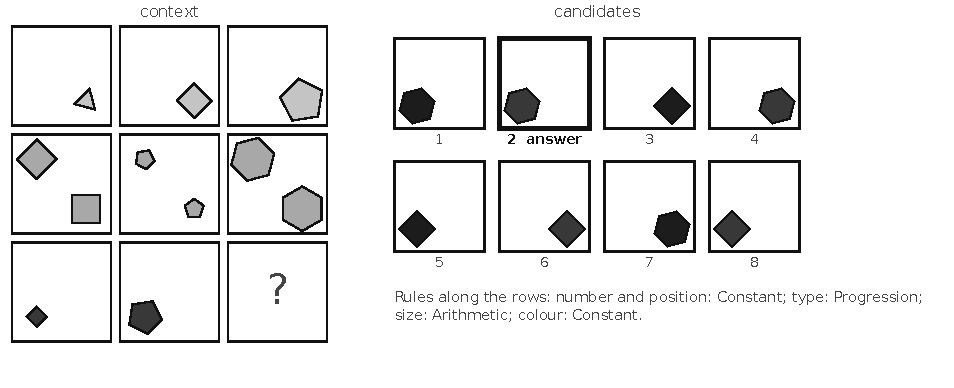
\includegraphics[width=\linewidth]{figures/iraven_puzzle}
\caption{An I-RAVEN puzzle from the distribute-four layout (training puzzle 67), drawn from its XML attributes. Along the rows, number and position follow Constant, type Progression, size Arithmetic and colour Constant. The answer is candidate 2.}\label{fig:iraven_puzzle}
\end{figure}

\begin{figure}[tbp]
\centering
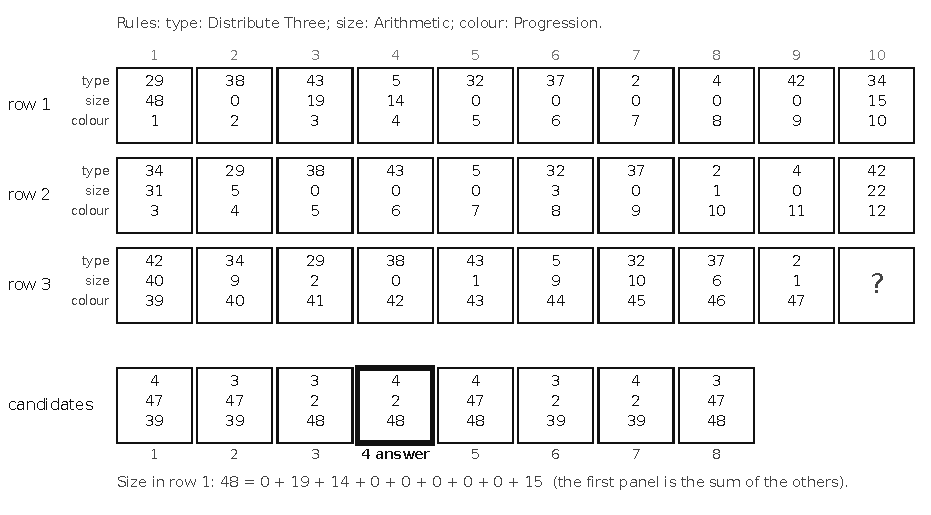
\includegraphics[width=\linewidth]{figures/iravenx_puzzle}
\caption{An I-RAVEN-X puzzle with rows of ten and values 0–50 (training puzzle 3): the last three rows of its 10 × 10 matrix, one object per panel, given as its type, size and colour values. Type follows Distribute Three, size Arithmetic and colour Progression. The answer is candidate 4.}\label{fig:iravenx_puzzle}
\end{figure}

\textbf{What generated puzzles are not.} The tests people take consist of a few dozen hand-made items, ordered from easy to hard, with no training set. The generated datasets keep the format and part of the rule list. In the RAVEN family the rules run along rows only, the list of attributes is fixed, and training and test puzzles come from one program. We measured how much depends on the row direction: after transposing an I-RAVEN matrix, 3\% of Progression instances and 1\% of Arithmetic instances still satisfy their rule, against 100\% for Distribute Three. \citet{barrett2018measuring} themselves call their generated task a different problem from the psychometric test. We therefore draw no conclusion about human reasoning from any number in this thesis, and return to what the generator contributes in Chapter~\ref{ch:8}.

\section{Graph neural networks}\label{sec:2.2}

A graph neural network keeps a vector for every node of a graph and updates it in rounds: each node collects messages from its neighbours, combines them with an operation that does not depend on their order, such as a sum or a mean, and passes the result through a learned function (\citealp{zhou2020graph}). The same functions serve every node and every edge. Two consequences matter here.

First, the network accepts graphs of any size, because its weights belong to the update rule and not to particular nodes. Second, renumbering the nodes changes nothing: the output of a node moves with the node. This permutation symmetry is the one symmetry every graph network has by construction. \citet{battaglia2018relational} describe the general point: an architecture expresses assumptions about the data, which they call relational inductive biases, and a graph network assumes that entities and their relations matter and their order does not.

What a plain graph network does not decide is everything else: which things are nodes, which edges exist, and which labels the nodes carry. A label such as ``row 1'' or ``the left component'', given to a node as an input feature, lets the network treat that row or component differently from the others. Chapter~\ref{ch:4} uses this. Two of our baselines are graph networks on the same graph, and differ only in whether nodes carry such absolute labels.

Edges join two nodes. A relation among three things, such as u + w = v among three numbers, is a hyperedge, and a network that passes messages along pairs has to be extended to use it.

\section{Lifted relational neural networks}\label{sec:2.3}

Lifted relational neural networks (\citealp{sourek2018lifted}, 2021) describe a model as a \emph{template}: a set of rules in the style of logic programming, with weights attached. A rule such as

\begin{Verbatim}[fontsize=\small,breaklines]
h(X) :- w1 : h(Y), w2 : edge(Y, X)
\end{Verbatim}

says how the value of \texttt{h} at any X is computed from the values at every Y joined to it. The variables stand for any constant. A \emph{sample} supplies the constants and the facts about them: the objects of one puzzle, their attributes, the panels they sit in.

\textbf{Grounding.} For each sample, the template and the facts are grounded: every way of substituting the sample's constants for a rule's variables that makes the rule's body derivable becomes one copy of the rule. The copies form a computation graph, with a neuron for each fact, each ground rule body, each aggregation over the bodies that share a head, and each derived atom (\citealp[Section 3.2]{sourek2021beyond}). A different sample gives a different network. The weights do not change: in the authors' words, they are shared ``in a scheme determined by the lifted structure of the template''. Variables that occur only in the body of a rule are aggregated over, which corresponds to quantifying over them. Figure~\ref{fig:grounding} shows one template grounded on two puzzles.

\begin{figure}[tbp]
\centering
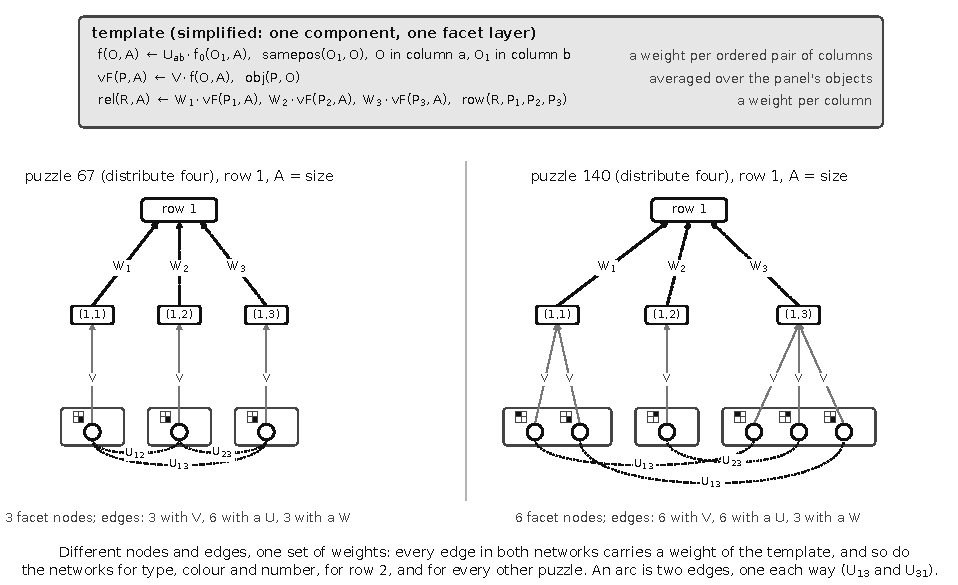
\includegraphics[width=\linewidth]{figures/grounding}
\caption{One template grounded on two puzzles (the size attribute in row 1 of each, with one facet layer). The two ground networks have different nodes and edges, but every edge carries one of the template's weights: V from a facet to its panel, W1 to W3 from the panels to the row, and U\_ab between objects at the same position in columns a and b.}\label{fig:grounding}
\end{figure}

\textbf{Relation to graph networks.} A message-passing layer is one such rule over \texttt{edge} facts, and \citet{sourek2021beyond} reproduce standard graph networks as templates. Templates go further in three ways that this thesis uses: rules over relations of any arity, so a three-way relation is as natural as an edge; rules that derive new relations from the facts before any learning takes place; and recursive rules, which unfold to whatever depth the sample's structure has. The authors list attention and gating as constructs that do not fit naturally.

\textbf{PyNeuraLogic} is the Python front end of the NeuraLogic engine. All our relational models are written in it and trained with its own optimizer, on CPU. The engine grounds each puzzle once and keeps the ground networks in memory, which sets the cost reported in Chapter~\ref{ch:5}.

The property this thesis builds on is the sentence quoted above. Chapter~\ref{ch:3} turns it into a theorem: a template cannot tell apart two constants that it does not name, so its output is unchanged by any renaming of such constants that maps the sample's facts onto themselves.

\section{Symmetry as inductive bias}\label{sec:2.4}

\textbf{Bias is necessary.} A learner that prefers no hypothesis over another cannot generalise beyond its training examples (\citealp{mitchell1980need}), and averaged over all problems no learner beats another (\citealp{wolpert1996lack}). An advantage always comes from an assumption that fits the problem. The open question is which assumptions to make, and the field disagrees on how many: \citet{sutton2019bitter} argues that general methods with more computation have overtaken hand-built knowledge again and again, while \citet{marcus2018deep} and \citet{lake2017building} argue that objects, relations and compositional structure have to be built in.

\textbf{Symmetry.} Let a group G act on the inputs of a function f. The function is \emph{invariant} if f(g·x) = f(x) for every g in G, and \emph{equivariant} if f(g·x) = g·f(x), where G also acts on the outputs. A model has a symmetry \emph{built in} when this holds for every setting of its weights, and has merely \emph{learned} it when it holds, approximately, after training. Geometric deep learning (\citealp{bronstein2021geometric}) reads the successful architectures this way: convolutional networks are equivariant to translations, group convolutions extend this to other groups (\citealp{cohen2016group}), networks on sets are invariant or equivariant to permutations (\citealp{zaheer2017deep}), as graph networks are (Section~\ref{sec:2.2}), and the architecture follows from the choice of domain and group.

\textbf{Symmetry is weight sharing.} \citet{ravanbakhsh2017equivariance} show that a layer is equivariant to a permutation group exactly when its weights are tied along the orbits of the group, and \citet{kondor2018generalization} that a layer equivariant to a compact group must be a convolution over that group. Chapter~\ref{ch:3} proves the lifted counterpart: in a template the tying is done by variables, and the group is whatever the unnamed constants and the background facts leave free.

\textbf{What a symmetry is worth.} A symmetry that the target function shares shrinks the set of functions the model can represent without removing the target, so fewer examples are needed. \citet{sokolic2017generalization} bound the generalisation error of an invariant classifier through the covering number of the base space that is left when the transformations are factored out. For T transformations that keep the transformed copies apart, this number is up to T times smaller, so the bound is up to √T smaller, which is the bound of a non-invariant classifier trained on up to T times as many examples. \citet{elesedy2021provably} prove a strict generalisation benefit for equivariant models (for squared loss and a symmetric input distribution, computed exactly for linear models), and \citet{bietti2021sample} and \citet{tahmasebi2023exact} give sample-complexity gains proportional to the size of the group for kernel methods, once the sample is large enough. These results say that the gain grows with the group. They are stated for function classes and data distributions in general; they do not say what a particular symmetry is worth on a particular rule, which is what we count in Chapter~\ref{ch:3}, and, for the components of Chapter~\ref{ch:6}, in training puzzles (Section~\ref{sec:6.2}).

\textbf{What a wrong symmetry costs.} A model can also have a symmetry that the task lacks. \citet{wang2023general} sort this into three cases, by what the symmetry does to the data. Equivariance is \emph{correct} where the transformed input also occurs in the data and has the transformed label, \emph{incorrect} where the transformed input also occurs in the data but with a different label, and \emph{extrinsic} where the transformed input lies outside the data distribution. For incorrect equivariance they prove a lower bound on the error, computed orbit by orbit: an invariant model gives every input of an orbit the same label, so on each orbit it loses at least the probability mass that does not carry the orbit's commonest label (their Theorem 4.3). The bound needs no assumption that the data's distribution is symmetric, and some invariant model attains it. Their earlier paper showed that extrinsic equivariance can help (\citealp{wang2023surprising}); this one shows that it can also hurt (their Section 5). \citet{petrache2023approximation} analyse the trade-off between the approximation error of a misspecified symmetry and its generalisation gain. The three kinds of symmetry in our Chapter~\ref{ch:3} (data symmetry, out of support, conflicting) are these three cases, reached from the generator's side, and the ceiling we compute for a conflicting symmetry is their bound evaluated on a rule's table. What we add is the other half of the count, the data a correct symmetry saves, and matched experiments in which both halves are predicted before training. Softer forms exist as well: a model can be given a preference for a symmetry and not a constraint (\citealp{finzi2021residual}; \citealp{wang2022approximately}). Chapter~\ref{ch:6} has a small result of that kind, where a model that shares all its weights but is not exactly invariant does as well as the exactly invariant one.

\textbf{Shortcuts.} A model without the right constraint may fit the training data by a rule that holds only there (\citealp{geirhos2020shortcut}). RAVEN's candidate sets are one example. Chapter~\ref{ch:6} shows another, in which a model that is allowed to tell panels apart learns one rule by the panel's address.

\textbf{Structure that matches the computation.} \citet{xu2020what} show that a network learns a task more easily when its structure mirrors the algorithm that solves it, and \citet{xu2021how} that a graph network's success in extrapolating algorithmic tasks relies on the task's non-linearities being built into the architecture or the features. Chapter~\ref{ch:7} gives a case: a model learns sums from a hundred puzzles once addition is available as a relation, and not at all without it.

\textbf{Values on a line without a zero.} A symmetry that Chapter~\ref{ch:7} turns on is the shift of all values by a constant. \citet{stevens1946theory} classifies scales by the transformations they survive: on an interval scale the zero is a convention, and only differences mean something. In geometric terms such values form an affine line, on which points can be subtracted but not added, and a weighted sum of points is defined without reference to an origin when the weights sum to one (\citealp[Lemma 2.2.1]{gallier2011geometric}). A rule c = pa + qb therefore survives a common shift exactly when p + q = 1. The midpoint of two values satisfies this and their sum does not.

\textbf{Priors and the measurement of skill.} \citet{chollet2019measure} argues that skill at a task can be bought with training data or with built-in knowledge, so a score is informative only together with both. He names the priors a fair test may assume, among them objects, elementary geometry, and small numbers with addition and subtraction (in his own benchmark, below about ten), and he counts generation from one fixed program as a weakness of a benchmark, since learning the program solves every task. RAVEN is such a benchmark. We use his terms in Chapter~\ref{ch:8} to sort our priors into those a person would bring to any such test and those read off the generator.

\section{Solvers of Raven's matrices}\label{sec:2.5}

\textbf{Black-box image models.} The first neural solvers map the images to an answer and are trained on the answer's index. WReN (\citealp{barrett2018measuring}) scores each candidate with a relation network over panel embeddings. \citet{zhuo2020solving}, the reference named in this thesis's assignment, give a ResNet the sixteen panels as one stack of images and train it on the answer's index. With ImageNet pre-training a ResNet-50 answers 86\% of RAVEN's test puzzles, above the human score that RAVEN reports, but it falls by 17 to 19 points when tested on layouts it was not trained on. Without answer labels, trained only on the assumption that the third row obeys the rules of the first two, a network reaches 28.5\%, against 12.5\% for guessing. Their results are on RAVEN, before its candidate shortcut was found. Later models add structure that matches the generator: CoPINet contrasts the candidates (\citealp{zhang2019learning}), SRAN encodes rows hierarchically (\citealp{hu2021stratified}), and SCL shares networks across objects, attributes and relations (\citealp{wu2020scattering}). Several of these are symmetry priors in our sense, and we credit them as such. All of them classify among the candidates. Reported accuracies on I-RAVEN reach about 98\%, but when \citet{malkinski2025airaven} retrained thirteen of these models under one protocol, most scored far lower: DRNet 90.9\% against a reported 97.6\%, SCL 83.4\% against 95.0\%, STSN 59.0\% against 95.7\%.

\textbf{Object-centric and graph models.} A second group first finds the objects and then reasons over them, which is the plan the assignment asks for. \citet{spratley2020closer} attend to objects before relating panels, \citet{wang2020abstract} build a multiplex graph over the objects of a puzzle, and \citet{mondal2023learning} combine slot attention with a transformer. Our facet model belongs here, with two differences: its graph has one node per attribute of an object, not per object, and it generates the answer.

\textbf{Neuro-symbolic models.} PrAE (\citealp{zhang2021abstract}) recognises the objects of each panel as probability distributions over attribute values, infers which of the generator's rules each attribute follows, executes the rule to predict the answer's attributes, and picks the nearest candidate. The rules are given. It is trained on the answer's index, through a choice among the eight candidates, with the rules of each training puzzle as an auxiliary target. This is the closest precedent for our task of generating the answer and then matching, and for the symbolic reference models of Chapter~\ref{ch:4}. ALANS (\citealp{zhang2022learning}) removes the given rules by representing values as matrices and learning operators on them. NVSA (\citealp{hersche2023neuro}) represents attributes as high-dimensional vectors and writes each rule as an expression in vector-symbolic algebra; ARLC (\citealp{camposampiero2024towards}) learns such expressions from data. In these models addition is an operation of the representation, so they compare with our models that are given addition, not with those that have to learn sums (Chapter~\ref{ch:7}).

\textbf{Language models.} Given the attribute values as text, large language models solve many of these puzzles without training on them. \citet{hersche2024towards} report that GPT-4, given the attribute values as text, answers 93\% of I-RAVEN's centre puzzles and 77–82\% of I-RAVEN-X puzzles with rows of 10, and that on Arithmetic at range 50 it reaches 30\% where the learned ARLC reaches 82\%.

\textbf{Arithmetic in neural networks.} Networks that are not given addition learn it poorly. \citet{trask2018neural} find that networks trained on sums fail outside the trained range and describe the failure as memorisation. Small transformers trained on modular addition first memorise and, much later, generalise (\citealp{power2022grokking}), by representing each number as an angle so that adding becomes rotating (\citealp{nanda2023progress}). \citet{mohamadi2024why} prove that a permutation-equivariant kernel method, which is how a network behaves early in training, must see a constant fraction of the table of modular addition before it generalises. That is the situation of a model with separate weights for every value, and in Chapter~\ref{ch:7} such a model tracks a learner that only memorises.

\section{Where this thesis stands}\label{sec:2.6}

Three things separate this work from the solvers above.

\begin{itemize}
\item \textbf{The question is the price of a prior, not the score.} The models above each add structure and report accuracy. We take one model family and add or remove one symmetry at a time, at several amounts of training data, and compare each result with a number computed before training.
\item \textbf{The symmetry is declared.} In a template a symmetry is the absence of a name, and one theorem covers every symmetry built this way. The architectures above are each engineered for their symmetry, and each needs its own argument.
\item \textbf{The answer is generated and the candidates are never seen}, in training or as input. Only PrAE and its successors also generate the answer before matching, and they are given the rules or the operations; PrAE is still trained through a choice among the candidates.
\end{itemize}

\chapter{Symmetry in a lifted template}\label{ch:3}

This chapter holds the theory of the thesis. Its first half explains how a symmetry gets into a lifted template and why it then holds exactly. A template cannot tell apart constants that it does not name (Sections~\ref{sec:3.1} and \ref{sec:3.2}). What the template names and which background facts it is given decide, together, which group the model has (Section~\ref{sec:3.3}). The same theorem shows two different ways of taking a symmetry out again (Section~\ref{sec:3.4}). Section~\ref{sec:3.5} sorts symmetries by what they do to the puzzles a generator produces. The second half puts a price on a symmetry before any training: the data it saves and the ceiling it sets (Sections~\ref{sec:3.6} and \ref{sec:3.7}).

None of the proofs is long. What the chapter adds is that every statement is tied either to a check that needs no training or to a count that was made before the runs of Chapters~\ref{ch:6} and \ref{ch:7}.

\section{Templates, samples and renamings}\label{sec:3.1}

We use the setting of Section~\ref{sec:2.3}. A template T is a set of weighted rules. Most arguments of its atoms are variables, but a rule may also write a constant. The rule body \texttt{col(P, "c1")}, for example, holds only for panels of the first column. We call the constants written in T its \emph{named} constants.

A sample is a set of facts F. Here a sample is one puzzle, or one component of one puzzle (Section~\ref{sec:4.4}), and its facts are of two sorts. The \emph{puzzle facts} describe what the panels show: which objects a panel holds, which component an object belongs to, and the value of each attribute. The \emph{background facts} describe the frame the puzzle sits in, which is the same for every puzzle of a dataset: which panels form a row, which rows are complete, which column a panel stands in, and, for the value-axis model of Section~\ref{sec:4.5}, how the values relate to each other. Grounding T on F gives a network in which every atom a has a value. We write it \(\mathrm{val}_F(a)\).

A \emph{renaming} σ is a one-to-one map from constants to constants. It acts on a fact or an atom by renaming every constant in it, and on a set of facts one fact at a time. A transformation g of a puzzle \emph{is a renaming} if some σ turns the facts of the puzzle into exactly the facts of the transformed puzzle. Exchanging rows 1 and 2 is a renaming: it swaps the panels of the two rows and the row names r1 and r2. Mirroring a left-right puzzle renames the components k0 and k1 into each other. Exchanging size and colour renames the two attributes. Not every transformation is a renaming. Moving an object to another slot of a grid changes a vector of numbers inside a fact, not a constant, and no σ does that.

As in Section~\ref{sec:2.4}, a model has a symmetry \emph{built in} if f(g·x) = g·f(x) for every setting of its weights. For a renaming this has a plain meaning: the output on the transformed puzzle is the output on the original, with its atoms renamed. If no output atom contains a renamed constant, as when rows are exchanged, the symmetry is an invariance. If some do, as the output blocks for size and colour do, it is an equivariance.

\section{The renaming theorem}\label{sec:3.2}

\textbf{Theorem.} Let σ be a renaming that leaves every named constant of T in place. Then for every atom a and for every setting of the weights,

\[ \mathrm{val}_{\sigma(F)}(\sigma(a)) = \mathrm{val}_F(a). \]

\emph{Proof.} A ground rule is a rule r of T whose variables have been replaced by constants through a substitution θ. Since σ leaves the constants of r in place, renaming the ground rule rθ gives r(σ∘θ). That is a ground rule of the same rule r, and its body holds in σ(F) exactly when the body of rθ holds in F. The inverse of σ also leaves the named constants in place, so this pairs the ground rules of the two networks one to one. Weights belong to the rules of T and not to their groundings, so paired ground rules carry the same weights. An aggregation, such as an average or a sum, sees the multiset of values of the bodies that share a head, and σ maps this multiset one to one onto its counterpart. A product or a concatenation combines the atoms of a single body, and σ maps those one by one. For the facts, the equation holds by the definition of σ(F). The ground network has no cycles, so induction over the depth of an atom carries the equation from the facts to every atom. ∎

A transformation of the puzzle is therefore built in whenever two conditions hold:

\begin{enumerate}
\item it is a renaming: some σ turns the facts of the puzzle, background facts included, into exactly the facts of the transformed puzzle;
\item the template names none of the constants that σ moves.
\end{enumerate}

Three remarks.

\begin{itemize}
\item The conditions are sufficient, not necessary. A template can also be symmetric by coincidence, for instance when two rules that name different constants happen to have equal weights.
\item A named constant allows the symmetry to break, but does not force it. The checks below show that with random weights it does break.
\item The theorem is the form that the permutation equivariance of graph networks takes in a logic program. In a graph network the renamed constants are the nodes, and the only facts are edges and node features, which a permutation of the nodes maps onto themselves. In a template any constant can take that role: a row, a component, an attribute, a value. The background facts decide which renamings keep the frame of the puzzle.
\end{itemize}

\textbf{The checks.} Every built-in symmetry claimed in this thesis was also checked numerically, without training. With random weights, several draws and unseen puzzles, the output on the transformed puzzle is compared with the renamed output on the original (\texttt{core/pynl/facet\_symmetry\_check.py}, and the \texttt{--check-shift} and \texttt{--check-scale} options of \texttt{core/pynl/value\_axis.py}). Where the theorem applies, the largest difference lies between 0 and 10⁻¹⁵, the size of a change in the order of a floating-point sum. Where the template names a constant that the transformation moves, the output changes by 0.4 to 1.0. Sections~\ref{sec:3.3} and \ref{sec:3.4} give the individual numbers.

\section{What is named, and what the background facts keep}\label{sec:3.3}

The two conditions of the theorem are two places to put a symmetry. The rules decide which constants are named, and the background facts decide which renamings map a sample onto itself. Together they fix the group of the model: the renamings that leave every named constant in place and keep every background fact true. Adding a background relation can only make this group smaller, because each new fact is one more thing a renaming must keep. The background facts are therefore where a lifted template chooses its group, in the way that the choice of domain fixes the group of a convolutional or a graph network (Section~\ref{sec:2.4}).

The relations used in this thesis show how this works.

\begin{itemize}
\item \textbf{Complete rows}, \texttt{full(r1)} and \texttt{full(r2)}. Both complete rows carry the same fact, and the rules reach them only through it, so exchanging rows 1 and 2 keeps the frame. The question row is set apart, because the rules name it, as in \texttt{inrow(P, "r3")}, and no renaming may move it.
\item \textbf{Columns}, \texttt{col(P, "c1")}, \texttt{col(P, "c2")} and \texttt{col(P, "c3")}. The rules name each column, so no exchange of columns is built in. That is intended: a Progression row read backwards is a different row. For I-RAVEN-X with rows of ten, \emph{column roles} give each panel one of the facts \texttt{col(P, "first")}, \texttt{col(P, "mid")} and \texttt{col(P, "last")} instead. All eight middle columns now carry the same fact, so any exchange of middle columns is built in, while the first and last columns stay apart.
\item \textbf{Neighbours}, \texttt{next(P, Q)}. The row fold of Appendix~\ref{app:E} reads a row as a chain of neighbouring panels. Reversing a row would map \texttt{next} onto its inverse, which is not among the facts, so the fold keeps the direction of a row.
\item \textbf{Offsets on the value axis}, \texttt{off(U, V, k)} for V = U + k. In the value-axis model every value is a constant, and no rule names one. Moving all values by the same amount s maps \texttt{off} onto itself, exactly on a ring of values and away from the ends on a line, so the model is equivariant to this common shift.
\item \textbf{Addition}, \texttt{plus(U, W, V)} for U + W = V. The common shift does not keep these facts, since (u + s) + (w + s) is not (u + w) + s. Giving a model \texttt{plus} therefore takes the common shift out of its group. What remains are the moves that addition keeps, such as adding s to one operand and to the result.
\end{itemize}

\begin{center}\small
\begin{tabularx}{\linewidth}{@{}YYYY@{}}
\toprule
background facts & the renaming they keep & built in & random weights, largest change \\
\midrule
\texttt{full(Rw)} & rows 1 and 2 exchanged & yes & 3·10⁻¹⁶ \\
\texttt{col(P, c)}, one fact per column & no exchange of columns & no & columns 1 and 2: 0.46 to 0.96 \\
\texttt{col(P, "mid")}, column roles & any two middle columns exchanged & yes & 4.4·10⁻¹⁶ (named columns: 0.38) \\
\texttt{off(U, V, k)} & all values moved by the same amount & yes & 3·10⁻¹⁷ \\
\texttt{off} and \texttt{plus} & one operand and the result moved together & the common shift no longer & 0 in 94–97\% of puzzles; up to 2.8·10⁻³ where the shift changes a sum \\
\bottomrule
\end{tabularx}
\end{center}

The same mechanism lets a symmetry be stated as a relation, not only left unnamed. The two components of the left-right and up-down layouts are exchangeable because no rule names k0 or k1. One could also give the model a relation that says how the components of a layout correspond, for example a reflection with one fact per layout, and let every rule take the layout as a variable. The left-right and up-down layouts would then share every weight because no rule names either of them, and the relation would tell the model which component of one layout corresponds to which of the other. The experiments did not need this. It is the form in which the method reaches from the symmetries inside one puzzle to symmetries between layouts.

\section{Two ways to break a symmetry}\label{sec:3.4}

To measure what a symmetry is worth, Chapter~\ref{ch:6} takes it out of a model and compares. The theorem has two conditions, and there is one way to break each.

\textbf{Labels} break the first condition. The template stays as it is, but facts tie each of the exchangeable constants to a fixed vector: \texttt{cid(k0) = [1, 0]} and \texttt{cid(k1) = [0, 1]} for the components, or a one-hot \texttt{aid(A)} for the attributes, read by the summary of every panel. When a puzzle is mirrored, its objects move from k0 to k1, but \texttt{cid(k0)} stays [1, 0]. The facts of the mirrored puzzle are then no longer a renaming of the original facts. With random weights the mirror changes the output by 0.37, and with attribute labels the exchange of type and colour changes it by 0.41. Every weight is still shared between the components or the attributes. The labels add 320 weights to the 266,528 of the components model, or 512 to the 288,328 of the attributes model.

\textbf{Separate weights} break the second condition. Every rule with weights is written once per component, or once per attribute, with that constant in it. The template now names the constants, and the pairing of ground rules in the proof is gone: the rules for k0 and those for k1 have weights of their own. With random weights the mirror changes the output by 0.78, and the exchange of type and colour by 0.90. At the same widths the model has twice as many weights for the components and 3.2 times as many for the attributes, so Chapter~\ref{ch:6} also uses narrower versions with as many weights as the symmetric model.

The two ways take out different things. Labels remove the exact invariance and keep the sharing: every training puzzle still trains every weight. Separate weights remove both. Comparing a symmetric model with its labelled and its separate versions therefore tells apart what the invariance is worth and what the sharing is worth (Section~\ref{sec:6.3}).

A constant can also be named by accident. The first version of the copy links in Section~\ref{sec:6.5} gave every panel a gate of its own, \texttt{gate("p3")}. That names the panels, so the exchange of rows 1 and 2 was no longer built in (0.99 with random weights), and the trained model made use of the freedom. Gates computed from what a panel contains name nothing, and with them the exchange is exact again (4.4·10⁻¹⁶).

\section{Three kinds of symmetry}\label{sec:3.5}

Whether a built-in symmetry helps or hurts depends on what it does to the puzzles that the generator produces. Take a transformation g of a complete matrix that leaves the missing panel in its place, a valid puzzle x and its answer y. There are three cases.

\begin{itemize}
\item \textbf{A data symmetry.} g·x is again a valid puzzle, its answer is g·y, and the generator produces g·x as often as x. The training data then contains both, and a model with the symmetry has less to learn. This is a case of what \citet{wang2023general} call correct equivariance; their definition asks only that g·x occur in the data, not that it occur as often. Section~\ref{sec:3.6} counts what it is worth.
\item \textbf{Out of support.} The generator never produces g·x, so the symmetry puts no constraint on the data. This is Wang et al.'s extrinsic equivariance. For the benchmark two cases of it differ. If g·x is still a valid puzzle with the answer g·y, the symmetry belongs to the task but not to the data. Building it in costs nothing on the right solution, and it rules out solutions that hold only on what the generator produces (Section~\ref{sec:6.5}). If g·x is not a valid puzzle at all, the model never has to answer it, so no ceiling follows, but the model must find the rule in a form that respects g, and that can cost data (Section~\ref{sec:6.7}).
\item \textbf{Conflicting.} g·x is a valid puzzle that the generator does produce, but its answer is not g·y. A model with the symmetry has to answer x and g·x consistently, so it is wrong on one of them. This is Wang et al.'s incorrect equivariance, for which they prove a lower bound on the error, orbit by orbit. Section~\ref{sec:3.6} evaluates that bound on a rule's table, and Sections~\ref{sec:6.7} and \ref{sec:7.4} test it.
\end{itemize}

Wang et al. make their definitions point by point, so one move can be correct on some rules and incorrect on others, as the shift is.

Which case a transformation falls into is a property of the generator. It can be read off the generators' code and checked on the data. The table gives the share of rule instances (one attribute of one puzzle) that still satisfy a rule of the same kind after the transformation, in the order Constant / Progression / Arithmetic / Distribute. Before the transformation every instance satisfies its own rule.

\begin{center}\small
\begin{tabularx}{\linewidth}{@{}YYYY@{}}
\toprule
transformation & I-RAVEN & I-RAVEN-X, rows of 3 & I-RAVEN-X, rows of 10 \\
\midrule
rows 1 and 2 exchanged & 100 / 100 / 100 / 100 & 100 / 100 / 100 / 100 & 100 / 100 / 100 / \textbf{0} \\
columns 1 and 2 exchanged & 100 / \textbf{0} / 51 / 100 & 100 / \textbf{0} / 55 / 100 & 100 / \textbf{0} / 50 / \textbf{0} \\
two middle columns exchanged & – & – & 100 / \textbf{0} / 100 / \textbf{0} \\
values reflected, v → max − v & 100 / 100 / \textbf{0} / 100 & 100 / 100 / \textbf{0} / 100 & 100 / 100 / \textbf{0} / 100 \\
matrix transposed & 58 / 3 / 1 / 100 & – & – \\
\bottomrule
\end{tabularx}
\end{center}

The symmetries that this thesis builds in, breaks or adds on purpose fall into the three cases as follows.

\begin{center}\small
\begin{tabularx}{\linewidth}{@{}YYYY@{}}
\toprule
symmetry & case & the reason, from the generator & used in \\
\midrule
order of the objects in a panel; order of the candidates & data & the order carries no meaning & every model \\
the two components of the left-right and up-down layouts & data & identical constraints, and matching rule counts and means in both components & 6.2, 6.3 \\
size and colour exchanged (I-RAVEN-X) & data & both are drawn by the same function, with the same rules and range & 6.2, 6.3 \\
the attributes exchanged, apart from size and colour in I-RAVEN-X & out of support & the attributes differ in their values (in I-RAVEN they have 5, 6 and 10) and type never carries Arithmetic & 6.4 \\
rows 1 and 2 exchanged, I-RAVEN and rows of 3 & data & each row is drawn afresh by the same rules, with one small exception for Arithmetic on colour & 6.2 (the vision transformer), 6.5 \\
rows 1 and 2 exchanged, rows of 10 & out of support, valid & a Distribute row is the first row rotated by a step, and after the exchange no step fits; the answer is still the value that the third row lacks & 6.5 \\
middle columns exchanged, rows of 10 (column roles) & out of support: valid for Arithmetic and for the answer of Distribute, not for Progression & the operands of a sum may be reordered and the value a row lacks does not depend on the order, but the generator places the zeros among the operands in a fixed pattern & 6.6 \\
columns 1 and 2 tied & out of support, not valid & a Progression row read in another order is not a Progression row & 6.7 \\
values reflected (a model that cannot tell v from max − v) & conflicting & Constant, Progression and Distribute rows stay valid and equally likely with the reflected answer, which differs & 6.7 \\
all values moved by the same amount & data for Constant, Progression, Distribute and midpoint, exactly on a ring of values; conflicting for sum and Arithmetic & a shifted sum row is not a sum row, but its question row is a valid question with another answer & 6.2, 7.3–7.6 \\
\bottomrule
\end{tabularx}
\end{center}

\section{Pricing by orbits}\label{sec:3.6}

A symmetry merges inputs into orbits. This section counts what that is worth on a rule's table, in the simplest setting where the count can be made exactly: a single row of three values. First the words.

A \textbf{row} is three values (a, b, c). In the \textbf{question row} the third is missing, and a \textbf{learner} is anything that turns the two values (a, b) into an answer for c. We write f(a, b) for that answer.

A \textbf{move} changes a row in a fixed way. Three moves matter here:

\begin{itemize}
\item the \textbf{shift}: add the same number s to all three values;
\item \textbf{scaling}: multiply all three values by the same number k;
\item \textbf{one operand with the answer}: add s to a and to c, or to b and to c.
\end{itemize}

A rule \textbf{keeps} a move if every row of the rule is again a row of the rule after the move. A learner \textbf{has} a move if moving its input moves its answer in the same way: for the shift, f(a + s, b + s) = f(a, b) + s. The \textbf{orbit} of an input is everything the moves turn it into. Values are the whole numbers 0 to 50. Where a statement divides, it is made on the ring of 101 values that the models use, where every step has a half and every multiple.

\subsection{Which rule keeps which move}\label{sec:3.6.1}

\textbf{Statement 1.} A rule of the form c = pa + qb keeps the shift exactly when p + q = 1. Every such rule keeps scaling. Sum keeps the move of one operand with the answer, and midpoint does not.

\emph{Why.} Shift a row of the rule by s. The new third value is c + s. The rule asks for p(a + s) + q(b + s), which is pa + qb + (p + q)s, that is c + (p + q)s. The two agree for every s exactly when p + q = 1. Midpoint has ½ + ½, mirror (c = 2a − b) has 2 − 1, Progression (c = 2b − a) has −1 + 2 and Constant (c = b) has 0 + 1: all keep the shift. Sum has 1 + 1 = 2 and does not. For scaling, multiply the rule by k: kc = p(ka) + q(kb), which holds whatever p and q are. For the last move, add s to a and to c in a sum row: c + s = (a + s) + b holds; in a midpoint row the rule asks for c + s/2.

\emph{Checked on the tables} (rows that are rows again after the move, of those that stay in range):

\begin{center}\small
\begin{tabularx}{\linewidth}{@{}YllY@{}}
\toprule
 & shift & scaling by 2, 3, 5 & one operand with the answer \\
\midrule
sum, 1,225 rows & 0 of 30,325 & 465 of 465 & 39,200 of 40,425 \\
midpoint, 1,250 rows & 40,400 of 40,400 & 490 of 490 & 0 of 51,450 \\
mirror, 1,250 rows & 40,400 of 40,400 & 490 of 490 & 0 of 51,450 \\
\bottomrule
\end{tabularx}
\end{center}

The 3\% that sum loses under its own move are rows pushed onto a = 0, which the table leaves out.

\subsection{A learner with the shift, and what it saves}\label{sec:3.6.2}

\textbf{Statement 2.} A learner that has the shift can only compute c = b + g(b − a), for some list of numbers g with one entry per first step b − a.

\emph{Why.} Shift the input by −a. The learner must answer (0, b − a) with f(a, b) − a. So f(a, b) = a + f(0, b − a): its answer is a plus something that depends on the first step alone. Writing g(d) for f(0, d) − d gives f(a, b) = b + g(b − a). All inputs with the same first step form one orbit, and the learner has one free number for each orbit.

\textbf{Statement 3 (the data saved).} If the rule keeps the shift, one training row teaches the learner every row with the same first step. With rows drawn evenly from a table in which orbit o holds a share P(o) of the rows, the expected share of unseen rows whose orbit n training rows have reached is

the sum over orbits of P(o) · (1 − (1 − P(o))ⁿ).

\emph{Why.} A rule that keeps the shift is itself of the form c = b + g*(b − a), by the argument of Statement 2 applied to the rule. A training row with first step d shows g*(d), and that is the right entry for every row with that first step. An unseen row is therefore answered correctly exactly when its first step occurred in training. A given orbit is missed by one training row with chance 1 − P(o) and by n independent rows with chance (1 − P(o))ⁿ. An unseen row lies in orbit o with chance P(o). Adding up over the orbits gives the formula. The same holds for any set of moves the rule keeps, with its own orbits.

\emph{Checked on midpoint.} ``Expected'' uses the table alone. ``Reached'' is the counting learner on the actual training puzzles, which keeps one answer per orbit and is told the rule. 100 and 600 training puzzles hold 57 and 311 midpoint question rows.

\begin{center}\small
\begin{tabularx}{\linewidth}{@{}YlYYl@{}}
\toprule
built in & orbits & 100 puzzles: expected / reached / trained network & 600 puzzles & rows for 90\% \\
\midrule
nothing, one answer per pair (a, b) & 1,250 & 4.5 / 5.0 / 5.0 ± 0.5 & 22.0 / 21.6 / 18.0 ± 0.9 & 2,878 \\
the shift & 50 & 74.8 / 80.0 / 59.9 ± 4.5 & 98.7 / 99.8 / 98.3 ± 1.9 & 107 \\
the shift and doubling & 26 & 90.5 / 94.3 / 89.2 ± 2.7 & 99.3 / 99.8 / 99.2 ± 0.2 & 55 \\
the shift and scaling & 1 & 100 / 100 / 100.0 & 100 / 100 / 100.0 & 1 \\
\bottomrule
\end{tabularx}
\end{center}

The formula gives the counting learner's score to within 6 points before a single puzzle is drawn. The shift cuts the rows needed for 90\% from 2,878 to 107, a factor of 27. The trained networks are within 4 points of the counted value without a symmetry. With one they are under it where many orbits are left and little data is given: by 20 points with the shift and by 5 with doubling at 100 puzzles, by 2 or less at 600, and by nothing with scaling. The three networks with a symmetry are those whose row descriptor reads the steps (Section~\ref{sec:7.7}); Section~\ref{sec:3.7} says why that matters.

\subsection{The ceiling, and whose ceiling it is}\label{sec:3.6.3}

\textbf{Statement 4 (the ceiling).} On a rule in which the rows of an orbit all need different answers, a learner of the form of Statement 2 is right on at most one row of each orbit. For sum under the shift that is 97 rows of 1,225: 7.9\%.

\emph{Why.} On a sum row the answer is b + a, so the learner is right exactly when g(b − a) = a. Rows with the same first step have different a, and g holds one number for that step. It can match one of them. Sum's table has 97 different first steps. With rows drawn evenly, the best a learner can expect is one right row per orbit, 97 in 1,225. In general the count per orbit is the largest group of its rows whose answers agree once the move is undone; for the shift, the rows with the same c − b. Written this way a learner with the shift is a learner of c − b that ignores the shift, and the count is the bound of \citet[Theorem 4.3]{wang2023general} for such learners, evaluated here on a table.

\emph{Checked.} Fitted on the whole table, the counting learner with the shift is right on 97 of 1,225 rows. With the shift and doubling it is 88 (7.2\%), with the shift and scaling 17 (1.4\%). The trained shared model reaches 4.5 ± 2.3 and 6.2 ± 0.8 at 100 and 600 puzzles and 7.1 at 6,000, at the epoch picked on the selection puzzles.

\emph{How sharp the check is.} The ceiling is on the expected accuracy. The unseen set has 507 sum rows, on which one standard deviation of a 7.9\% rate is 1.2 points. Over all 172 evaluated epochs of the nine runs, 8 are above 7.9 and the highest is 9.7, in the run on 6,000 puzzles, whose epochs average 7.9. So the model sits at the ceiling, within what chance allows on this many rows, and the measurement cannot exclude a point or two above it. Statement 5 says why a point or two would not contradict anything.

\textbf{Statement 5 (the ceiling belongs to learners that answer from the question row).} A model that has the shift of the whole puzzle, all nine panels together, is not capped on sum by that symmetry alone.

\emph{Why.} Here is a function of the whole puzzle that uses only differences:

c₃ = b₃ + (c₁ − b₁) + (a₃ − a₁).

Shift every panel by s and the answer moves by s, so the function has the shift. On a sum puzzle c₁ − b₁ is a₁, so the function returns b₃ + a₁ + a₃ − a₁ = a₃ + b₃, the right answer. A complete sum row shows where zero is, and a learner that can measure from a panel of one row to a panel of another can use it.

\emph{Checked.} The function is right on 507 of 507 unseen sum rows and follows a shift of the whole puzzle on all of them.

\emph{What this means for the trained model.} Statements 2 to 4 are proved for a learner that sees the question row. The template sees the whole puzzle. It stays under the ceiling because of how it reads the puzzle, which can be read off its rules: the score of a candidate value V is computed from V's offsets to the two panels of the question row, from how many panels of each row sit exactly at V, and from a descriptor of the puzzle that is the same for every V. No rule measures the offset between a panel of the question row and a panel of another row. So apart from values that happen to coincide between rows, the template is a learner of the form of Statement 2, with a g that may depend on the descriptor. The rows of an attribute are drawn independently, so the descriptor of the complete rows says nothing about where the question row sits. For the template the ceiling is therefore a prediction that follows from its structure, and not a consequence of the puzzle-wide shift alone. The coincidences are a real way past it, though a small one: in 48 of the 507 unseen sum rows the answer is a value that already stands in the puzzle, and the template sees which values those are. The runs sit at the ceiling and not clearly above it.

In the terms of \citet{wang2023general}: shifting one row turns a sum row into a row that needs another answer, which is their incorrect equivariance, the case their lower bound covers. Shifting a whole sum puzzle turns it into something that is not a sum puzzle at all, which is their extrinsic equivariance. On such orbits only one puzzle occurs in the data and their bound is zero. Extrinsic equivariance can still hurt (\citealp[Section 5]{wang2023general}) or help (\citealp{wang2023surprising}).

\subsection{More of the rule's moves}\label{sec:3.6.4}

\textbf{Statement 6 (doubling).} A learner that has the shift and doubling has one free number for each odd part of the first step. On the ring, a row with a first step it never saw is answerable exactly when a training row had a first step with the same odd part.

\emph{Why.} By Statement 2 the learner computes b + g(d). Doubling the input must double the answer's offset from b, so g(2d) = 2g(d). Write a step as d = m·2ʲ with m odd. Then g(d) = 2ʲ·g(m): the entry for the odd part fixes the entries for all its doublings, and one training row with any of them fixes g(m). Midpoint's even first steps between −50 and 50 have 26 odd parts.

\emph{Checked.} At 100 puzzles 101 unseen midpoint rows have a new first step: 72 with an odd part that training had, 29 without. The trained doubled model is right on 50 / 43 / 39 of the 72 and on 0 / 0 / 0 of the 29, over three seeds. The model with the shift alone is right on none of the 101.

\textbf{Statement 7 (scaling).} On the ring, a learner that has the shift and every scaling computes c = a + t·(b − a) for one number t, on every row with a ≠ b.

\emph{Why.} Any two different values (a, b) are the image of (0, 1) under ``multiply by b − a, then add a''. The learner has both moves, so f(a, b) = (b − a)·f(0, 1) + a. Its only free number is t = f(0, 1). Midpoint is t = ½, Progression is t = 2, mirror is t = −1.

\emph{A consequence that is also proved.} With scaling built in, every question row with two different values is the same input, (0, 1). The question row then says nothing about which rule applies. Midpoint and Progression need different t, so a model with scaling can tell them apart only from the complete rows.

\emph{Checked.} The counting learner with these moves is right on every midpoint row after the first training row. On sum its ceiling is 17 rows of 1,225. The consequence is what Section~\ref{sec:7.7} measured, in both directions. With a row descriptor that came out the same for every row, the scaled model continued four midpoint rows in five as a Progression at two seeds of three. With a descriptor that reads each pair's step, it is right on all 505 midpoint rows in six runs of six, from 100 puzzles and from 600, and the descriptor separates the two rules in every run.

\textbf{Statement 8 (addition's own moves).} A learner that has both moves of one operand with the answer computes c = a + b + k for one number k.

\emph{Why.} Move the first operand by −a and the second by −b: the learner must answer (0, 0) with f(a, b) − a − b. So f(a, b) = a + b + f(0, 0).

\emph{Checked.} The counting learner with these moves is right on every sum row after one training row. The shared model given the \texttt{plus} facts reaches 98.2 ± 0.8 on sum from 100 puzzles and 99.7 ± 0.4 from 600.

\textbf{Statement 9 (one orbit is the rule, up to one answer).} If the moves a learner has can turn any input into any other, the learner is fixed by its answer to one input.

\emph{Why.} Pick an input x. Every other input is some move h applied to x, and the learner must answer it with h applied to its answer to x. Nothing else is free.

This is why the number of orbits is the right unit: it counts the answers that are left to learn. Statements 7 and 8 are the two cases with one orbit, and in both the model has been handed its rule up to one number.

\subsection{Values read as numbers}\label{sec:3.6.5}

\textbf{Statement 10.} Let the rule be c = pa + qb, and let the two complete rows of a puzzle be (a₁, b₁, c₁) and (a₂, b₂, c₂). If a₁b₂ ≠ a₂b₁, the two rows fix p and q, a least-squares fit finds them, and its answer for the question row is exact. Nothing is learned from other puzzles.

\emph{Why.} The two rows are two equations, a₁p + b₁q = c₁ and a₂p + b₂q = c₂. They have exactly one solution when a₁b₂ ≠ a₂b₁, and the rule's own p and q are a solution. Least squares returns the exact solution when there is one. When a₁b₂ = a₂b₁ the rows leave a whole line of solutions, and the fit returns the shortest, which need not be the rule's.

\emph{Checked} (\texttt{analysis/twins\_linear\_fit.py}, unseen puzzles, no training):

\begin{center}\small
\begin{tabular}{@{}lllll@{}}
\toprule
puzzles & the fourth rule & Progression & Constant & Distribute Three \\
\midrule
sum & 99.6 & 98.7 & 100 & 0 \\
midpoint & 99.8 & 99.3 & 100 & 0 \\
mirror & 99.8 & 98.7 & 100 & 0 \\
lookup & 1.7 & 98.6 & 100 & 0 \\
\bottomrule
\end{tabular}
\end{center}

All 44 misses on the linear rules (13, 7, 12 and 12) are puzzles with a₁b₂ = a₂b₁. There is no miss among the others. Lookup and Distribute Three are not of the form, and the fit gets 1.7\% and nothing.

\subsection{Reach: what is proved and what is measured}\label{sec:3.6.6}

\textbf{Statement 11.} For a learner with one free number per orbit, training rows from other orbits put no condition on the number of an orbit that training never reached.

\emph{Why.} By Statement 2 the learner's answer on a row depends on g at that row's first step only. A training row with another first step involves another entry of g. So every setting of the unreached entry fits the training rows equally well, and the training data cannot make it right.

\emph{Proved for:} the counting learner. \emph{Measured for the networks:} the kernel has one free weight vector per offset, and nothing ties the vectors of different offsets together. The template therefore has no way to carry ``half the step back'' from the steps it has seen to one it has not, beyond coincidences of weights trained in other roles; Statement 11 applies to it nearly as it stands. The measurement is a check of that, not a discovery about networks. What the count adds is that it says before training which rows those are. Pooled over three seeds:

\begin{center}\small
\begin{tabularx}{\linewidth}{@{}Ylll@{}}
\toprule
training rows in the row's orbit & 0 & 1 & 3–4 \\
\midrule
shared model, 100 puzzles & 0 of 303 & 422 of 573 (74\%) & 172 of 186 (92\%) \\
shared model, 600 puzzles & 0 of 3 & 71 of 72 (99\%) & 89 of 90 (99\%) \\
weights per value, 100 puzzles (orbit: the pair) & 11 of 1,440 (1\%) & 65 of 75 (87\%) & – \\
\bottomrule
\end{tabularx}
\end{center}

With no training row in its orbit a row is never right, beyond the 1\% that guessing among 101 values gives. With one it usually is. So which unseen rows a model of this family answers can be listed from the training set before training: the rows whose orbit it reached.

\section{The ladder}\label{sec:3.7}

Statements 2, 6, 7 and 10 put the models in one order, by how much of the rule's group is built in and how many answers are left to learn. Midpoint at 100 training puzzles:

\begin{center}\small
\begin{tabularx}{\linewidth}{@{}YYYlY@{}}
\toprule
built in & left to learn & expected from the table & counting learner & trained model \\
\midrule
nothing about the values & 1,250 rows & 4.5 & 5.0 & 5.0 ± 0.5 \\
the shift & 50 orbits & 74.8 & 80.0 & 59.9 ± 4.5 \\
the shift and doubling & 26 orbits & 90.5 & 94.3 & 89.2 ± 2.7 \\
the shift and scaling & 1 orbit, one number & 100 & 100 & 100.0 / 100.0 / 100.0 \\
the linear form, values as numbers & nothing from other puzzles & – & – & 99.8, no training \\
\bottomrule
\end{tabularx}
\end{center}

For sum the ladder has other rungs, because its moves are others: nothing (4.8 ± 0.6); the shift, with the answer read from the question row, which sum does not keep (4.5 ± 2.3 at a ceiling of 7.9); its own moves (98.2 ± 0.8); the linear form (99.6, no training).

The count says each rung needs less data than the one below, and the trained models end in the same order. They do so only at the second attempt, and they do not reach the count's numbers on every rung. With the first row descriptor the two scaling rungs fell below the rung beneath them: 49.9 ± 5.3 with doubling and 19.0 / 100.0 / 21.0 with scaling. Statement 7's consequence names the reason: with rows read in a unit the rule has to come from the complete rows, and that descriptor did not carry it. A descriptor that reads each pair's step was then built, with its outcome predicted before the runs, and gives the table above (Section~\ref{sec:7.7}). The first attempt is a result in its own right: the same group and the same orbit count gave 20\% or 100\% depending on how a row was described. The count is a bound for a learner that shares nothing across orbits and can tell every orbit apart. It predicts the order of the rungs and which rows a model can get, not the accuracy a particular network reaches; with the shift alone the network stays 20 points under the counting learner at 100 puzzles (59.9 against 80.0), and we did not find the cause.

\subsection{What is not proved}\label{sec:3.7.1}

\begin{itemize}
\item \textbf{That the trained network reaches the count.} The count is what a learner with one answer per orbit gets. The networks come within 4 points of it without a symmetry, and with the shift they stay 20 points under it at 100 puzzles and 2 at 600. A network reaches the count only if it can tell the orbits apart, which a row descriptor that pools away the steps prevents (Section~\ref{sec:7.7}). The 20 points with the shift alone may be a limit of the same kind; it is not explained here.
\item \textbf{That a network cannot generalise past its orbits.} Statement 11 is proved for the counting learner. For the networks it is a measurement on one family of templates, in which nothing but the built-in moves ties weights together. A model with other ties, such as a smooth kernel, could do otherwise.
\item \textbf{The ceiling for the template.} Statement 5: it follows from how the template reads the puzzle, with coincidences of values between rows left over. It is not a theorem about the puzzle-wide shift. The runs sit at it: 7.1 or less at every picked epoch, and above 7.9 at 8 of 172 evaluated epochs, 9.7 at the most.
\item \textbf{Anything about groups on 0 to 50.} The models compute on a ring of 101 values, chosen because 101 is prime: every step then has a half and every multiple, so the scaling moves are defined. On the values 0 to 50 the moves are not a group at all, since a shift or a scaling can leave the range. The data never leaves the part where the ring and the whole numbers agree: a midpoint row has a + b even and at most 100, so half of a + b on the ring is the ordinary midpoint. The counts are made on the actual tables. Statements 6 and 7, and the exactness checks of the scaled models (Section~\ref{sec:7.7}), hold on the ring only; on the data, scaling maps most rows out of range and is an out-of-support symmetry in the sense of Section~\ref{sec:3.5}.
\end{itemize}

\section{What is known already, and what is added here}\label{sec:3.8}

The sources were found by search on 2026-11-17; the papers cited for a result were read on 2026-11-23.

\begin{center}\small
\begin{tabularx}{\linewidth}{@{}lYY@{}}
\toprule
statement & standing & source \\
\midrule
1 & textbook: a weighted sum of points needs no origin when the weights sum to 1 & Section~\ref{sec:2.4} (\citealp{stevens1946theory}; \citealp{baez2009torsors}) \\
2, 6 to 9 & elementary; no novelty claimed. The form in 8 is a known functional equation & reading list: \citealp{reem2017remarks} \\
3 & the gain from an invariance as more effective samples is known for kernel methods: for a finite group the effective number of samples is multiplied by the group's size; strict gains and improved bounds of other forms are known in general & \citealp{tahmasebi2023exact}; \citealp{bietti2021sample}; other forms: \citealp{elesedy2021provably}; \citealp{sannai2021improved} \\
3, added here & the exact count on a finite table with orbits of unequal size, and its test against a counting learner and trained networks & – \\
4 & the bound: Theorem 4.3, applied to the answer relative to the moved input & \citealp{wang2023general} \\
5 & the two cases are Wang et al.'s incorrect and extrinsic equivariance; the example and the reading of the template are added here & \citealp{wang2023general} \\
10 & models that make addition an operation of the representation & Section~\ref{sec:2.5} (NVSA, ARLC) \\
11 & what trained networks do on inputs outside the training support is studied for Boolean functions (they find the interpolator of lowest degree); reasoning over symbols never seen in training is proved to fail for fully connected networks & \citealp{abbe2023generalization}; \citealp{boixadsera2024when} \\
\bottomrule
\end{tabularx}
\end{center}

\chapter{Task, data and models}\label{ch:4}

This chapter uses two things from Chapter~\ref{ch:3}: a template cannot tell apart constants it does not name (Section~\ref{sec:3.2}), and a symmetry is a data symmetry, out of support, or conflicting, by what it does to valid puzzles (Section~\ref{sec:3.5}).

\section{The task: generate the answer, then match it}\label{sec:4.1}

Most solvers of Raven's matrices score the eight candidates and are trained to give the right one the highest score. All models in this thesis do something else. They \textbf{generate a description of the missing panel} from the eight context panels, and only afterwards is the description compared with the candidates. The candidates are never an input and never part of the loss.

\textbf{The description.} A panel is described per component. For a component, the description holds, for each of type, size and colour, the mean code of its objects' values; the number of its objects; and which position slots are occupied. Values are written in a thermometer code: value v turns on the first v bits, and value 0 turns on none. On I-RAVEN the codes have 10 bits and there are 22 position slots over all layouts, so a component's description is 62 numbers between 0 and 1. On I-RAVEN-X a code has one bit per value step, 10 to 1,000 bits.

\textbf{Training.} A sample asks for one component of the missing panel. The loss is the squared error between the model's 62 outputs and the description of the true answer. Layouts with two components give two samples per puzzle.

\textbf{Two measures.}

\begin{itemize}
\item \emph{Matched}: the candidate whose description is closest to the generated one, summed over components, is the right answer. Ties count as wrong, and guessing gives 12.5\%. This is the usual accuracy of the benchmark. The true description itself picks the right candidate in 99.1\% of I-RAVEN puzzles and in all I-RAVEN-X puzzles.
\item \emph{Exact}: the generated panel, decoded, equals the answer: every attribute's values, the number of objects and their positions. Exact does not use the candidates at all.
\end{itemize}

Exact is much the stricter measure, for two reasons. A model can match without knowing a value precisely, because the wrong candidates are often far away: on I-RAVEN-X with rows of 10, one of our models matches 85\% and generates 15\% exactly. And in the grid layouts of I-RAVEN the generator gives an attribute a rule only where the objects of a panel are uniform in it; elsewhere the values are noise that no model can predict, and exact counts them. We report matched with exact in brackets, as in 97.2 (68.4).

Generating has one consequence for the design of every model here: a shortcut through the candidate set, the flaw of RAVEN, is impossible by construction, on any dataset.

\section{Data, splits and protocol}\label{sec:4.2}

\begin{center}\small
\begin{tabularx}{\linewidth}{@{}YlYlYY@{}}
\toprule
dataset & puzzles & training & picks the epoch & reported during development & test \\
\midrule
I-RAVEN, seven layouts & 10,000 per layout & train 0–5999 per layout & validation 0–299 & validation 300–1299 (7,000 puzzles) & test 0–1999 (14,000 puzzles) \\
I-RAVEN-X, per row length and range & 10,000 & 0–5999 & 6000–6299 & 6300–7299 (1,000 puzzles) & 8000–9999 (2,000 puzzles), scored at the end \\
\bottomrule
\end{tabularx}
\end{center}

\textbf{Protocol.} A model is trained on the training puzzles, or on the first n of them per layout for the learning curves. Its checkpoint is the epoch with the best matched score on the selection puzzles. Its score is reported on puzzles that played no part in that choice. For I-RAVEN these are 7,000 validation puzzles, which we call \emph{unseen}. They were looked at for the whole of the work, so the final I-RAVEN numbers of Chapter~\ref{ch:5} come from the test split, which every final checkpoint was scored on exactly once, after all choices were fixed. For I-RAVEN-X the unseen puzzles are the reported ones. At the very end every final checkpoint of Chapters~\ref{ch:5} to \ref{ch:7} was also scored once on puzzles 8000 to 9999 of its file, and the components ablation on the I-RAVEN test split (Appendix~\ref{sec:D.6}). Those numbers agree with the reported ones within sampling error except in one single-run cell, and the text gives the test number wherever the two differ by enough to matter.

\textbf{Seeds.} Most results are a single run. Where two seeds exist the text gives the mean and the standard deviation; for the object-level baselines the two seeds differ by 1 to 2 points, which is the scale against which single-run differences should be read.

\textbf{Checks on the data.} Three checks were made before any model was trained on it. I-RAVEN's annotation lists only the occupied slots of a grid, and reading a slot from an object's index in that list, as the code we inherited did, left about a third of the grid puzzles unanswerable; slots are now derived from the bounding boxes. No puzzle occurs in two splits. And a model that sees only the eight candidates is at chance on I-RAVEN, where it scores 90–100\% on RAVEN.

\textbf{The symmetries the data has.} Which transformations of a puzzle the generators respect was measured on the data and read off the generators' code. Section~\ref{sec:3.5} gives the table and sorts the symmetries used in this thesis into data symmetries, symmetries out of the support and conflicting ones.

\section{Object recognition}\label{sec:4.3}

The relational models take the objects of each panel as input: for each object its slot, type, size and colour. During development these come from the dataset's annotation (``with XML labels''). For the end-to-end results they come from a recognizer that reads the image of one panel.

\textbf{The recognizer} is a vision transformer with the patch embedding and the blocks of our black-box baseline (Section~\ref{sec:4.6}): depth 6, width 64, patches of 16 pixels, 325,718 weights. In place of one answer token it has one learned query token per position slot, 22 in all, and one head shared by all slots, which says whether the slot holds an object and gives a distribution over its type, size and colour. It reads panels one at a time, at 160 × 160 pixels, and knows nothing of rows or puzzles. The 22 query tokens join the 100 patch tokens in every block, so they attend to the whole panel throughout. It was trained on the panels of 2,000 puzzles per layout, with the epoch picked on the selection puzzles.

\begin{center}\small
\begin{tabularx}{\linewidth}{@{}YYY@{}}
\toprule
 & panels read entirely right & puzzles with all 16 panels right \\
\midrule
unseen validation puzzles & 99.35\% & 95.69\% \\
test & 99.40\% & 95.64\% \\
\bottomrule
\end{tabularx}
\end{center}

By layout it reads every panel right in the centre, 2×2, left-right and up-down layouts, 99.92\% of 3×3 panels, 99.99\% of in-out panels and 95.56\% of in-out grid panels. The small inner grid is its weak spot.

\textbf{From recognizer to model.} A slot becomes an object when its probability of being occupied exceeds one half, and each attribute takes its most probable value. The candidates are read by the recognizer as well, so nothing in the end-to-end pipeline comes from the annotation at test time. We also tried passing the recognizer's uncertainty on, by setting each thermometer bit to the probability that the value exceeds it. On the unseen puzzles this changed nothing (97.13\% both ways), so the simpler mapping is used.

The recognizer is trained on annotated objects, apart from the reasoning model. The pipeline is end to end at test time, not in training.

\section{The facet model}\label{sec:4.4}

The main model is a template in PyNeuraLogic. For each puzzle it is grounded on that puzzle's facts into a network of its own.

\textbf{Facts.} A puzzle is described by its panels \texttt{p0 … p7}, the row and column of each, the objects of each panel, the component each object belongs to, and for each object and each of type, size and colour a \emph{facet}: a node that carries the thermometer code of that value. Facts also say which objects of neighbouring panels sit in the same position. Rule names, arithmetic facts and candidates are not among the facts.

\textbf{The forward pass.} We write \(x_{o,a}\) for the thermometer code of object \(o\)'s value of attribute \(a\) (type, size or colour), \(O(p,k)\) for the objects of component \(k\) in panel \(p\), \(c(p)\) for the column of panel \(p\), and \(N_j(o)\) for the objects in the same position as \(o\) in the panel of column \(j\) of \(o\)'s row. Capital letters are learned matrices, \(\ell = 1, 2\) numbers the two facet layers, and the atom of the template that each line computes is in brackets (Appendix~\ref{app:C} prints the rules themselves):

\begin{align*}
f^{0}_{o,a} &= M^{0} x_{o,a} && \text{[f0]}\\
s^{\ell}_{p,k,a} &= \operatorname*{mean}_{o \in O(p,k)} M^{\ell} f^{\ell-1}_{o,a} && \text{[pv1, pv2]}\\
f^{\ell}_{o,a} &= \operatorname{norm}\Big( S^{\ell} s^{\ell}_{p(o),k(o),a} + T^{\ell} f^{\ell-1}_{o,a} && \text{[f1, f2]}\\
&\qquad\qquad + \sum_{j \ne c(o)} \operatorname*{mean}_{o' \in N_j(o)} U^{\ell}_{c(o)\,j}\, f^{\ell-1}_{o',a} \Big) \\
v_{p,k,a} &= \tanh\Big( A \operatorname*{mean}_{o \in O(p,k)} x_{o,a} + \operatorname*{mean}_{o \in O(p,k)} H f^{2}_{o,a} \Big) && \text{[pt, vF]}\\
r_{\rho,k,a} &= \tanh\big( W_1 v_{p_1,k,a} + W_2 v_{p_2,k,a} + W_3 v_{p_3,k,a} \big) && \text{[rel]}\\
g_{k,a} &= R\, \tfrac{1}{2} \big( r_{\rho_1,k,a} + r_{\rho_2,k,a} \big) && \text{[ctx]}\\
q_{k,a} &= \tanh\big( B_1 v_{p_6,k,a} + B_2 v_{p_7,k,a} + B_3\, g_{k,a} \big) && \text{[ans]}\\
\hat{y}_{a} &= Q\, q_{k^{*},a} + \beta && \text{[oa]}
\end{align*}

Here \(\operatorname{norm}(z) = z / \lVert z \rVert\), \(\rho = (p_1, p_2, p_3)\) is a complete row, \(\rho_1\) and \(\rho_2\) are the two complete rows, \(p_6\) and \(p_7\) the panels of the question row, and \(k^{*}\) the component the sample asks for. The number of objects is a fourth attribute, whose \(v\) is \(A\) applied to the code of the count, without facets. Positions follow the same row structure, starting from the occupancy of a component, the sum of its objects' one-hot slots, with matrices of their own. The output is a sigmoid over the concatenation of \(\hat{y}\) for the four attributes and the positions, and the loss is the squared error against the description of the true answer's component. Every matrix is shared over objects, panels, components, attributes and the two complete rows; \(U\), \(W\) and \(B\) are indexed by columns, which the template names. The template declares a tanh on some of the linear lines above; Appendix~\ref{sec:A.2} explains why they run without it, and the equations show them as they run.

The layers have widths 32, 64 and 128, and the template has 266,528 weights. Figure~\ref{fig:facet_graph} shows the graph that the template grounds to on one puzzle.

\begin{figure}[tbp]
\centering
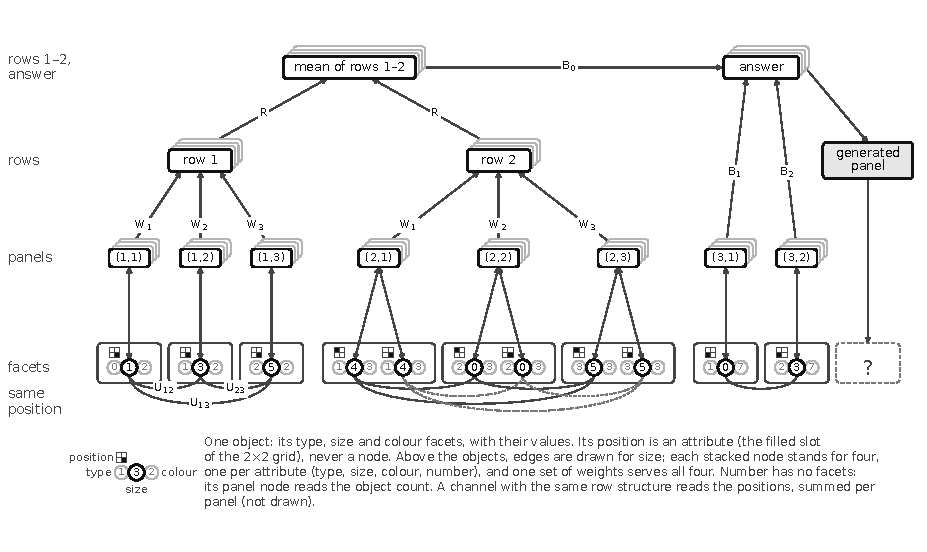
\includegraphics[width=\linewidth]{figures/facet_graph}
\caption{The facet model's graph of the puzzle in Figure~\ref{fig:iraven_puzzle}. Each object has one facet node per attribute. A facet reads its panel node and the same attribute of the objects at the same position in the other columns of its row, with one weight per pair of columns (U). A row node reads its three panels with one weight per column (W). Both complete rows reach their mean through the same weight (R), because one rule with the row as a variable writes it, and the answer reads panels (3,1) and (3,2) and that mean (B). Positions are an attribute of each object, never a node. Grounding the template on another puzzle gives another graph.}\label{fig:facet_graph}
\end{figure}

\textbf{Training.} Adam with learning rate 3·10⁻⁴, one puzzle per update, 80 epochs on the 42,000 training puzzles of all seven layouts together. The checkpoint is epoch 55.

\textbf{What the template does not name.} Every rule above has the attribute, the component, the object and the complete row as variables. By the theorem of Chapter~\ref{ch:3}, the model therefore cannot distinguish:

\begin{center}\small
\begin{tabularx}{\linewidth}{@{}YYY@{}}
\toprule
not named & so the model is unchanged by & random weights, largest change of the output \\
\midrule
objects & reordering the objects of a panel & 8·10⁻¹⁶ \\
the two complete rows & exchanging rows 1 and 2 & 3·10⁻¹⁶ \\
components & exchanging the two components (attribute outputs) & 0 \\
attributes & exchanging type and colour, with the outputs & 0 \\
candidates & reordering the candidates & 0 (they are not an input) \\
\bottomrule
\end{tabularx}
\end{center}

It does name the columns, so exchanging two columns changes the output (by 0.5 to 1.0 with random weights), as it should: Progression has a direction. It names no position slot either, but the occupancy is a vector with one entry per slot and its weights are dense, so mirror symmetries of the grids are learned and not built in.

\textbf{What is built in, stated as priors.} Objects are units, and a panel is a set of them. Attributes are independent and behave alike. Values have an order, through the thermometer code. Columns have an order. The same relation holds in every row. The objects in the same position of neighbouring panels correspond.

\section{Variants used in the experiments}\label{sec:4.5}

The experiments of Chapters~\ref{ch:6} and \ref{ch:7} change one thing at a time. These are the changes.

\textbf{A symmetry removed, in two ways} (Section~\ref{sec:6.1}).

\begin{itemize}
\item \emph{Labels.} A fact gives each component, or each attribute, a fixed one-hot vector that the rules read. The weights stay shared; the model can now tell the components apart. This adds 320 or 512 weights.
\item \emph{Separate weights.} Every rule is written once per component, or attribute, with its own weights. To keep the comparison fair this is run twice: at the same widths, which doubles or triples the weights, and at narrower widths that give the same number of weights as the shared model.
\end{itemize}

\textbf{Copy links} (Section~\ref{sec:6.5}). A direct connection from each context panel's value to the output, opened or closed by a learned gate. With \emph{per-panel gates} each of the eight panels has its own gate weights, which names the panels and gives up the symmetry between rows 1 and 2. With \emph{content gates} a gate is computed from the panel's own value with weights shared over the panels of a row, which keeps it.

\textbf{Column roles} (rows of 10). The columns of a row are first, middle and last, and the eight middle columns enter through one rule with the panel as a variable. The middle columns can then be exchanged, which is the symmetry of Arithmetic's operands. This variant has 288k weights against 1,411k for named columns, and is the model on which the attribute symmetry is removed in Sections~\ref{sec:6.2} and \ref{sec:6.3}. Section~\ref{sec:6.6} measures what the middle columns' symmetry buys.

\textbf{Two wrong symmetries} (Section~\ref{sec:6.7}). \emph{Columns tied}: columns 1 and 2 share their weights and enter symmetrically, so the model cannot tell (a, b, c) from (b, a, c). \emph{Values folded}: v and max − v get the same input code, so the model cannot tell a puzzle from its reflection. Both are exact with random weights.

\textbf{The value axis} (Sections~\ref{sec:6.2} and 7). A second template for I-RAVEN-X, built to put a symmetry on the values themselves. In the facet model a value is a code, read through one weight per bit, so ``two more than 17'' and ``two more than 33'' are different things to learn. In the value-axis template every value is a constant, \texttt{v0 … v50}, a panel's attribute is a fact \texttt{x(P, A, v17)}, and background facts \texttt{off(U, V, k)} say that V lies k steps above U. A rule

\begin{Verbatim}[fontsize=\small,breaklines]
h(P, A, V) :- x(P, A, U), off(U, V, k)        one weight per offset k
\end{Verbatim}

is then a convolution along the line of values: the same weights at every value. No rule names a value, so the template is equivariant to shifting all values, to about 10⁻¹⁶ with random weights, and a checkpoint trained on values 0–50 runs unchanged on 0–100. Its ablation writes every rule once per value with separate weights (335k weights against 10.8k), which names the values and removes the symmetry.

This template is a test bed and not a competitor of the facet model. Besides the convolution it is given features in the shape of the rules: exact running sums along a row through a background relation \texttt{plus(U, W, V)} for U + W = V, the number of distinct values in a row, and offsets from the last panel. With them it answers I-RAVEN-X puzzles almost perfectly, and that says little, since the hard part was handed to it. We therefore compare the value axis only with itself: shared weights against weights per value, and with \texttt{plus} against without. In one variant the given sums are removed and only the \texttt{plus} facts are kept, so that learned rules have to use them (Chapter~\ref{ch:7}).

\section{Baselines}\label{sec:4.6}

Every baseline is trained on the facet model's task: the same puzzles and splits, the same target description, the same loss, the same choice of epoch and the same two measures. The trainer refuses to run unless it reproduces the facet pipeline's targets on a sample of puzzles. Only the architecture differs. Each is sized to the facet model's number of weights, about 265k on I-RAVEN.

\begin{center}\small
\begin{tabularx}{\linewidth}{@{}lYY@{}}
\toprule
model & input & what it shares \\
\midrule
MLP & all context panels as one vector: per panel and slot, occupancy and the three codes & nothing \\
object GNN & one node per object, with its row, column, slot and component as labels; every node connected to every other & weights over objects \\
attribute GNN A & the facet model's graph: one node per object and attribute; nodes labelled with row, column, component, attribute and slot & weights over objects, as in B, but the labels let it tell everything apart \\
attribute GNN B & the same graph; nodes labelled only relatively: complete or question row, column, query & the facet model's symmetries: rows 1 and 2, components, attributes \\
ViT & the images of the eight context panels as one picture, cut into 16-pixel patches & weights over patches \\
ViT, rows built in & the same, with the two complete rows given as a set & also rows 1 and 2 \\
\bottomrule
\end{tabularx}
\end{center}

\textbf{A and B} are the pair that separates two things the facet model changes at once: the granularity of the graph and the symmetries. Both are written in PyTorch on the facet model's graph. B has the facet model's symmetries and A does not, so the object GNN against A measures granularity, A against B measures the symmetries, and B against the facet model measures what the lifted framework itself adds.

\textbf{The ViT} is the black-box vision reference the assignment asks for: depth 6, pre-norm blocks, at width 64 (335k weights, the closest to the facet model) and width 224 (3,753k). It generates the same description as every other model. Its target and the candidates it is matched against come from the annotation, so it is given labels for the answer and the candidates, and images for the context.

\textbf{Training.} MLP, object GNN and the attribute GNNs: AdamW, 300 epochs, with the regularisation picked on the selection puzzles from a grid of 40 runs of the MLP and the object GNN (weight decay 0.5, cosine schedule, gradient clipping; layer normalisation in the MLP). The plain versions without regularisation are reported too. The ViT uses the usual recipe for a transformer trained from scratch (learning rate 5·10⁻⁴, weight decay 0.05, cosine schedule with warm-up, dropout 0.1), not tuned here. Larger versions of the MLP and the object GNN, up to 64 times the weights, were trained to check that size is not what they lack.

\textbf{Symbolic references.} Two models mark the level reached when the rules are given: a template in which the four rules are written out as logic and only 41 weights are learned, and a solver in plain Python with nothing learned. They show what remains hard once the rules are known, and they are the only models here that see the candidates.

\textbf{What each model is given.}

\begin{center}\small
\begin{tabularx}{\linewidth}{@{}YYllY@{}}
\toprule
 & objects & rules & candidates & symmetries built in \\
\midrule
symbolic references & labels & yes & yes & – \\
facet model & labels, or the recognizer & no & no & objects, rows 1 and 2, components, attributes \\
attribute GNN B & labels & no & no & the same \\
attribute GNN A & labels & no & no & objects \\
object GNN & labels & no & no & objects \\
MLP & labels & no & no & none \\
ViT & images of the context; labels for the target & no & no & patches \\
\bottomrule
\end{tabularx}
\end{center}

\chapter{The solver: accuracy, end to end, and against the baselines}\label{ch:5}

Cells are matched \% with exact \% in brackets.

\section{I-RAVEN, test split}\label{sec:5.1}

Every model below was scored once on the 14,000 test puzzles, after its checkpoint and all settings were fixed (Section~\ref{sec:4.2}). Before its test pass each baseline checkpoint was scored again on the unseen validation puzzles and had to reproduce its recorded numbers, which all did exactly.

\begin{center}\small
\begin{tabularx}{\linewidth}{@{}YlYY@{}}
\toprule
model & weights & given & test, matched (exact) \\
\midrule
symbolic template, rules given & 41 & labels, rules, candidates & 98.3 \\
\textbf{facet model} & 267k & labels & \textbf{97.2} (68.4) \\
\textbf{facet model, end to end} & 267k + 326k & images & \textbf{97.0} (68.1) \\
attribute GNN B, the facet model's symmetries & 267k & labels & 96.8 (67.8) \\
attribute GNN A, absolute labels & 266k & labels & 95.1 (62.5) \\
object GNN, 16 times the weights & 4,258k & labels & 93.4 (63.7) \\
object GNN, 2 seeds & 265k & labels & 90.8 ± 1.2 (55.1) \\
MLP, 2 seeds & 264k & labels & 72.7 ± 1.2 (27.2) \\
ViT, width 224 & 3,753k & images of the context & 93.1 (64.4) \\
ViT, width 64 & 335k & images of the context & 78.7 (37.4) \\
ViT, rows 1 and 2 built in, width 224 / 64 & 3,709k / 323k & images of the context & 92.3 (62.4) / 89.8 (54.5) \\
\bottomrule
\end{tabularx}
\end{center}

The object GNN and the MLP are the regularised versions; without regularisation they reach 87.8 ± 1.1 and 60.8 ± 0.1.

Four things can be read from the table.

\textbf{The model generates the answers of I-RAVEN without being given the rules or seeing the candidates.} It answers 97.2\% of test puzzles, 1.1 points below the template in which the rules are written out.

\textbf{Test and validation agree.} The facet model scored 97.3 on the unseen validation puzzles and 97.2 on test; end to end, 97.1 and 97.0. No model in the table moves by more than 0.7 points between the two splits, and the order of the models is the same. The validation puzzles were looked at for weeks, and this did not inflate the numbers.

\textbf{The order follows the structure given to the model.} A flat vector of all panels gives 73\%. Objects as nodes give 91\%. One node per attribute of each object gives 95\%. The symmetries of rows, components and attributes on top of that give 97\%. Sixteen times the weights do not make up one step: the large object GNN stays below the small attribute GNN.

\textbf{Against black-box vision.} The vision transformer that reads the context images reaches 93.1\% with 3.75 million weights. The facet model behind its recognizer reaches 97.0\% with 592 thousand in total, 3.9 points more with a sixth of the weights. At a comparable size, the transformer with 335k weights reaches 78.7\%. The two pipelines are not given the same supervision: the recognizer is trained on the annotated objects of every panel, while the transformer gets the annotation of the answer only. What the comparison shows is the value of that intermediate representation together with the structure built on it, and the next sections separate the two.

\textbf{Against published solvers.} Our transformer is a plain one, not an architecture built for these puzzles. \citet{malkinski2025airaven} retrained thirteen such architectures under one protocol, on the same 6,000 training puzzles per layout, each with an auxiliary loss on the puzzle's rules. Three of the strongest, as their authors report them and as rerun:

\begin{center}\small
\begin{tabular}{@{}lll@{}}
\toprule
I-RAVEN test, 6,000 training puzzles per layout & reported & rerun under one protocol \\
\midrule
SCL & 95.0 & 83.4 \\
PredRNet & 96.5 & 88.8 \\
DRNet & 97.6 & 90.9 \\
our vision transformer, width 224 &  & 93.1 \\
facet model, end to end &  & 97.0 \\
\bottomrule
\end{tabular}
\end{center}

These models pick one of the eight candidates. Ours generate the answer, and matched accuracy counts it right when the closest candidate is the answer, so the two scores are close but are not the same task. The rerun models also learn from the labels of the rules, which ours never see. Within those limits our transformer is a fair stand-in for black-box vision at this amount of data, not a weak one.

\section{By layout}\label{sec:5.2}

Matched \% on test.

\begin{center}\small
\begin{tabular}{@{}llllllll@{}}
\toprule
model & centre & 2×2 & 3×3 & left-right & up-down & in-out & in-out grid \\
\midrule
symbolic template, rules given & 99.9 & 96.0 & 95.5 & 100.0 & 100.0 & 99.9 & 97.3 \\
facet model & 99.6 & 95.0 & 89.1 & 99.8 & 99.7 & 99.8 & 97.5 \\
facet model, end to end & 99.6 & 95.0 & 89.1 & 99.8 & 99.7 & 99.8 & 96.4 \\
attribute GNN B & 99.8 & 95.2 & 85.5 & 100.0 & 99.9 & 99.7 & 97.5 \\
attribute GNN A & 99.9 & 89.5 & 84.4 & 100.0 & 99.9 & 100.0 & 92.0 \\
object GNN, 16× & 99.8 & 88.2 & 74.5 & 99.8 & 99.8 & 99.8 & 92.2 \\
MLP, seed 0 & 94.4 & 46.4 & 38.8 & 91.2 & 87.1 & 95.3 & 61.6 \\
ViT, width 224 & 99.1 & 92.8 & 80.5 & 99.8 & 99.6 & 99.8 & 80.0 \\
\bottomrule
\end{tabular}
\end{center}

Every model except the MLP solves the four layouts whose components hold a single object. The differences are in the grids. The 3×3 grid is the hardest layout for every learned model, the facet model included: it loses 6.4 points there to the rules-given template, and less than one point on any other layout. The vision transformer loses most on the 3×3 grid and the in-out grid. Training it on the grid layouts alone, with finer patches or larger images, did not help; it memorised (training loss near zero, selection accuracy 33–36\%). The same grid puzzles were learned once the single-object layouts were added to the training set, so at this amount of data the transformer needs the easy layouts to find the task at all.

\section{End to end}\label{sec:5.3}

Replacing the annotation by the recognizer costs 0.16 points on test (97.19 to 97.03), and 0.18 on the validation puzzles. All of it falls on the in-out grid, the one layout the recognizer misreads; the other six layouts are unchanged to the puzzle.

\begin{center}\small
\begin{tabular}{@{}lll@{}}
\toprule
test puzzles & share & matched \\
\midrule
all 16 panels read right & 95.6\% & 97.2 \\
at least one panel misread & 4.4\% (611 puzzles) & 92.6 \\
\bottomrule
\end{tabular}
\end{center}

A misread panel is usually not fatal. The model still matches 92.6\% of the puzzles in which the recognizer made an error, because one wrong value among eight panels moves the generated description a little, and the right candidate often stays the closest.

For comparison, the rules-given template loses 2.0 points behind an earlier recognizer, a ResNet-18 that reads all 16 panels right in 92.6\% of puzzles.

One limit was found here. The facet template has no bias terms and normalises its facet vectors, and value 0 is the code with no bit on. A code of 10⁻⁶ in place of 0 is therefore rescaled to full size and read as a large value. The model cannot take graded inputs as it stands, which is why the recognizer's uncertainty is not passed on (Section~\ref{sec:4.3}). Training the two parts jointly would need this changed first.

\section{By amount of training data}\label{sec:5.4}

The models were retrained on the first 300, 1,000 and 3,000 puzzles of every layout, with the number of updates kept the same. These runs were scored on the unseen validation puzzles only, with one seed. The relational models read the annotation. The facet model was also run end to end: the recognizer of Section~\ref{sec:4.3} was trained from scratch on the same first puzzles of every layout, and the facet checkpoint of that size read its panels (at 6,000 puzzles it is the recognizer of Section~\ref{sec:5.3}, trained on 2,000).

\begin{center}\small
\begin{tabularx}{\linewidth}{@{}YlllllllY@{}}
\toprule
training puzzles per layout & facet & facet, end to end & GNN B & GNN A & object GNN & MLP & ViT 224 & ViT 224, rows built in \\
\midrule
300 & 90.0 (53.3) & 89.8 (53.1) & 87.0 (53.0) & 86.1 (50.8) & 29.6 (1.1) & 24.9 (0.5) & 15.6 (0.2) & 14.6 (0.1) \\
1,000 & 94.1 (62.7) & 93.9 (62.4) & 93.9 (64.0) & 93.4 (61.5) & 68.7 (21.9) & 48.1 (7.7) & 18.6 (0.2) & 23.8 (0.5) \\
3,000 & 96.1 (66.0) & 95.8 (65.7) & 96.8 (68.8) & 95.9 (65.3) & 86.5 (49.8) & 64.5 (19.1) & 45.8 (4.5) & 62.0 (13.3) \\
6,000 & 97.3 (69.1) & 97.1 (68.8) & 96.8 (67.9) & 95.0 (62.5) & 90.5 (55.1) & 72.0 (27.5) & 93.4 (64.4) & 92.1 (62.1) \\
\bottomrule
\end{tabularx}
\end{center}

\textbf{Reading the panels costs little at any size.} End to end the facet model loses 0.2 to 0.3 points at every size, almost all of it on the in-out grid, the layout the recognizer misreads most. Trained on 300 puzzles per layout the recognizer reads all 16 panels of a puzzle right in 90\% of puzzles, and on 3,000 in 96\%. Where it misreads a panel the facet model still answers 78\% of those puzzles at 300 and 89\% at 3,000.

\textbf{The gap is largest when data is scarce.} From 300 puzzles per layout the facet model answers 90\% end to end and the vision transformer 16\%, barely above the 12.5\% of guessing. The transformer needs twenty times the puzzles to pass the facet model's score at 300. This is the comparison the assignment asks for: 4 points at 6,000 puzzles, 74 at 300.

\textbf{The two do not learn from the same labels.} The recognizer is trained on the labelled objects of all 16 panels of every training puzzle, the transformer on the answer's index alone. The end-to-end curve removes the annotation at test time, not its help in training. The 74 points therefore measure what an object-level representation, together with the labels it is trained from, is worth against learning the whole task from the answer; they are not a contest between two pixel learners on the same supervision. A transformer first trained to read the same object labels and then on the answer would separate the two, and was not run.

\textbf{Most of that gap is the representation.} At 300 puzzles the three models on the attribute graph have 86 to 90\% and the object GNN has 30\%, with the same labels as input. The step from a node per object to a node per attribute is worth more than 56 points there. The symmetries are worth 1 to 4 points among the three attribute models. On I-RAVEN, then, the graph carries the result and the symmetries refine it. Chapter~\ref{ch:6} shows where symmetries carry more: on values, and on what the training data never showed.

\section{The symmetries carry the result, not the framework}\label{sec:5.5}

The attribute GNN B is written in PyTorch and has the facet model's symmetries. It reaches 96.8\% on test against the facet model's 97.2\%, and stays within 3 points of it at every amount of data, ahead at 3,000. The 0.4 points on test are one run each; two seeds of the object GNN differ by 1.7. We therefore do not claim that the lifted framework makes a model more accurate. By layout, the facet model's lead is the 3×3 grid (89.1 against 85.5), and the two are within 0.2 points everywhere else.

What the template contributes is of another kind. The symmetries of B had to be engineered into its node labels and checked one by one. In the template they follow from which constants are left unnamed, one proof covers all of them, and removing one is a change of a line (Chapter~\ref{ch:6}).

\section{Where the facet model fails}\label{sec:5.6}

\textbf{Not on a particular rule.} It matches 97.3\% of the validation puzzles that contain an Arithmetic rule and 97.3\% of those that do not. Generating type, size and colour exactly, by the rule the attribute follows:

\begin{center}\small
\begin{tabular}{@{}lllll@{}}
\toprule
 & Constant & Progression & Distribute Three & Arithmetic \\
\midrule
facet model & 83.7 & 89.7 & 88.7 & 83.8 \\
ViT, width 224 & 82.4 & 89.7 & 86.6 & 86.3 \\
\bottomrule
\end{tabular}
\end{center}

Constant is the lowest because of the grids, where panels that are not uniform hold noise values (Section~\ref{sec:4.1}).

\textbf{On number and position.} When the number of objects in a grid changes along the row, the model generates the right count in 44 to 49\% of cases and the right positions in 51 to 71\%. This is why exact is 68\% where matched is 97\%: the candidates rarely differ in these, so matching does not need them. It is also the place where the rules-given template gains its 6 points on the 3×3 grid. Position rules are set operations and cyclic shifts over slots, and the facet model's position channel has none of that structure.

\section{I-RAVEN-X}\label{sec:5.7}

On I-RAVEN-X with rows of 3 and values 0–10 the plain facet model reaches 99.2 (97.0), with 95.0\% of Arithmetic values exact.

With rows of 10 the picture changes, and we report it without a ranking. The plain model reaches 87.4 ± 1.8\% matched at values 0–50 over three seeds and generates 18.4 ± 3.0\% of answers exactly; Arithmetic values are exact in 20.7 ± 2.2\% of cases. Variants that build in more raise this: with column roles, 94.2 ± 0.2 (27.6 ± 2.0) and 39.6 ± 1.3\% on Arithmetic, with a fifth of the weights (36.0 ± 2.1\% on Arithmetic on the test range, scored once at the end; Appendix~\ref{sec:D.6}). A torch attribute GNN B trained for seven times as many epochs without regularisation reaches 97.9 (45.5) and 98.2 (56.5) in two seeds, level with the best facet variant. These runs differ in training length and recipe, most have one seed, and the baselines' recipe was tuned on I-RAVEN, so they do not support an order of models, and we give none. What they do support: no model that has to learn sums generates more than about half of the Arithmetic values exactly on rows of 10, and matching hides this. Rows of 10 are used in the rest of the thesis for experiments inside one model family, where only one thing changes.

\section{Cost}\label{sec:5.8}

The lifted approach has a real cost. PyNeuraLogic grounds every puzzle into its own network and keeps all of them in memory, and it updates the weights one puzzle at a time, on CPU.

\begin{center}\small
\begin{tabular}{@{}lll@{}}
\toprule
run & peak memory & time \\
\midrule
facet model with content gates, I-RAVEN, all layouts & 327 GB & 15 h \\
facet model with copy links, rows of 10, values 0–1000 & 344 GB & 16 h \\
value axis with \texttt{plus} in learned rules, rows of 10 & 104–161 GB & 3–7 h \\
\bottomrule
\end{tabular}
\end{center}

Grounding takes 10 to 165 ms per puzzle and is done once; an epoch over all of I-RAVEN takes about 14 minutes. The torch baselines of the same size train on one GPU in a few gigabytes. Scoring is cheap by comparison: the whole test split, with labels and end to end, took 15 minutes and 16 GB.

\chapter{What a symmetry buys and what a wrong one costs}\label{ch:6}

Cells are matched \% with exact \% in brackets, on unseen puzzles, one seed unless marked.

Chapter~\ref{ch:5} compared models that differ in many things at once. This chapter changes one symmetry at a time inside one model, and compares each outcome with what Chapter~\ref{ch:3} predicts. The predictions, in the order of the sections:

\begin{enumerate}
\item A symmetry the data has merges inputs that need the same answer. A model with it built in has fewer things to learn, by a factor of up to the size of the group. The gain should be largest when training puzzles are few, grow with the group, and disappear once the training set covers every case by itself.
\item That gain comes from sharing weights. A model that shares them but is not exactly invariant should lose nothing on puzzles like the training ones.
\item Exact invariance matters where the data cannot teach the symmetry: on inputs the training set never contained, and where the generator leaves a gap between what is valid and what it produces. A symmetry of the task in that gap costs nothing on the right solution, and where the rule itself ignores what the symmetry exchanges, it helps that rule even at full data.
\item A symmetry that leads out of the data sets no ceiling. One that maps valid puzzles onto valid puzzles with another answer sets a ceiling that can be counted in advance, and data does not lift it.
\end{enumerate}

\section{Design}\label{sec:6.1}

Each experiment trains the same template twice or more on the same puzzles: with the symmetry, and with it removed in one of the ways of Section~\ref{sec:4.5}. \emph{Labels} keep all weights shared and let the model tell the things apart. \emph{Separate weights} give each component, attribute or value its own copy of every rule. The separate-weight models are run at the same number of weights as the shared model, by narrowing them, so that a difference is not a difference in size. Every run takes the same number of updates.

Three symmetries are tested in Sections~\ref{sec:6.2} and \ref{sec:6.3}, each a symmetry of the data it is tested on (Section~\ref{sec:3.5}):

\begin{center}\small
\begin{tabularx}{\linewidth}{@{}YYYY@{}}
\toprule
symmetry & group & model & data \\
\midrule
the two components & 2 elements & facet model & I-RAVEN, left-right and up-down layouts \\
the attributes & size and colour exchangeable; type for three of four rules & facet model, column roles & I-RAVEN-X, rows of 10, values 0–50 \\
a shift of all values & about 50 elements & value axis, rules' primitives given & I-RAVEN-X, rows of 10, values 0–50 \\
\bottomrule
\end{tabularx}
\end{center}

\section{A symmetry the data has saves training data}\label{sec:6.2}

\begin{center}\small
\begin{tabularx}{\linewidth}{@{}lYYYl@{}}
\toprule
symmetry & training puzzles & built in & removed, same number of weights & gain \\
\midrule
components & 100 per layout, 3 seeds & 88.0 ± 1.9 (42.4 ± 3.0) & 73.8 ± 1.4 (19.4 ± 1.4) & \textbf{+14.2 ± 1.9} \\
 & 1,000 & 99.3 (95.6) & 98.5 (84.5) & +0.8 \\
 & 6,000 & 99.9 (97.7) & 100.0 (98.8) & −0.1 \\
attributes & 600, 3 seeds & 66.2 ± 2.7 (13.3 ± 2.8) & 52.7 ± 0.7 (3.6 ± 0.0) & \textbf{+13.5 ± 2.1} \\
 & 6,000, 3 seeds & 94.2 ± 0.2 (27.6 ± 2.0) & 87.9 ± 1.6 (15.4 ± 2.7) & +6.3 ± 1.7 \\
value shift & 100 & 99.0 (97.3) & 38.3 (4.0) & \textbf{+60.7} \\
 & 600 & 99.9 (99.9) & 92.7 (81.0) & +7.2 \\
 & 6,000 & 100.0 (100.0) & 98.4 (97.4) & +1.6 \\
\bottomrule
\end{tabularx}
\end{center}

The gains with three seeds are the means of the gains per seed; each seed's gain is within one standard deviation of the mean (components 12.0 to 15.4, attributes 11.5 to 15.7 at 600 and 4.8 to 8.1 at 6,000). The value-shift rows are not at equal size: the shared model has 10.8k weights and the model with weights per value 335k, because a copy of every rule is needed for each of 51 values.

\textbf{The gain is largest with little data and shrinks as data grows}, in all three cases. For the components it is gone at 6,000 puzzles: by then the training set shows each component every rule often enough.

\textbf{The gain grows with the group.} A group of two buys 14 points at 100 puzzles. The shift of about fifty values buys

\begin{enumerate}
\item Put as data, the model without the value shift is still behind after sixty times the puzzles: 98.4\% at 6,000
\end{enumerate}

against 99.0\% at 100. That factor is more than sixty, larger than the group, but the two models also differ thirty times in size, so it is not the symmetry's alone. The direction is consistent with the sample-complexity results of Section~\ref{sec:2.4}. The size of the saving we counted only where the models are otherwise equal, next.

\textbf{The saving, counted in puzzles before the runs.} Section~\ref{sec:2.4} cites proofs, for kernel methods, that a symmetry saves data by a factor of up to the size of its group. For the components the factor can be read from the template. Each training sample is one component of one puzzle. With separate weights the copy for one component trains only on that component's samples, while the shared network trains on both. The two components follow the same distribution, so a separate model given twice the puzzles gives each copy what the shared network gets: the factor is exactly 2. For the components this count is close to a tautology. What the run tests is that nothing else is at work: neither a gain the shared network draws from serving both components, nor a loss from it. For the attributes it is not one number. Size and colour carry the four rules equally often, but type never carries Arithmetic. The shared network therefore sees twice the examples a separate copy sees on Arithmetic, and up to three times on the other rules. We wrote these predictions down, then trained the separate model at the same widths as the shared one on twice and three times the data:

\begin{center}\small
\begin{tabularx}{\linewidth}{@{}YlYYl@{}}
\toprule
symmetry, puzzles scored & shared weights & separate weights, more data & predicted & measured \\
\midrule
components, all & 100: 88.0 ± 1.9 & 200: 88.1 ± 0.2 & equal (factor 2) & equal \\
attributes, with Arithmetic & 600: 63.0 ± 2.9 & 1,200: 60.8 ± 1.2 & equal (factor 2) & within 2.2 points \\
attributes, without Arithmetic & 600: 68.7 ± 2.8 & 1,200: 64.0 ± 0.8 & separate behind (factor above 2) & 4.7 behind \\
attributes, all & 600: 66.2 ± 2.7 & 1,200: 62.6 ± 0.6; 1,800: 69.8 ± 0.9 & between the two (factor 2 to 3) & between the two \\
\bottomrule
\end{tabularx}
\end{center}

Three seeds each, matched \%. On the components, where the count is nearly a tautology, it holds to a tenth of a point: the shared network draws nothing from serving both components beyond the doubled data. The attributes are the real test, because there the count is not the size of the group, and the pattern is the counted one. At twice the data the gap closes where only size and colour teach the rule, and stays where type also does; at three times the data the separate model is level on the puzzles without Arithmetic (69.8 against 68.7) and ahead on those with it. The attributes are worth between two and three times the data, about two and a half, which is what the count of examples allowed. Built-in sharing is worth the training data it reuses, and no more. Figure~\ref{fig:data_factor} shows both comparisons. The same checkpoints scored once on the test range at the end of the work give the same reading: separate weights at 200 puzzles 88.3 ± 0.6 against shared at 100 88.4 ± 1.3, and on attributes shared at 600 (68.3) between separate at 1,200 (65.0) and 1,800 (72.3) (Appendix~\ref{sec:D.6}).

\begin{figure}[tbp]
\centering
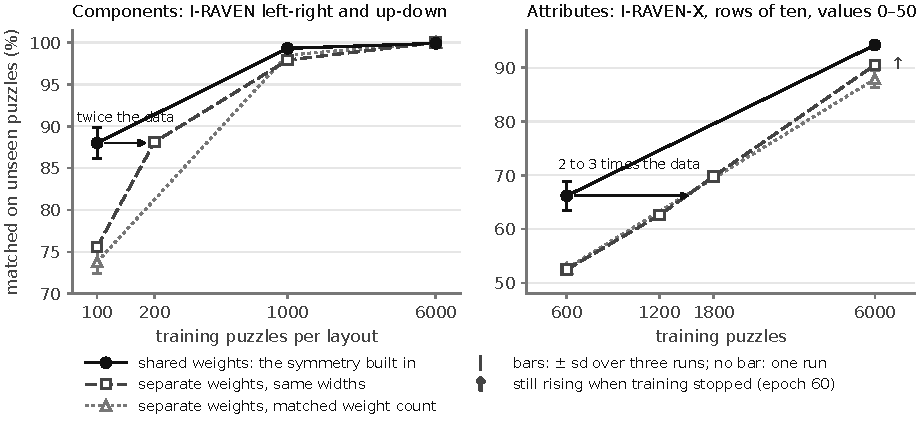
\includegraphics[width=\linewidth]{figures/data_factor}
\caption{What a symmetry is worth in training data. Matched \% on unseen puzzles against the number of training puzzles, for the facet model with one set of weights shared by the two components or by the three attributes, and with separate weights, at the same widths or at a matched weight count. Without the symmetry the model needs twice the data for the components and two to three times for the attributes, as counted before the runs. Bars: one standard deviation over three seeds.}\label{fig:data_factor}
\end{figure}

\textbf{Giving the removed-symmetry models their full width does not help them.} At the same widths as the shared model, with two to three times the weights, they score 75.6 on components at 100 puzzles and 52.5 on attributes at 600, within a point of the narrowed versions.

\textbf{The same holds in a model that is not relational.} Giving the vision transformer the two complete rows as a set builds in the exchange of rows 1 and 2. At 3,000 puzzles per layout this raises the small transformer from 48.2 to 68.2 (means of three seeds; the gain per seed is 8.6 to 28.0 points) and the large one from 45.8 to 62.0 (one seed). At 6,000 the small one keeps a gain of 10 points and the large one none (92.1 against 93.4). Below 3,000 neither version learns the task, so there is nothing for the symmetry to multiply.

\section{The gain is the sharing, not the exact invariance}\label{sec:6.3}

Labels remove the invariance and keep the sharing. With random weights, a labelled model changes its output by 0.4 when the components are mirrored. Trained, it does as well as the exactly invariant model:

\begin{center}\small
\begin{tabularx}{\linewidth}{@{}llYYY@{}}
\toprule
 & training puzzles & exactly symmetric & labels, weights shared & separate weights \\
\midrule
components & 100, 3 seeds & 88.0 ± 1.9 & 89.5 ± 2.1 & 73.8 ± 1.4 \\
 & 1,000 & 99.3 & 99.6 & 98.5 \\
attributes & 600, 3 seeds & 66.2 ± 2.7 & 64.8 ± 2.1 & 52.7 ± 0.7 \\
 & 6,000 & 94.2 ± 0.2 (3 seeds) & 93.9 & 87.9 ± 1.6 (3 seeds) \\
\bottomrule
\end{tabularx}
\end{center}

The reason is visible in the template. A labelled model adds a few hundred weights for the labels and keeps every other weight in a rule that serves both components, so every training puzzle still trains every weight. And because the two components follow the same distribution, nothing in the data rewards treating them differently: the trained labelled models change by at most 0.8 points when a puzzle is mirrored, and by at most 1.1 when size and colour are exchanged. Per seed, labels score 1.4 ± 0.8 points above the symmetric model on components and 1.3 ± 0.7 below it on attributes. They have learned the symmetry they were not given.

The same comparison exists in PyTorch. Attribute GNN A is B with absolute labels on its nodes. On I-RAVEN it trails B by 0.5 to 1.8 points at every amount of data (Section~\ref{sec:5.4}), which is the distance between two seeds.

So on puzzles like the training ones, a data symmetry pays through weight sharing, and exactness adds nothing measurable. The next two sections are the cases where it does.

\section{What training never showed}\label{sec:6.4}

\textbf{An attribute that never carried a rule.} We removed from training and selection every puzzle in which size follows Progression, and scored how often the size is generated exactly on unseen puzzles that have this pair.

\begin{center}\small
\begin{tabularx}{\linewidth}{@{}YlY@{}}
\toprule
model & pair held out & pair in training (3,000 puzzles) \\
\midrule
facet model & \textbf{87.7} & 89.9 \\
attribute GNN B, symmetric & \textbf{84.1} & 89.4 \\
attribute GNN A, the same with labels & 42.3 & 85.9 \\
object GNN & 20.6 & 83.2 \\
MLP & 19.7 & 68.0 \\
ViT, width 224 & 18.5 & 48.9 \\
\bottomrule
\end{tabularx}
\end{center}

The models that cannot tell size from colour apply to size what they learned about Progression on colour and type, and lose 2 to 5 points. The labelled model A, which matched B everywhere in Section~\ref{sec:6.3}, loses 44. The data could teach A that the attributes behave alike only where it showed them behaving alike. Here exact invariance is the whole difference between two models with the same sharing.

\textbf{A layout that was never trained.} Trained on six layouts without up-down and scored on up-down:

\begin{center}\small
\begin{tabular}{@{}lllllll@{}}
\toprule
 & facet & GNN B & GNN A & object GNN & ViT 224 & MLP \\
\midrule
matched on up-down & 99.1 & 99.5 & 99.9 & 23.6 & 14.0 & 13.3 \\
\bottomrule
\end{tabular}
\end{center}

All three models on the attribute graph answer the unseen layout as well as a trained one, and the others are near the 12.5\% of guessing. Labelled A transfers as well as the symmetric models, so this is not an effect of exact symmetry. It comes from the graph: on it an object's type, size and colour are processed without reference to the slot the object sits in, and up-down differs from the trained left-right layout only in its slots. Exact generation is 0 for every model on this layout, because the output bits for its two slots were never trained.

\textbf{Values that were never trained.} The value-axis model has no weight that belongs to a value. A checkpoint trained on values 0–50 was run on puzzles with values 0–100 and scores 100.0 (100.0); trained on 100 puzzles, 98.1 (96.8). The version with weights per value cannot be run on the wider range at all, and neither can any model that reads thermometer codes.

\section{A symmetry given up lets a shortcut in}\label{sec:6.5}

On rows of 10, exchanging rows 1 and 2 is a symmetry of the task but not of the data: the exchanged puzzle has the same answer and the generator never produces it (Section~\ref{sec:4.2}). The training data therefore cannot teach it, and a model without it is free to learn something that holds only on what the generator produces.

Copy links show this. They let the model pass a context panel's value straight to the output, which suits Constant and Distribute, whose answers are values of the context. With a gate per panel, the model can tell the panels apart.

\begin{center}\small
\begin{tabularx}{\linewidth}{@{}YYY@{}}
\toprule
I-RAVEN-X, rows of 10, values 0–50 & as generated & rows 1 and 2 exchanged \\
\midrule
copy links, a gate per panel & \textbf{97.8} & about 60 \\
copy links, gates computed from content & 94.9 & 94.9, identical \\
plain facet model & 87.4 ± 1.8 (3 seeds) & identical \\
\bottomrule
\end{tabularx}
\end{center}

The model with a gate per panel has the highest score on the generated puzzles and loses 38 points when the rows are exchanged. On puzzles with a Distribute attribute it falls from 98.3 to 39.5. In the generated data a Distribute row is the first row moved by one step, so the value that the third row lacks always stands at the same place in the first two, and the gates learned to fetch it from that address. They did not learn the rule. Gates computed from the content of a panel cannot name an address; that model gives up 2.9 points on the generated puzzles and answers the exchanged ones identically.

The gain of copy links is real information and not just extra connections: a control with the same links wired to the wrong puzzle's panels gains 1.9 points where the proper links gain 12.4.

The baselines repeat the pattern, and they show the role of the gap.

\begin{center}\small
\begin{tabularx}{\linewidth}{@{}YYY@{}}
\toprule
matched, as generated → rows exchanged & I-RAVEN (a data symmetry) & rows of 10 (a task symmetry only) \\
\midrule
attribute GNN B, symmetric & identical & identical \\
attribute GNN A & 95.0 → 95.0 & 95.0 → \textbf{55.5} \\
object GNN & 91.3 → 91.3 & 84.0 → \textbf{52.7} \\
MLP & 72.8 → 72.4 & 84.4 → \textbf{47.7} \\
ViT, width 64 & 79.1 → 78.9 & 52.9 → \textbf{38.5} \\
\bottomrule
\end{tabularx}
\end{center}

On I-RAVEN no model needs the symmetry built in, because the data has it and teaches it. On rows of 10 every model without it fails the exchange. Model A's exact score on Distribute falls from 59.9 to 1.0: its lead over B on the generated puzzles was the same shortcut.

A benchmark score, then, does not tell a rule from a regularity of the generator. Building in a symmetry of the task that the generator lacks closes the gap between the two, at a small cost on the benchmark.

\section{A symmetry of the task that buys accuracy at full data}\label{sec:6.6}

On I-RAVEN-X with rows of 10, an Arithmetic row is a sum: its last value is the sum of the nine before it, or its first value is the sum of the nine after it. The middle columns are interchangeable operands. Exchanging two of them keeps the row valid with the same answer, and it keeps the answer of a Distribute row too, which is the value the row lacks whatever the order. But the generator never produces most of the exchanged rows: it draws the operands one after another from a shrinking range and places the zeros among them in a fixed pattern (Section~\ref{sec:3.5}). So the exchange is a symmetry of the task outside the support of the data, like the exchange of rows in Section~\ref{sec:6.5}.

The plain facet model names every column and gives each of the ten its own weights. \emph{Column roles} name only the first and the last column and read the eight middle columns through one rule, with the panel as a variable (Section~\ref{sec:3.3}). Any exchange of middle columns is then built in. Progression rows do not survive the exchange, but their answer can still be computed from the first value and the middle values taken together, so the symmetry costs Progression no answer. \emph{Prediction, written before the run:} Arithmetic improves, and nothing else loses.

\begin{center}\small
\begin{tabular}{@{}lll@{}}
\toprule
rows of 10, 6,000 puzzles, 3 seeds & named columns & column roles \\
\midrule
matched & 87.4 ± 1.8 & \textbf{94.2 ± 0.2} \\
exact, Arithmetic & 20.7 ± 2.2 & \textbf{39.6 ± 1.3} \\
exact, Distribute & 11.3 ± 1.3 & 22.9 ± 0.8 \\
exact, Progression & 86.0 ± 7.5 & 92.8 ± 1.6 \\
exact, Constant & 95.8 ± 2.5 & 97.5 ± 2.8 \\
matched, two middle columns exchanged & 71.1 ± 1.0 & identical \\
weights & 1,411k & 288k \\
\bottomrule
\end{tabular}
\end{center}

Arithmetic's exact score doubles, as predicted, and Distribute's doubles as well, which fits a rule whose answer does not depend on the order. On the test range, scored once at the end, the gain is smaller: Arithmetic 36.0 ± 2.1 against 20.9 ± 0.5, an increase of 1.7 times rather than 1.9, while matched (93.7, 94.5, 94.7 against 87.1 ± 2.0) and Distribute (21.6 against 10.5) hold (Appendix~\ref{sec:D.6}). The drop is within the sampling error of the 507 Arithmetic rows that all three seeds share, but it is the direction a choice made with those puzzles in view would leave, and column roles were chosen that way, so the test number is the safer one to quote. Progression and Constant move within the spread of the seeds. The named model loses 16 points when two middle columns are exchanged: it reads the order that the generator imposes. The roles model also has a fifth of the weights, so the size of the model could be the cause. It is not: at equal size, with widths 64, 144 and 288 and 1,390k weights, the roles model matches 94.9 (one run).

This is the largest gain from a symmetry at 6,000 puzzles in this chapter, 6.8 ± 1.6 points per seed. The data could not have taught it, because the exchanged orders never occur. Arithmetic stays the weak rule all the same: fewer than half of its values are generated exactly.

\section{A wrong symmetry}\label{sec:6.7}

Two symmetries the data does not have were built into the facet model, exactly, on I-RAVEN-X with rows of 3 and values 0–10. The predictions were written down before the runs.

\textbf{Columns 1 and 2 tied: out of the data.} The model cannot tell (a, b, c) from (b, a, c). For Constant and Distribute rows, and for sums, the exchanged row is valid with the same answer, so for them the tie is a correct symmetry. For Progression and for differences the exchanged row never occurs. Nowhere does the tie ask for two different answers to one input. \emph{Prediction:} no ceiling; at most a cost in data.

\begin{center}\small
\begin{tabularx}{\linewidth}{@{}YYY@{}}
\toprule
exact, Constant / Progression / Distribute / Arithmetic & 6,000 puzzles & 600 puzzles \\
\midrule
plain (matched 99.2 and 95.1) & 99.6 / 99.5 / 99.3 / 95.0 & 99.6 / 99.3 / 89.2 / 76.2 \\
columns 1 and 2 tied (matched 98.6 and 92.1) & 99.6 / 100.0 / 96.3 / 89.9 & 99.6 / 99.5 / 94.7 / 62.4 \\
\bottomrule
\end{tabularx}
\end{center}

No ceiling appears: the tied model matches 98.6\% at 6,000 puzzles, and Progression, whose rows the tie breaks, is generated exactly every time. The cost is on Arithmetic, 5 points at 6,000 puzzles and 14 at 600. Distribute gains 5 points at 600 puzzles, as a rule for which the tie is a correct symmetry should.

\textbf{Values folded: in conflict with the data.} The values v and 10 − v get the same input code. A puzzle and its reflection are then one input, both occur equally often, and their answers differ unless the answer is the middle value. \emph{Prediction, counted on the data:} at most 54.4\%, 56.0\% and 55.0\% of Constant, Progression and Distribute values can be exact. Arithmetic rows do not survive reflection, so they have no forced ceiling.

\begin{center}\small
\begin{tabular}{@{}lll@{}}
\toprule
 & 600 puzzles & 6,000 puzzles \\
\midrule
plain, matched & 95.1 & 99.2 \\
values folded, matched & 39.7 & 46.6 \\
values folded, values exact (type / size / colour) & 57 / 52 / 49 & 52 / 53 / 50 \\
\bottomrule
\end{tabular}
\end{center}

The folded model generates about half of all values exactly, at the counted ceiling to within the noise of a thousand puzzles. Ten times the data moves it from 49–57\% to 50–53\%, which is no movement. A plain model with a tenth of the data is far ahead of it.

\section{Summary}\label{sec:6.8}

\begin{center}\small
\begin{tabularx}{\linewidth}{@{}YYY@{}}
\toprule
what the symmetry does to valid puzzles & prediction & measured \\
\midrule
maps them to equally likely puzzles with the corresponding answer & saves data, by up to the size of the group; nothing at full data & +14 (group of 2, 3 seeds) to +61 points (about 50) at 100 puzzles; −0.1 to +6 at 6,000; counted: without the components' symmetry exactly twice the puzzles (88.1 at 200 against 88.0 at 100) \\
the same, but the model only shares weights and is not invariant & no loss on puzzles like the training ones & within 1.5 points of the invariant model (3 seeds) \\
 & a loss on what training never showed & 42.3 against 84.1 on a held-out rule and attribute \\
maps them to valid puzzles the generator never produces & no loss on the right solution; closes a shortcut & 94.9 unchanged against 97.8 → 60 under the exchange \\
 & where the rule ignores the order, a gain on that rule & Arithmetic exact 39.6 against 20.7 (test: 36.0 against 20.9); matched 94.2 against 87.4 at 6,000 (3 seeds) \\
maps them out of the valid puzzles & no ceiling, a cost in data & 98.6 against 99.2 at 6,000; 92.1 against 95.1 at 600 \\
maps them to valid puzzles with another answer & a ceiling, counted in advance & about half of the values, at 600 puzzles and at 6,000 \\
\bottomrule
\end{tabularx}
\end{center}

Every row came out on the side predicted. The sizes are single runs, and Chapter~\ref{ch:8} lists what that leaves open. The next chapter tests the first and the last row of this table on one model with two rules, where the prediction is a number.

\chapter{One model, two rules: sum and midpoint}\label{ch:7}

Cells are exact \% on the tested rule, on unseen puzzles, about 500 rows per cell. Sum and midpoint at 100 and 600 puzzles have three seeds for the shared, per-value and \texttt{plus} models, and so do the models of Section~\ref{sec:7.7}; every other cell is one run, so roughly ±4 points.

Chapter~\ref{ch:6} found that a symmetry saves data when the data has it and caps the model when it conflicts. Those were different symmetries in different models. This chapter holds the model fixed and changes only the rule, with two rules built to be alike in everything but one property. The one built-in symmetry then saves most of the data on one rule and caps the model on the other, and both amounts are computed before training.

The question came from the benchmark. Arithmetic is the rule every model that learns from data finds hardest on I-RAVEN-X (Section~\ref{sec:5.7}). Is that because a sum is a hard function, because its table is large, or because the models lack the right symmetry for it?

\section{Two rules of one form}\label{sec:7.1}

Take a row (a, b, c) of values between 0 and 50.

\begin{center}\small
\begin{tabularx}{\linewidth}{@{}YlY@{}}
\toprule
 & sum & midpoint \\
\midrule
rule & c = a + b & c = (a + b) / 2 \\
rows in the table & 1,225 (a, b ≥ 1) & 1,250 (a ≠ b, a + b even) \\
exchange of a and b keeps the row valid & yes & yes \\
adding s to all three keeps the row valid & \textbf{no} & \textbf{yes} \\
\bottomrule
\end{tabularx}
\end{center}

Both are rules of the form c = pa + qb. Both have a table of about 1,250 rows, and both are symmetric in their operands. They differ in one algebraic property. Adding the same number s to every value turns (a, b, c) into (a + s, b + s, c + s), and the rule c = pa + qb still holds for it exactly when p + q = 1 (Section~\ref{sec:2.4}). Midpoint has p + q = 1, sum has p + q = 2. In words: midpoint needs only the differences between values, and sum needs to know where zero is. Of the benchmark's rules, Constant, Progression and Distribute Three survive the common shift as well; Arithmetic is the only one that does not.

It would be wrong to say that sum has no symmetry. The rows of any rule c = pa + qb stay valid under the moves (s₁, s₂, p·s₁ + q·s₂): for sum, one operand may move if the answer moves with it. The two rules have equally many such moves. What separates them is whether the common shift (s, s, s) is among them.

\textbf{The puzzles.} We generated I-RAVEN-X puzzles with rows of 3 and values 0–50 in which Arithmetic is replaced by a test rule, and everything else is kept: the other three rules, the attributes, the splits. Two further rules guard the comparison. \emph{Mirror}, c = 2a − b, uses midpoint's triples with the columns moved; it keeps the common shift, and unlike midpoint its answer lies outside its operands, as a sum's does. \emph{Lookup}, b = g(a) and c = g(b) for a fixed random table g, has no symmetry at all and only 51 rows.

\section{The models}\label{sec:7.2}

\textbf{Shared.} The value-axis template of Section~\ref{sec:4.5} with a kernel over the whole range, closed into a ring so that the ends of the range are not special, and without \texttt{plus}. It has 14,785 weights and is exactly equivariant to the common shift: with random weights, shifting the input moves the output by the same amount to 7·10⁻¹⁷.

\textbf{Per value.} The same template with a separate copy of every rule for each value: 459,635 weights and no symmetry on the values.

\textbf{The shared model's forward pass.} For one attribute, \(x_p\) is panel \(p\)'s value and \(v\) runs over the ring of 101 values. The kernel has one learned vector \(w_k\) for each offset \(k\) from −50 to 50. A row \(\rho\) is read through its pairs of neighbouring panels \((p, q)\); \((p_a, p_b)\) is the pair of the question row, and rows 1 and 2 are the complete ones. For a row, \(\pi_\rho(v)\) counts its panels at value \(v\), \(\delta_\rho\) is its number of distinct values, and \(\kappa_\rho\) the number of values a complete row shares with the question row. Capital letters are learned matrices, \(a_i\) and \(b_i\) learned vectors, \(n\) a learned vector that gives each value its score:

\begin{align*}
h_p(v) &= w_{v - x_p} && \text{the kernel: value } v \text{ seen from panel } p\\
e_{p,q}(v) &= \tanh\big( M_1 h_p(v) + M_2 h_q(v) \big) && \text{a pair of neighbours, at } v\\
d_\rho &= M_4 \operatorname*{mean}_{(p,q) \in \rho} M_3 \sum_{v} e_{p,q}(v) && \text{the row descriptor}\\
c &= \tanh\Big( N_1 \operatorname*{mean}_{\rho = 1,2} d_\rho + N_2 d_3 + a_1 \operatorname*{mean}_{\rho = 1,2} \delta_\rho + a_2 \delta_3 && \text{the rule descriptor}\\
&\qquad\qquad + a_3 \operatorname*{mean}_{\rho = 1,2} \kappa_\rho + b_1 \Big)\\
c' &= \tanh(N_3 c + b_2)\\
o(v) &= \tanh\Big( N_4 c' + K_1 h_{p_b}(v) + K_2\, e_{p_a,p_b}(v) && \text{the answer at } v\\
&\qquad\qquad + a_4 \sum_{\rho = 1,2} \pi_\rho(v) + a_5\, \pi_3(v) \Big)\\
P(v) &= \operatorname{softmax}_v \; n^{\top} \tanh\big( N_5\, o(v) + b_3 \big)
\end{align*}

The answer for each attribute is the distribution \(P\) over the values, trained by the squared error against the one-hot code of the true value. Nothing on the right of these equations depends on \(v\) except through \(v - x_p\) and the counts at \(v\), so shifting every value moves \(P\) with it: that is the symmetry. It also shows Statement 5's point. The score of \(v\) reads \(v\)'s offsets to the two panels of the question row and a descriptor \(c'\) that is the same for every \(v\); no term measures from a panel of the question row to a panel of another row. The variants change one line each. Per value, \(w\) and every matrix that meets a value are indexed by \(v\) as well. With \texttt{plus} in learned rules, a state carried along a row through the \texttt{plus} facts adds a term to \(o(v)\) and to \(c\). In the scaled and doubled models of Section~\ref{sec:7.7}, the offset \(v - x_p\) is counted in the row's unit. The row descriptor that reads the steps adds \(M_6 \operatorname{mean}_{(p,q)} M_5 w_{x_q - x_p}\) to \(d_\rho\), under a tanh.

Two further models have no value symmetry: the facet model, and a learner that only memorises the rows it has been asked about and is otherwise untrained.

\textbf{What these models share: a value is a symbol.} In the two value-axis models a value is a constant on an ordered axis. In the facet model it is a code that carries the order. The memorising learner treats values as labels. None of them is told that the tested rule is linear in its operands, and none computes with values as numbers. This is the setting of the thesis: a template knows a constant only through the facts about it, and the question is what each of those facts is worth. It is not the only setting. NVSA and ARLC make addition an operation of the representation (Section~\ref{sec:2.5}), and with values read as numbers the twins need no training at all. Section~\ref{sec:7.8} measures that and places it at the end of the same scale.

\section{Predictions}\label{sec:7.3}

A learner that answers from the question row and is equivariant to the common shift must answer (a + s, b + s) with its answer to (a, b) plus s. It can therefore only compute c = b + g(b − a) for some function g of the first step b − a. All rows with the same first step form one orbit, and the learner has one number to learn per orbit (Section~\ref{sec:3.6}, Statements 2 to 4).

The shared model sees the whole puzzle, and its symmetry is the shift of all nine panels together. That symmetry alone would not cap sum: c₃ = b₃ + (c₁ − b₁) + (a₃ − a₁) uses only differences and is right on every sum puzzle, because a complete sum row shows where zero is (Statement 5). The predictions below apply to the shared model because of how it reads the puzzle. It scores a candidate value by its offsets to the two panels of the question row, by how many panels of each row sit exactly at that value, and by a descriptor that is the same for every value. It never measures from a panel of the question row to a panel of another row. Apart from values that coincide between rows, it is a learner of the form above.

\textbf{Midpoint.} The answer is c = b − (b − a)/2, which has this form. The 1,250 rows fall into 50 orbits, one for each even first step from −50 to 50 except 0. A model with the shift has 50 things to learn where a model without it has 1,250. A learner that does nothing but keep one answer per orbit, fitted on the first 100 training puzzles, has seen 32 of the 50 first steps, and these cover 80\% of the unseen rows.

\textbf{Sum.} The answer is c = b + a, and a is not a function of b − a. Within an orbit every row needs a different g, and the model has one. It can be right on one row of each orbit. Sum's 1,225 rows fall into 97 orbits, so at most 97 of 1,225 rows can be right: \textbf{7.9\%}, whatever the amount of data. This is the bound of \citet[Theorem 4.3]{wang2023general} for incorrect equivariance, evaluated on sum's table (Section~\ref{sec:3.6.3}).

\textbf{Without the symmetry} the two rules should cost the same, since they differ in nothing else. The memorising learner confirms that the tables are equally hard to cover: it gets 4.7 / 24.1 / 90.7 on sum and 5.0 / 21.6 / 90.5 on midpoint at 100 / 600 / 6,000 puzzles.

These are the numbers a counting learner reaches. The claim would be refuted if sharing did not help midpoint, if the models without the symmetry found midpoint much easier than sum, or if lookup were as hard as sum for them.

\section{Results}\label{sec:7.4}

Exact \% on the tested rule at 100 / 600 / 6,000 training puzzles.

\begin{center}\small
\begin{tabularx}{\linewidth}{@{}YllYll@{}}
\toprule
model & weights & sum & midpoint & mirror & lookup \\
\midrule
shared, shift built in & 14,785 & 4.7 / 6.9 / 7.1 & \textbf{57.4 / 89.3 / 92.7} & 45.3 / 78.3 / 88.1 & 35.9 / 74.3 / 77.7 \\
per value & 459,635 & 4.9 / 19.3 / 69.8 & 5.7 / 17.8 / 75.2 & 4.6 / 15.7 / 63.2 & 53.0 / 97.5 / 97.5 \\
facet model (600 / 6,000) & 278,088 & 31.2 / 65.5 & 24.0 / 76.6 & 14.7 / 41.9 & 60.3 / 97.1 \\
memorising, untrained & – & 4.7 / 24.1 / 90.7 & 5.0 / 21.6 / 90.5 & 4.0 / 19.7 / 91.7 & 65.3 / 100 / 100 \\
counting learner with the shift & – & 3.6 / 6.3 / 7.3 & 80.0 / 99.8 / 100 & 70.8 / 98.0 / 100 & – \\
\bottomrule
\end{tabularx}
\end{center}

Each cell above is one run. The cells for sum and midpoint at 100 and 600 puzzles were then repeated with three seeds, under one rule for the epoch that was fixed beforehand: the highest whole-puzzle exact score on the selection puzzles. Mean ± standard deviation:

\begin{center}\small
\begin{tabular}{@{}lllll@{}}
\toprule
model & sum, 100 puzzles & sum, 600 & midpoint, 100 & midpoint, 600 \\
\midrule
shared, shift built in & 4.5 ± 2.3 & 6.2 ± 0.8 & \textbf{60.3 ± 2.7} & \textbf{91.0 ± 3.4} \\
per value & 4.8 ± 0.6 & 19.4 ± 1.1 & 5.0 ± 0.5 & 18.0 ± 0.9 \\
\bottomrule
\end{tabular}
\end{center}

Figure~\ref{fig:twins_sum_midpoint} shows the same numbers.

\begin{figure}[tbp]
\centering
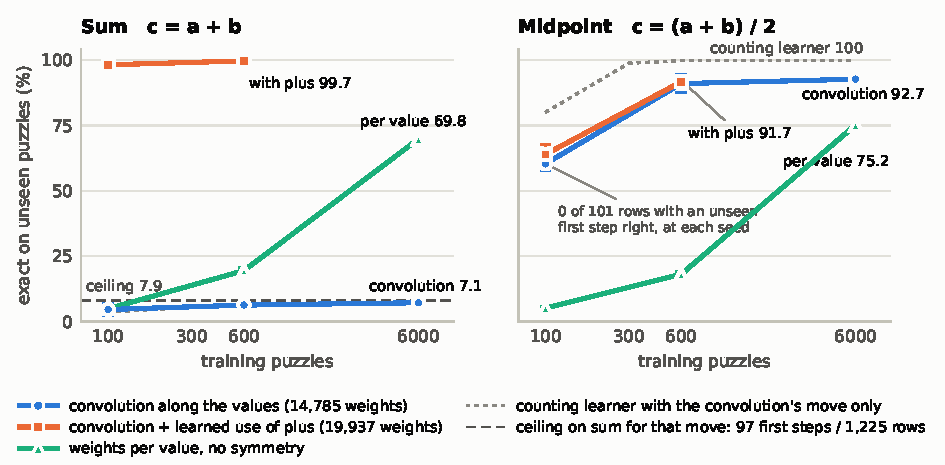
\includegraphics[width=\linewidth]{figures/twins_sum_midpoint}
\caption{Exact \% on sum and on midpoint against training puzzles, for the convolution along the values (the shift built in), the same model with learned use of \texttt{plus}, and weights per value. Means of three seeds at 100 and 600 puzzles, one run at 6,000. The dashed line is sum's ceiling under the shift, 7.9\%, counted before training; the dotted line is the counting learner with the shift.}\label{fig:twins_sum_midpoint}
\end{figure}

The single runs of the first table agree with these means to within 3 points. The same comparison as a two-by-two table, with the means at 100 / 600 puzzles:

\begin{center}\small
\begin{tabularx}{\linewidth}{@{}YYY@{}}
\toprule
 & the model has the shift & the model has no value symmetry \\
\midrule
the rule keeps the shift (midpoint) & 60.3 / 91.0 & 5.0 / 18.0 \\
the rule does not (sum) & 4.5 / 6.2, ceiling 7.9 & 4.8 / 19.4 \\
\bottomrule
\end{tabularx}
\end{center}

\textbf{Without the symmetry the twins are equally hard.} With weights per value, sum and midpoint are within 1.4 points of each other at 100 and 600 puzzles over three seeds, and within 6 points at 6,000, and both track the memorising learner. The facet model has no consistent winner: sum is ahead at 600 puzzles and midpoint at 6,000. Nothing separates the two rules for a model that cannot use the shift.

\textbf{With the shift built in they part completely.} The same 14,785 weights reach 91.0\% on midpoint and 6.2\% on sum from 600 puzzles, with standard deviations of 3.4 and 0.8 points. On midpoint the shared model at 600 puzzles is ahead of weights per value at 6,000 (75.2), with 3\% of the weights and a tenth of the data. Mirror behaves like midpoint, so the gain does not come from midpoint's answers lying between its operands.

\textbf{Sum stays at its ceiling.} 7.1\% at 6,000 puzzles against the 7.9\% computed in advance, and between 1.8\% and 7.1\% in each of the six seeded runs at 100 and 600 puzzles, at the epoch picked on the selection puzzles. The ceiling is on the expected accuracy, and the 507 unseen sum rows fix a 7.9\% rate only to about 1.2 points. Over all 172 evaluated epochs of these runs, 8 are above 7.9 and the highest is 9.7, in the run on 6,000 puzzles, whose epochs average 7.9. The model is at the ceiling, not measurably under it. That a model which reads the question row through a shift-equivariant kernel cannot fit a rule that does not keep the shift follows from the algebra of Section~\ref{sec:7.3} and is no discovery. It is a check that the symmetry is really built in, and it shows what a mismatched symmetry costs here: 63 points against weights per value at 6,000 puzzles, on a rule the model could otherwise learn.

\textbf{No symmetry is not what makes a rule hard.} Lookup has none, and weights per value learn it from 600 puzzles (97.5), because it has 51 rows. Sum is expensive for a model without the right symmetry because its table is large \emph{and} nothing collapses it. A large table with the right symmetry is cheap (midpoint, shared), and a small table needs none (lookup).

\section{What the network generalises is what its orbits allow}\label{sec:7.5}

The shared network reaches 60.3 / 91.0 / 92.7 on midpoint where the counting learner reaches 80.0 / 99.8 / 100. Part of the distance has a plain cause: the counting learner is told which rule a row follows, and the network is not. A midpoint row whose first step is ±2 looks, from the question row alone, like a Progression row. At 6,000 puzzles the network gets none of those 33 rows right and 469 of the other 472.

The more telling comparison is on rows whose first step never occurred in a training question. The checkpoints are those of the seeded table in Section~\ref{sec:7.4}, seeds 1 / 2 / 3.

\begin{center}\small
\begin{tabular}{@{}lll@{}}
\toprule
shared model, midpoint & first step seen in training & first step never seen \\
\midrule
100 training puzzles & 71.5 / 77.5 / 77.2\% of 404 rows & \textbf{0 / 0 / 0} of 101 rows \\
600 & 87.3 / 93.3 / 93.1\% of 504 & 0 / 0 / 0 of 1 \\
\bottomrule
\end{tabular}
\end{center}

Not one row with an unseen first step is answered correctly, at either size or any seed. This is what the model's parameterisation implies. The answer is linear in the first step, c = b − (b − a)/2, but the kernel has one free weight vector per offset and nothing ties the vectors of two offsets together, so the template has no way to carry ``half the step back'' from the steps it has seen to one it has not (Statement 11 holds for it nearly as it stands). The model fills the orbits the convolution gives it, one at a time, as the counting learner does, only less efficiently. Weights per value do the same one level down: at 100 puzzles they get 20 to 24 of the 25 rows whose pair (a, b) they have seen and 3 or 4 of the other 480. In both models, what generalises is exactly what the built-in symmetry merges. The result is not a finding about neural networks in general, which with a smooth kernel or numbers as inputs could do otherwise. Its use is that the count says, before training, which rows a model of this family will get.

How many training rows an orbit needs can be read from the same checkpoints. Pooled over the three seeds, an unseen row with exactly one training question in its orbit is answered correctly in 422 of 573 cases at 100 puzzles (74\%) and in 71 of 72 at 600 (99\%). With three or four training questions it is 92\% at 100 puzzles. One row per orbit is thus enough once the rest of the network has been trained, which is what the count assumes. The pairs that weights per value get right without having seen them, 11 of 1,440 over the three seeds, are the rate of guessing among 101 values.

\section{The reversal: giving the model the relation sum needs}\label{sec:7.6}

If the argument is right, sum should become as cheap as midpoint in a model that has sum's own moves. The move ``one operand and the answer together'' is what a relation \texttt{plus(U, W, V)} for U + W = V expresses when it is supplied as background facts: (u + s) + w = v + s. We added these facts to the shared model, with learned rules that walk through them (Section~\ref{sec:4.5}), and removed nothing else. The model has 19,937 weights. \emph{Prediction from the counting learner:} with sum's moves, sum is learned from the first few puzzles; midpoint keeps what the convolution gives it.

\begin{center}\small
\begin{tabularx}{\linewidth}{@{}YYY@{}}
\toprule
shared model, three seeds & sum, 100 / 600 puzzles & midpoint, 100 / 600 puzzles \\
\midrule
without \texttt{plus} & 4.5 ± 2.3 / 6.2 ± 0.8 & 60.3 ± 2.7 / 91.0 ± 3.4 \\
with \texttt{plus} used by learned rules & \textbf{98.2 ± 0.8 / 99.7 ± 0.4} & 63.9 ± 3.9 / 91.7 ± 1.8 \\
\bottomrule
\end{tabularx}
\end{center}

The model that was held under 8\% learns sum from 100 puzzles. Midpoint is where it was: the differences of 3.6 and 0.7 points are inside the spread of the seeds, so the added facts neither help nor hurt it.

How much this gives away has to be said plainly. A function that respects every one of sum's moves is a + b + k for a single number k. Sum's full group of moves is thus the rule itself up to one constant, and the counting learner with these moves has a single orbit and is right after ten puzzles. The convolution gave midpoint one of the two directions of its group, which left 50 orbits to learn; \texttt{plus} gives sum everything, which leaves one. That is why 98.2 is above 60.3, and it does not mean sum is the easier rule. \texttt{plus} is the relation handed over as background knowledge. What the network learns is when to use it and how to read the result. Learning sum then becomes choosing and reading a given relation, much as in models with programmed rules, PrAE (\citealp{zhang2021abstract}) and ARLC (\citealp{camposampiero2024towards}). The section measures the price of that knowledge, not a way of learning arithmetic. It also has a cost in size: there is one \texttt{plus} fact per pair of values, so their number grows with the square of the value range, and the value axis was not run on I-RAVEN-X's range of 1,000. The general statement is this: the more of a rule's group is built in, the fewer orbits are left to learn, and at one orbit the rule has been given.

The same switch on the benchmark's own Arithmetic, in puzzles where the four rules are mixed:

\begin{center}\small
\begin{tabularx}{\linewidth}{@{}YlY@{}}
\toprule
value axis, Arithmetic exact & without \texttt{plus} & with \texttt{plus} in learned rules \\
\midrule
I-RAVEN-X, rows of 3, values 0–10 & 70.7 & 98.8 \\
I-RAVEN-X, rows of 10, values 0–50 & 11.1 & 100 (88.7 when other moves along the values compete) \\
\bottomrule
\end{tabularx}
\end{center}

Without \texttt{plus} the other three rules stay at 100\% exact on rows of 10 and Arithmetic falls to 11.1\%. These rows are value-axis models compared with one another. The models of Chapter~\ref{ch:5}, which have to learn sums from codes, are in the right-hand column of the two-by-two table: they have no symmetry on the values, and for them a large table is simply expensive.

\section{A second symmetry: scaling}\label{sec:7.7}

Section~\ref{sec:7.5} ended on a claim that can be tested: what generalises is what the built-in symmetry merges. If that is right, a model with a second symmetry of midpoint must answer rows with unseen first steps, in the orbits the new symmetry merges and in no others. Midpoint has such a symmetry. Multiply every value by the same number k and the row stays valid: ka + kb = 2kc. In the terms of Section~\ref{sec:2.4}, the shift makes the zero of the value scale a convention, and scaling makes its unit a convention too: together they are Stevens's interval scale, except that on the ring a scaling may also be negative, which his interval scale, being ordered, excludes.

\textbf{The model.} The shared model's kernel has one weight per offset between two values. The new kernel counts offsets in each row's own unit: a value V lies k units from a value U, V = U + k·S, with one weight per k. The unit S is a constant like the values, and the template never names it. Background facts say which step is k units of S on the model's ring of 101 values. Since 101 is prime, every step has every multiple and every fraction on the ring, half a step included. A rule derives a row's unit from its first two panels, in one of two ways.

\begin{itemize}
\item \textbf{Doubled.} The unit is the largest power of two in the row's first step. The model is equivariant to doubling all values, and first steps that differ by a power of two fall into one orbit: 26 orbits in place of 50.
\item \textbf{Scaled.} The unit is the first step itself. The model is equivariant to v → kv + s for every k and s, and all first steps are one orbit. It can only answer c = b + g·(b − a) for a number g it has to learn. For midpoint g is −1/2. As \texttt{plus} does for sum (Section~\ref{sec:7.6}), this hands over the rule up to one number.
\end{itemize}

Both have the shared model's 14,785 weights. With random weights, the output of a transformed puzzle equals the transformed output to 2·10⁻¹⁷ on 100 puzzles, for every k and s in the scaled model and for doubling in the doubled one wherever the doubled steps stay in range. These are exact on the ring; on the values 0 to 50 a scaling sends most rows out of range, and Section~\ref{sec:3.7.1} says what that leaves. The shared model has neither symmetry (a difference of 2·10⁻²).

\textbf{Predictions, made before training.} At 100 training puzzles, 101 of the 505 unseen midpoint rows have a first step that no training question had. For 72 of them a training question had the same odd part of the step, for 29 none had.

\begin{center}\small
\begin{tabularx}{\linewidth}{@{}YYll@{}}
\toprule
 & shared & doubled & scaled \\
\midrule
orbits of first steps, midpoint & 50 & 26 & 1 \\
the 72 rows: new first step, odd part seen & none right (measured) & can be right & can be right \\
the 29 rows: new first step, new odd part & none right (measured) & none right & can be right \\
ceiling on sum & 7.9\% & 7.2\% & 1.4\% \\
\bottomrule
\end{tabularx}
\end{center}

\textbf{Results.} Exact \% on the tested rule, three seeds, the selection rule of Section~\ref{sec:7.4}.

\begin{center}\small
\begin{tabular}{@{}llll@{}}
\toprule
 & shared & doubled & scaled, seeds 1 / 2 / 3 \\
\midrule
midpoint, 100 puzzles & 60.3 ± 2.7 & 49.9 ± 5.3 & 19.0 / \textbf{100.0} / 21.0 \\
midpoint, 600 & 91.0 ± 3.4 & 67.5 ± 2.0 & 29.5 / \textbf{100.0} / 20.2 \\
sum, 100 & 4.5 ± 2.3 & 3.6 ± 0.2 & 3.2 / 0.8 / 2.0 \\
sum, 600 & 6.2 ± 0.8 & 4.1 ± 0.3 & 3.4 / 1.0 / 3.4 \\
\bottomrule
\end{tabular}
\end{center}

\begin{center}\small
\begin{tabularx}{\linewidth}{@{}Ylll@{}}
\toprule
unseen midpoint rows right at 100 puzzles, seeds 1 / 2 / 3 & shared & doubled & scaled \\
\midrule
the 72 rows & 0 / 0 / 0 & \textbf{50 / 43 / 39} & 18 / 72 / 19 \\
the 29 rows & 0 / 0 / 0 & \textbf{0 / 0 / 0} & 4 / 29 / 4 \\
\bottomrule
\end{tabularx}
\end{center}

The line the count drew holds at every seed. The doubled model answers more than half of the 72 rows on which the shared model answers none, and none of the 29. The scaled model has no group at zero; at one seed it answers all 101, and every other row, from 100 puzzles.

\textbf{What the count left out.} The totals fell, and the scaled model failed at two seeds of three. The cause is the confusion of Section~\ref{sec:7.5}, enlarged. The benchmark's Progression steps by 1 or 2. In a model that reads rows in a unit, a midpoint row whose first step is one unit begins exactly like a Progression row, and the network continues it as one: it generates 2b − a. At 600 puzzles, seeds 1 / 2 / 3:

\begin{center}\small
\begin{tabularx}{\linewidth}{@{}lYYY@{}}
\toprule
model & midpoint rows that begin like a Progression row & right among them & right among the other rows \\
\midrule
shared & 33 of 505 (first step ±2) & 0 / 0 / 0 & 440 / 470 / 469 of 472 \\
doubled & 152 (first step a power of two) & 1 / 11 / 1 & 330 / 340 / 340 of 353 \\
scaled & 505 (every row) & 149 / \textbf{505} / 102 & none \\
\bottomrule
\end{tabularx}
\end{center}

In the scaled model a midpoint question row and a Progression question row are the same picture, two panels one unit apart. Only the two complete rows above tell the rules apart. At one seed the model uses them: it is then right on all 505 rows from 100 puzzles, from the twentieth epoch on. At the other two seeds it continues four rows in five as a Progression.

\textbf{Why two seeds fail.} Two explanations were tested on the saved runs. The first was the answer layer: it adds the rule descriptor to the kernel's features and cannot switch a feature off by the rule. A gate from the rule descriptor on those features (1,056 more weights, the symmetries unchanged) was predicted to bring the scaled model to 100\% at every seed and to repair the shared model's 33 rows. Both predictions failed: the gated scaled model reaches 20 to 30\% at all three seeds and both sizes, and the gated shared model is right on none of the 33 rows.

The second was measured directly. The model reads a complete row through a row descriptor: the features of each neighbouring pair of panels, summed over all values and averaged over the row. Asked for that descriptor on unseen puzzles, the saved networks give (largest difference per feature, on a scale of −1 to 1):

\begin{center}\small
\begin{tabularx}{\linewidth}{@{}YYY@{}}
\toprule
runs & midpoint & row descriptor: a midpoint row against a Progression row \\
\midrule
scaled, seed 2, 100 and 600 puzzles & 100.0, 100.0 & 1.5, 1.4 \\
scaled, seeds 1 and 3; scaled with the gate (10 runs) & 19.0 to 30.5 & below 0.0001 \\
shared, with and without the gate (12 runs) & none of the 33 rows & below 0.0001 \\
\bottomrule
\end{tabularx}
\end{center}

In the 22 runs that fail, the descriptor is one vector whatever the row: it does not carry the row's steps, so the rule never reaches the answer. In the two runs that succeed it separates the rules. The template allows this. Summed over every value of the ring, the pair's features contain each kernel weight once wherever the two panels lie, so the sum depends on their step only through the curvature of the tanh. Why training grows that part at one initialisation and not at the others was not measured.

What the failed runs use instead is a cue that sits in the rule descriptor directly: whether the question row shares a value with a complete row. At 600 puzzles they are right on 101 to 107 of the 108 midpoint rows with a shared value and on 0 to 47 of the 397 without.

\textbf{The repair.} If that is the cause, a row descriptor that carries the steps must remove both failures, the scaled model's two outcomes and the shared model's 33 rows. We let the descriptor read each neighbouring pair's step directly: the first panel's kernel feature at the second panel's value, which is the kernel weight of exactly that step, counted in the row's unit where rows are read in one. Nothing else changes. The model has 2,048 more weights and the same symmetries (4·10⁻¹⁷ with random weights). \emph{Predictions, written before the runs:} the scaled model reaches 100\% at every seed; the doubled model answers more than half of its 152 rows that begin like a Progression row; the shared model answers some of its 33; the descriptor separates the two rules in every run.

\begin{center}\small
\begin{tabularx}{\linewidth}{@{}YYY@{}}
\toprule
midpoint, exact \%, seeds 1 / 2 / 3 & 100 puzzles & 600 puzzles \\
\midrule
shared, the descriptor reads the steps & 54.9 / 63.4 / 61.4 & 96.0 / 99.4 / 99.4 \\
doubled, the descriptor reads the steps & 90.1 / 91.3 / 86.1 & 99.4 / 99.0 / 99.2 \\
scaled, the descriptor reads the steps & \textbf{100.0 / 100.0 / 100.0} & \textbf{100.0 / 100.0 / 100.0} \\
\bottomrule
\end{tabularx}
\end{center}

All four hold. The scaled model is right on all 505 rows in each of its six runs, from the first evaluated epoch on. The shared model answers its 33 rows at every seed at 600 puzzles, and 17 to 27 of them at 100; in twelve runs without the repair it had answered none. The doubled model answers 151 or 152 of its 152 at 600 puzzles and 147 to 152 at 100. In all 18 runs the descriptor of a midpoint row differs from that of a Progression row by 0.9 to 2.0. The line the count drew among the unseen first steps holds as before: at 100 puzzles the doubled model answers 64 to 69 of the 72 rows it may and none of the 29 it may not, and the scaled model all 101. One further prediction was missed by one row: the shared model was to stay at none of the 101 and is right on one, at one seed, which is the rate of guessing among 101 values.

Sum stays capped, as counted. The doubled model gets 3.6 and 4.1\% against a ceiling of 7.2. The scaled model gets at most 3.4\%: at two seeds it continues every sum row by its first step and is right on exactly the 17 unseen rows with b = 2a, which is the most that one multiple reaches on these rows.

\textbf{What this adds.} First, the claim of Section~\ref{sec:7.5} survived a test it could have failed: the rows that became answerable are the ones the count named, and the rows it excluded stayed at zero. Second, a symmetry acts on all the data at once. Scaling is a symmetry of every rule here, but the generator never scales a Progression, so the size of the first step told the rules apart, and the shared model was using it. The symmetry removed that cue together with the differences it was meant to remove. This is the gap of Section~\ref{sec:6.5} seen from the other side: there a symmetry closed a shortcut that hurt on transformed puzzles, here it closed one that helped on the benchmark's own. A count over one rule's table cannot see this; a count over the question rows of all rules would. Third, the scaling model that succeeds learns one number, so its 100\% is the rule given, not the rule found. Fourth, the lost accuracy was not the price of the symmetry. With the cue gone, the model has to read the rule from the complete rows, and the first row descriptor did not carry it in 22 runs of 24. The shared model had the same defect and met it on 33 rows of 505; the scaled model met it on every row. With a descriptor that reads the steps, more of the rule's symmetry means less data at every step: 59.9, 89.2 and 100.0\% from 100 puzzles for the shift, doubling and scaling.

\textbf{Limits.} Three seeds, 200 epochs and no tuning. The ladder as printed is the second attempt: the first descriptor failed, the cause was measured, and the repair was predicted before it was run. Why the pooled descriptor loses the steps in training was not studied; with random weights it still separates the two rules a little. On sum the models with the repaired descriptor stay at their ceilings, as predicted before the runs: 4.0 and 7.6, 3.4 and 5.2, 1.2 and 1.6 at 100 and 600 puzzles against 7.9, 7.2 and 1.4. The repair was to the descriptor, and on sum the limit is where the answer is read: from the question row only. The doubled model's runs without the repair were not probed. Scaling is exact on the ring of 101 values, not on the range 0 to 50.

\section{A ladder of priors, and values read as numbers}\label{sec:7.8}

Sections~\ref{sec:7.6} and \ref{sec:7.7} ended on the same remark: the more of a rule's group is built in, the fewer orbits are left to learn, and at one orbit the rule has been given. This section puts the models of the chapter in that order and adds the one that is missing at the top.

\textbf{The top of the ladder.} Every model so far treats a value as a symbol (Section~\ref{sec:7.2}). Read the values as numbers instead, and assume the form c = pa + qb. Then nothing has to be learned from other puzzles: the two complete rows of a puzzle are two equations for p and q. We fit them by least squares for each attribute and apply them to the question row. The fit is not told which rule an attribute follows. \emph{Prediction:} it solves every rule of this form and no other.

\begin{center}\small
\begin{tabularx}{\linewidth}{@{}Yllll@{}}
\toprule
exact \%, unseen puzzles, no training & the tested rule & Progression & Constant & Distribute Three \\
\midrule
sum puzzles & 99.6 & 98.7 & 100 & 0 \\
midpoint puzzles & 99.8 & 99.3 & 100 & 0 \\
mirror puzzles & 99.8 & 98.7 & 100 & 0 \\
lookup puzzles & 1.7 & 98.6 & 100 & 0 \\
\bottomrule
\end{tabularx}
\end{center}

It does. Sum, midpoint and mirror are solved without one training puzzle, and so are Progression and Constant, which have the same form. On the sum, midpoint and mirror puzzles, each of its 32 misses on these rules is a puzzle whose two complete rows do not determine p and q. On lookup and Distribute Three, which are not linear, it gets 1.7\% and nothing.

\textbf{The ladder.} Midpoint at 100 training puzzles, in the order of how much is built in. The counting learner keeps one answer per orbit and is told the rule (Section~\ref{sec:7.3}).

\begin{center}\small
\begin{tabularx}{\linewidth}{@{}YYlY@{}}
\toprule
built in & left to learn & counting learner & trained model \\
\midrule
nothing about the values (weights per value) & 1,250 rows & 5.0 & 5.0 ± 0.5 \\
the shift: only differences count & 50 orbits & 80.0 & 59.9 ± 4.5 \\
the shift and doubling & 26 orbits & 94.3 & 89.2 ± 2.7 \\
the shift and scaling: only ratios of differences count & 1 orbit, one number & 100 & 100.0 / 100.0 / 100.0 \\
the linear form, values as numbers & nothing from other puzzles & – & 99.8 with no training \\
\bottomrule
\end{tabularx}
\end{center}

The three rows with a symmetry are the models whose row descriptor reads the steps (Section~\ref{sec:7.7}). With the first descriptor they reached 60.3 ± 2.7, 49.9 ± 5.3 and 19.0 / 100.0 / 21.0. At 600 puzzles the same four models reach 18.0, 98.3, 99.2 and 100.0.

The same for sum:

\begin{center}\small
\begin{tabularx}{\linewidth}{@{}YYlY@{}}
\toprule
built in & left to learn & counting learner & trained model \\
\midrule
nothing about the values (weights per value) & 1,225 rows & 4.7 & 4.8 ± 0.6 \\
the shift, with the answer read from the question row & a ceiling of 7.9\% & 3.6 & 4.5 ± 2.3 \\
addition's own moves (\texttt{plus}) & 1 orbit, one number & 100 & 98.2 ± 0.8 \\
the linear form, values as numbers & nothing from other puzzles & – & 99.6 with no training \\
\bottomrule
\end{tabularx}
\end{center}

\textbf{What the ladder says.}

\begin{itemize}
\item \textbf{Each rung is a piece of knowledge about numbers.} That values lie on a line (the shift), that the line has no fixed unit (scaling), that values can be added (\texttt{plus}), that the rule is linear. Each has a price in training puzzles, and the count gives that price before training.
\item \textbf{The trained models end in the count's order, at the second attempt.} The count says every rung needs less data than the one below it, and from 100 puzzles the networks reach 5.0, 59.9, 89.2 and 100.0\%. They stay under the count where many orbits are left: by 20 points with the shift, by 5 with doubling, by nothing with scaling. The order held only once the model could read the rule from the complete rows. With the first row descriptor the two scaling rungs fell below the rung beneath them (Section~\ref{sec:7.7}), with the same groups and the same counts. The count bounds what a model of this family can reach and orders the rungs; how close a network comes depends also on how it describes a row, and the 20 points with the shift alone are not explained.
\item \textbf{A prior and the answer are two ends of one scale.} At the top nothing is left to learn across puzzles, and at one orbit a single number is. What is left to learn, counted in orbits, is a unit on that scale. \citet[pp. 1 and 43]{chollet2019measure} asks that skill be reported together with the priors and the experience behind it (Section~\ref{sec:2.4}). For one rule and one family of models, the amount of prior can here be counted.
\item \textbf{The top rung has its price too.} The linear form gives nothing on Distribute Three and on lookup, as the shift gives nothing on sum. The worth of a prior belongs to the pair of model and rule at every rung.
\end{itemize}

Which rung a model should start from is not something the count decides. Models in which addition is an operation of the representation start from the upper rungs (Section~\ref{sec:2.5}). A template that treats values as constants starts at the bottom, and this chapter measured what each step up costs it.

\section{What the experiment shows, and its limits}\label{sec:7.9}

\textbf{What it shows.} A symmetry prior is not good or bad in itself. The same convolution is worth an order of magnitude of data on midpoint and costs nearly everything on sum. Its worth belongs to the pair of model and rule, and for this pair it was computed before training: 50 orbits in place of 1,250 rows on one side, a ceiling of 7.9\% on the other. The trained networks sat at the ceiling, came close to the saving (59.9\% against the count's 74.8\% at 100 puzzles, 91.0\% against 98.7\% at 600, and 98.3\% once the row descriptor read the steps), and, as their weights per offset imply, got no row the count did not allow. Section~\ref{sec:7.8} puts the same statement on one scale: from weights per value to the linear form, each piece of built-in knowledge leaves less to learn, down to nothing.

\textbf{Objections.}

\begin{itemize}
\item \emph{``Read the values as numbers and both rules are trivial.''} They are: a linear fit on a puzzle's two complete rows solves them with no training (Section~\ref{sec:7.8}). That model is given the form of the rule. The twins test what a model pays that is not given it, which is the position of every template in this thesis, and of any model on a rule that is not linear, where the numbers do not help.
\item \emph{``A shift-equivariant model cannot fit a rule that is not shift-equivariant. That is obvious.''} For a model that answers from the question row it is, and Section~\ref{sec:7.4} says so. What is not obvious is that the two rules are otherwise equally hard, and that the size of the gain on midpoint, and which rows it covers, are given by a count.
\item \emph{``Your model sees the complete rows, and from them a shift-equivariant function can compute a sum.''} It can (Section~\ref{sec:7.3}). The ceiling holds for this template because it never measures from one row to another, and Section~\ref{sec:7.3} says that this is a property of the template and not of the shift.
\item \emph{``Midpoint is not a rule of the benchmark.''} It is a probe, built to isolate one property. The evidence on the benchmark is Section~\ref{sec:7.6} and the value-shift ablation of Section~\ref{sec:6.2}.
\item \emph{``These are not groups on the values 0 to 50.''} Correct. A shift can leave the range, midpoint needs a + b even, and the shared model's ring wraps around where the data does not. The orbit counts were made on the actual tables, so the numbers stand; the group language is exact only away from the ends of the range.
\end{itemize}

\textbf{Limits.}

\begin{itemize}
\item \emph{The test range came last.} Every checkpoint of this chapter was scored once on puzzles 8000 to 9999 at the end of the work, with 963 midpoint and 1,014 sum rows (Appendix~\ref{sec:D.6}). The seeded cells move by at most 3.2 points, each within the sampling error of the 500 rows reported here. Every sum mean stays at or under its ceiling within sampling error, and the ladder keeps its order: with the steps at 100 puzzles, 59.4, 88.2 and 100 against the counts 80.0, 94.3 and 100. The facet model on sum at 600 puzzles moves the most, from 31.2 to 24.7, so its lead over midpoint there shrinks from 7 points to 3. The cells at 6,000 puzzles of the shared and per-value models cannot be tested as reported, because their runs saved another epoch than the one the table reads.
\item Sum and midpoint at 100 and 600 puzzles have three seeds, with standard deviations up to 3.9 points. Three runs fix a standard deviation only to about half its size. The cells at 6,000 puzzles, mirror, lookup and the facet model are one run of about 500 rows, so ±4 points. The effects reported are 50 points and more; differences of a few points between cells mean nothing.
\item The epoch is picked by exact score on the selection puzzles here, because matched is near 100\% for every model on these puzzles and picks arbitrary epochs. The conclusion is the same under either choice. For sum in the shared model the choice is arbitrary under either: the whole-puzzle score does not move with a rule the model cannot learn, and one seed's cell at 100 puzzles (1.8\%) is such an epoch.
\item The runs at 6,000 puzzles with weights per value and the facet model were still improving when they stopped. The comparisons at 100 and 600 puzzles are the firm ones.
\item The experiment is on rows of 3. That Arithmetic on rows of 10 is hard for the models of Chapter~\ref{ch:5} for the same reason is an inference: their table there has billions of rows and they have no symmetry that collapses it.
\item Every trained model here treats values as symbols (Section~\ref{sec:7.2}). The comparison between sum and midpoint is a statement about such models; with values as numbers and the linear form given, neither rule needs training.
\item The ladder of Section~\ref{sec:7.8} has three seeds per rung, and its three rungs with a symmetry use the row descriptor that was repaired after the first one failed. It is a second attempt, with the repair predicted before it was run. The first attempt shows that, for one group and one orbit count, the way a model describes a row can decide between 20\% and 100\%. The count predicts the order and the reach of the rungs, not the accuracy of a given network.
\end{itemize}

\chapter{Discussion and conclusion}\label{ch:8}

\section{What a symmetry is worth}\label{sec:8.1}

The thesis asked what a built-in symmetry is worth to a relational model, and whether that can be known before training. The answer the experiments give is a count with two sides and a condition.

Where the rule gives corresponding answers on the inputs a symmetry merges, the symmetry is worth the data it lets the model reuse. Where it does not, it is worth a ceiling. Both are numbers of orbits on the rule's table, and both were written down before the runs. The saving matters most in practice, because it is largest exactly where data is scarce and fades as data grows: tens of points at 100 to 600 training puzzles, a few at 6,000 (Section~\ref{sec:6.2}). Counted in puzzles rather than points, it is the size of the group the data really has. For the attributes that is two to three, not the three of the group the model was given, because type never carries Arithmetic; the runs needed that much data. The ceiling showed up twice: a reflection held a model near half of all values (Section~\ref{sec:6.7}), and the shift held one at 7\% on sums against the 7.9\% counted (Section~\ref{sec:7.4}).

The condition is on the learner. The count describes a learner that shares nothing across orbits and can tell every orbit apart. Our value models share nothing across orbits by construction, so they got the rows the count allows and none of the others (Section~\ref{sec:7.5}); that part follows from their weights. Whether a network also tells the orbits apart depends on how it reads the puzzle. With the first row descriptor the same group and the same count gave 20\% or 100\% (Section~\ref{sec:7.7}), and with the shift alone the network stays 20 points under the count at 100 puzzles, for a reason we did not find. The ceiling has a condition of the same kind: it belongs to the shift together with reading the answer from the question row, not to the shift alone (Section~\ref{sec:3.6.3}). The count bounds what a model of a given family can reach and orders the models by the data they need. It does not by itself give a network's accuracy.

So the answer to the second half of the question is yes, to the extent that the rule's table is known and the way the model reads the puzzle is part of what is counted. For a generated benchmark both are known. For a task where they are not, the count still says what to look for: the worth of a symmetry prior is a property of the pair of model and task, and a prior that helps on one rule can cap the model on its neighbour.

\section{Which symmetry, not how much}\label{sec:8.2}

It is tempting to summarise Chapter~\ref{ch:7} as ``Arithmetic is hard because it has no symmetry''. That is false, and the difference matters. Sum has as many moves that keep its rows valid as midpoint has. What it lacks is one particular move, the common shift, and that happens to be the move a convolution along the values builds in. Given its own moves, sum is the easier rule of the two.

The practical reading is that ``more equivariance'' is not a direction in which models improve. The convolution is the natural symmetry to put on a line of values, three of the benchmark's four rules have it, and on the fourth it turns a model that would have learned slowly into one that cannot learn at all. A designer who adds a symmetry is betting that every rule in the task shares it. The bet can be checked beforehand, by transforming valid examples and asking whether they stay valid and whether the answer moves with them (Section~\ref{sec:3.5}), and the stakes can be counted.

The same holds in the other direction. Midpoint keeps the shift and also scaling, and a model given both needs less data at every step: from 59.9\% with the shift alone to 100\% with scaling at 100 puzzles, once its row descriptor could read the steps of the complete rows (Sections~\ref{sec:7.7} and \ref{sec:7.8}). More of a rule's own symmetry helps; a symmetry the rule lacks caps.

\section{Sharing and invariance are two things}\label{sec:8.3}

Building a symmetry in gives a model two properties at once: its weights are shared across the things the symmetry exchanges, and its output is exactly invariant. The label experiments separate them. A model that shares its weights and is not invariant learns as fast as the invariant model on puzzles like the training ones (Section~\ref{sec:6.3}). It fails where the training data stops: on a rule never seen on an attribute it loses 44 points where the invariant model loses 5 (Section~\ref{sec:6.4}), and where the generator leaves room, it learns the generator's regularity in place of the rule (Section~\ref{sec:6.5}). A symmetry in that room can also pay on the benchmark itself: the order of Arithmetic's operands, which the generator never varies, adds 7 points at 6,000 puzzles and doubles the exact sums (Section~\ref{sec:6.6}).

Sharing, then, is what saves data, and invariance is what carries the model beyond its data. For a benchmark score only the first is needed, which is one reason a benchmark score says little about the second.

\section{Where the priors came from}\label{sec:8.4}

Every prior in this thesis was chosen by someone who had read the generator. The first objection to all of the above is therefore that the answer key was copied into the model. \citet{chollet2019measure} gives the terms for an honest reply. Skill can be bought with priors, and ``unlimited priors allow system developers to 'buy' unbounded performance on any given task'' (p. 25). A fair test may assume a short list of them, including objects, elementary geometry, and numbers, which ``may be added or subtracted'' (p. 26), with quantities ``smaller than approximately 10'' in his own benchmark (p. 49). And generating every task from one program is ``a weakness'', since reverse-engineering the program would solve them all (p. 51). RAVEN is generated from one program.

We sort our priors by whether a person would bring them to any test of this kind, or whether they are read off this generator.

\begin{center}\small
\begin{tabularx}{\linewidth}{@{}YYY@{}}
\toprule
prior & built in by & kind \\
\midrule
objects are units; their order means nothing & objects as nodes & general \\
the same rule holds in every row & rows 1 and 2 not named & general \\
any attribute can carry a rule & the attribute as a variable & general \\
only differences between values matter & the value axis & general \\
addition & \texttt{plus} facts & general for small numbers; beyond the list for values up to 50 \\
the two components of a layout behave alike & the component as a variable & generator \\
the list of attributes and their ranges & the input encoding & generator \\
the middle columns are operands & column roles & generator \\
rules run along rows, never columns & row facts in every model & generator \\
\bottomrule
\end{tabularx}
\end{center}

Read by kind, the prices are suggestive. The largest gains belong to general priors: the shift of values (61 points at 100 puzzles), addition (sum from 5\% to 98\%), and a graph with a node per attribute (86\% against 30\% at 300 puzzles, Section~\ref{sec:5.4}). The generator's priors bought less, and what they bought was gone at full data: 14 points for the components at 100 puzzles, none at 6,000. This is a comparison across different models and datasets, and we do not lean on it.

One generator prior is in every model here, ours and the baselines alike: that rules run along rows. Transposing an I-RAVEN matrix leaves 3\% of Progression instances valid (Section~\ref{sec:3.5}), so a model with rows as facts should fail on a transposed puzzle that a person would not notice had changed. It does. On transposed puzzles the facet model, the model with copy links and the row fold all fall from 95.8–97.4\% to 45.0–45.1\% matched, and to about 4\% exact. RAVEN's rules applied along rows keep 47.7\% of the same kind of puzzles, so the models fail as a perfect row-rule solver fails (Figure~\ref{fig:iraven_transposed} shows a transposed puzzle). This is the prior's cost away from the generator; its worth in training data was not measured. It limits what every score in this thesis means: accuracy on the generator's own distribution, bought partly with the generator's own structure. Nothing here is a claim about the tests people take.

\begin{figure}[tbp]
\centering
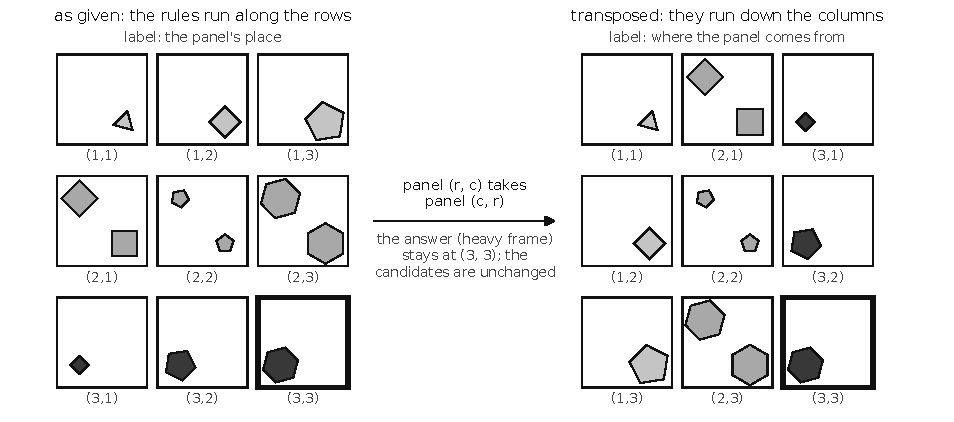
\includegraphics[width=\linewidth]{figures/iraven_transposed}
\caption{The I-RAVEN puzzle of Figure~\ref{fig:iraven_puzzle} as given and transposed: panel (r, c) takes the place of panel (c, r). The answer keeps its place (3, 3), so the candidates are unchanged, and the rules now run down the columns.}\label{fig:iraven_transposed}
\end{figure}

\section{What the lifted template contributes}\label{sec:8.5}

\textbf{Not accuracy.} A graph network in PyTorch with the same symmetries is within half a point of the facet model on I-RAVEN (Section~\ref{sec:5.5}). The gains reported in this thesis belong to the symmetries and to the graph.

\textbf{A uniform way to state and prove a symmetry.} In the template, a symmetry is the absence of a name. One theorem covers every case, and each was confirmed on random weights to machine precision. The baseline's symmetries were engineered into its node features one at a time, and each needed its own check. The ablations of Chapter~\ref{ch:6} are changes of a line in the template: add a fact that labels a component, or write a rule once per attribute. This is a difference in uniformity and convenience, not in what can be built: in a tensor framework, sharing weights over a set or a typed axis is also one line, and equivariant layers come with their own proofs.

\textbf{Relations of more than two things, used by learned rules.} \texttt{plus(U, W, V)} joins three values. In the template it is a fact like any other, and rules with weights walk through it (Section~\ref{sec:7.6}). A graph network that passes messages along pairs needs extra nodes for the triples to do the same, as networks on hypergraphs or factor graphs have; in the template no change of architecture is needed.

\textbf{Recursion.} The \texttt{plus} facts need not be given as a table. Two rules without weights derive them from the zero and the successor of each value, u + 0 = u and u + (w + 1) = (u + w) + 1, and the model's outputs are then identical to those with the table, to 2·10⁻¹⁶. The recursive rule is itself sum's symmetry: move one operand by one and the answer moves by one. All that a model needs to know about addition thus fits in a zero, a successor and one rule. It is written in and not learned, since weights cannot change which facts are derived, and it costs 22 times the grounding time on rows of 10.

\textbf{A cost.} Every puzzle becomes its own network, kept in memory, and trained one at a time on CPU: over 300 GB and about 15 hours for a run on all of I-RAVEN, where the PyTorch baselines need one GPU and a few gigabytes (Section~\ref{sec:5.8}). Background facts cost too: the \texttt{plus} facts grow with the square of the value range.

\section{Limits}\label{sec:8.6}

\begin{itemize}
\item \textbf{One seed.} Most numbers are a single training run. Where two seeds exist they differ by 1 to 2 points. Sum and midpoint at 100 and 600 puzzles have three, with standard deviations of 0.4 to 3.9 points for the models of Sections~\ref{sec:7.4} to \ref{sec:7.6}. So do Chapter~\ref{ch:6}'s comparisons with little data and the attributes at 6,000: standard deviations of 0.2 to 2.7 points, and each seed's gain within 2 points of the mean gain (+14.2, +13.5, +6.3). The vision transformer varies more: its gain from the exchange of rows is 8.6 to 28.0 points across three seeds. The first scaled model of Section~\ref{sec:7.7} had two outcomes, 100\% at one seed and about 20\% at two, which went with whether its row descriptor carried the rule; with a descriptor that reads the steps it is at 100\% in six runs of six. The conclusions rest on effects of 10 to 60 points and on their direction, not on differences of a point or two; the 0.4 points between the facet model and its PyTorch counterpart is not a result.
\item \textbf{The value axis is given the rules' primitives.} Its results are comparisons with itself. The symmetry on values, the centre of Chapters~\ref{ch:6} and \ref{ch:7}, has not been built into a model that learns the rules from codes. With \texttt{plus} given, learning sum is choosing a given relation, as in models with programmed rules, and the facts grow with the square of the range: the value axis was not run on values up to 1,000.
\item \textbf{One object per panel on I-RAVEN-X, and rows of 3 for the twins.} The orbit count was tested on tables of about 1,250 rows. That it explains the difficulty of Arithmetic on rows of 10 is an inference.
\item \textbf{The count needs the rule's table, and describes one kind of learner.} It was made on finite tables, where the groups hold only away from the ends of the range, and on a ring of 101 values where they hold exactly. It bounds a learner that shares nothing across orbits; how close a network comes depends on how it reads the puzzle (Section~\ref{sec:8.1}).
\item \textbf{Rows of 10 are not compared across model families.} The runs differ in training length and recipe (Section~\ref{sec:5.7}).
\item \textbf{Perception is trained apart}, with labelled objects, and the reasoning model cannot take graded inputs as it stands (Section~\ref{sec:5.3}). The pipeline is end to end at test time only, and its labels give it more supervision than the black-box transformer gets. A black-box reasoner given the same labels closes most of that gap only from 3,000 puzzles per layout (Section~\ref{sec:5.4}).
\item \textbf{The fixed encoding.} Thermometer codes tie the facet model to the value range it was trained on, and the list of attributes is given.
\item \textbf{The I-RAVEN-X test pass came last.} The text reports puzzles 6300 to 7299, which were looked at throughout the work. Every final checkpoint of Chapters~\ref{ch:5} to \ref{ch:7} was scored once on puzzles 8000 to 9999 only at the end, after an external review asked for it (Appendix~\ref{sec:D.6}). The test numbers agree with the reported ones within sampling error, except the facet model on sum at 600 puzzles, a single run, 24.7 against 31.2. Column roles' Arithmetic, the model chosen with the unseen puzzles in view, drops from 39.6 to 36.0, within sampling error but at every seed.
\item \textbf{One generator.} Section~\ref{sec:8.4}.
\end{itemize}

\section{Future work}\label{sec:8.7}

\begin{enumerate}
\item \textbf{Sum from differences, across rows.} A complete sum row shows where zero is, because c − b equals a. A function built from differences alone, c₃ = b₃ + (c₁ − b₁) + (a₃ − a₁), is right on every sum puzzle and follows a shift of the whole puzzle (Section~\ref{sec:7.3}). Our templates never measure from the question row to another row, which is why the shift caps them on sum. A kernel between a panel and the panel above it would give the model those offsets. The question is whether it then learns sum with the shift built in and without the \texttt{plus} facts. (The item that stood here, a row descriptor that reads each pair's step, was built and is Section~\ref{sec:7.7}'s repair: the scaled model then learns midpoint at every seed, so the cost measured there belonged to the descriptor and not to the symmetry. On sum it changes nothing, as predicted.) One caution: the function above chains two offsets, and a template that chains offsets for every answer contains it by construction. The test means something only if the chain is the same for every rule and the model still has to find which offsets to chain.
\item \textbf{Pricing ``rows only''.} The cost on transposed puzzles is measured (Section~\ref{sec:8.4}). What remains is its worth in data: replace rows by lines, with rows and columns both given as facts, so that the direction of a rule is inferred per attribute, and compare the two models at a few training sizes.
\item \textbf{Training perception and reasoning together.} The recognizer's output, the probability that a value exceeds each threshold, is already a soft thermometer code. The template has to lose its jump at zero first.
\item \textbf{The value axis on grids.} Position slots as constants with the geometry of the grid as background facts, and the number of objects as a line of its own, where Progression on positions is a cyclic shift.
\item \textbf{Learning the rule that derives addition.} The recursion of Section~\ref{sec:8.5} is written by hand. Finding it would be learning the structure of a template, not its weights.
\end{enumerate}

\section{Conclusion}\label{sec:8.8}

A built-in symmetry is worth the orbits it merges. Where the rule respects the symmetry, the model learns one answer per orbit and needs correspondingly less data; where it does not, the model is right on one input per orbit and no data helps. Both can be counted before training. In our experiments the trained networks sat at the counted ceiling, needed the counted amount of extra data where the models were otherwise equal, and came close to the counted saving once they could tell the orbits apart.

In a lifted relational template these symmetries are declared by leaving things unnamed, and hold exactly. A model built this way generates the answers of I-RAVEN without the rules and without the candidates: 97.2\% on the test split from object labels and 97.0\% end to end behind an object recognizer, against 93.1\% for a vision transformer with six times the weights, and 90\% against 16\% when each layout has 300 training puzzles, end to end as from labels. The recognizer learns from labelled objects and the transformer from the answer alone. Given the same labels, a black-box transformer over the recognizer's output gets 19\% from 300 puzzles per layout and needs about ten times the data to reach 90\%, so where data is scarce the gap is the structure, not the labels. A graph network with the same symmetries does as well, so the credit goes to the structure and not to the framework.

The assignment asked for symmetry-aware architectures that combine object recognition with priors on how objects compose, built on relational neural networks, and for an improvement over black-box vision. Chapters~\ref{ch:3} and \ref{ch:4} give the architectures and Section~\ref{sec:4.3} the recognition; Chapter~\ref{ch:5} gives the improvement, largest where data is scarce; and Chapters~\ref{ch:6} and \ref{ch:7} measure, prior by prior, what was bought and what a wrong choice would have cost.


\bibliographystyle{plainnat}
\bibliography{references}

\appendix
\chapter{PyNeuraLogic pitfalls}\label{app:A}

All PyNeuraLogic models in this thesis run on PyNeuraLogic 0.9.2, which executes on the Java virtual machine and on CPUs only. The five pitfalls below each cost real debugging time, and none of them produces an error message that points at its cause. Each is given with its symptom, its cause and the fix used in the code. A.6 lists the smaller ones.

\section{Isomorphic value compression must be off for native training}\label{sec:A.1}

\textbf{Symptom.} The symbolic templates, whose rules are given and only their weights learned (Section~\ref{sec:5.1}), trained badly: training accuracy collapsed, and the scores of some candidates did not move at all during training. Nothing was reported as wrong.

\textbf{Cause.} \texttt{Settings(iso\_value\_compression=True)}, the default, merges neurons whose \emph{initial values} coincide, as an optimisation for inference. In those models every weight starts at the same value, so the score of a candidate can start out equal to the value of a constant fact. The two neurons are then merged, and the candidate's score stays frozen at that constant for the whole of training. The optimisation is correct for a fixed network and wrong for one whose weights are about to change.

\textbf{Fix.} Every native training call in the code builds the model with

\begin{Verbatim}[fontsize=\small,breaklines]
model.build(Settings(optimizer=Adam(lr=args.lr), error_function=MSE(), iso_value_compression=False))
\end{Verbatim}

(\texttt{core/pynl/bench\_hub\_grounding.py}, \texttt{value\_axis.py}, \texttt{pynl\_symbolic.py}, \texttt{facet\_stream.py} and the scoring scripts). PyNeuraLogic's torch wrapper, \texttt{neuralogic.nn.torch\_function.NeuraLogic}, already switches it off, which is why the problem appears only in native training. The comment at the build call in \texttt{core/pynl/pynl\_symbolic.py} records how large the collapse was.

\section{Chain pruning removes the transformation of atoms with a single rule}\label{sec:A.2}

\textbf{Symptom.} A nonlinearity declared on an atom, such as \texttt{(R.rel / 3) | tanh}, has no effect. The network trains and its outputs look plausible, but part of it is linear where the template says it is not.

\textbf{Cause.} The default \texttt{chain\_pruning=True} removes every atom neuron of the grounded network that has a single incoming rule neuron, and its transformation goes with it. The query atom keeps its own. This acts on the ground network, not on the template text: an atom whose template has two rules, of which only one grounds for a given puzzle, loses its transformation as well. Aggregation does not protect an atom either: one rule averaged over several groundings still feeds the atom through one neuron. All three cases were checked on a toy template, where a tanh declared on a single-rule atom was applied with pruning off and dropped with it on, and kept in both settings once the same sum was split over two rules.

\textbf{Fix.} Turning chain pruning off is one option; on an early template it did not help (FINDINGS 9). The code keeps the default and splits the sum of an atom that needs its nonlinearity over two rules. In the facet template (Appendix~\ref{app:C}), \texttt{rel} and \texttt{ans}, and \texttt{relp} and \texttt{ansp} in the position channel, are written this way, which the code explains in a comment: without these two tanh layers everything after \texttt{vF} would be one linear map, which cannot express that the relation of the complete rows decides how the question row's panels combine. The copy gates and every step of the row fold are split in the same way so that their sigmoid and tanh survive. The other atoms with a single grounded rule keep the declared tanh only on paper: \texttt{f0}, \texttt{pv1}, \texttt{pv2}, \texttt{ctx}, \texttt{vP} and \texttt{ctxp}, and \texttt{vF} for the number attribute, whose second rule has no facets to ground on. Every result in this thesis was obtained with the template as printed in Appendix~\ref{app:C} and with this behaviour.

\section{Unweighted selector atoms add 1.0 unless declared hidden}\label{sec:A.3}

\textbf{Symptom.} The facet model, trained on all seven layouts, stayed far behind on the 2×2 and 3×3 grids, although its grid component is built exactly as in the in-out grid layout, where it did well. It placed the objects of every grid on one set of slots, and moving a puzzle's objects to other slots did not change the positions it generated.

\textbf{Cause.} In a lifted relational network an unweighted body atom contributes its value to the rule's sum. A ``selector'' atom that is meant only to ground the rule, such as \texttt{obj(P, O)} or \texttt{ocomp(O, C)} in the occupancy rule as it was written before the fix (printed with \texttt{--visible-selectors}),

\begin{Verbatim}[fontsize=\small,breaklines]
occ(P, C) :- obj(P, O), ocomp(O, C), pos(O). [transformation=identity, aggregation=sum]
\end{Verbatim}

has the value 1.0, so it adds 1.0 to every component of the result. Each object therefore added its one-hot slot \emph{plus 2 in every slot}, and the occupancy vector of a panel told the model little more than how many objects it held. This is the semantics of the formalism and not a defect of the library. The attribute channels suffered less, because they average over objects, so there the selectors add a constant instead of an offset that grows with the count.

\textbf{Fix.} Atoms that only ground a rule are declared hidden, \texttt{R.hidden.obj(...)}, printed with a leading \texttt{*} in Appendix~\ref{app:C}. \texttt{build\_facet\_template(..., hidden=True)} does this for every structural atom (\texttt{obj}, \texttt{ocomp}, \texttt{samepos}, \texttt{col}, \texttt{row}, \texttt{row3}, \texttt{full}, \texttt{qcomp}), and \texttt{--visible-selectors} restores the old behaviour as a control. Trained on the three grid layouts, the model went from 76.9\% to 92.4\% matched (FINDINGS 10). Hidden atoms are safe from version 0.9.2 on, which fixed a misalignment of weights around them. The weighted fact \texttt{puzzle(G)}, which serves as a bias, is unchanged.

\section{The Java runtime must be pinned on the compute nodes}\label{sec:A.4}

\textbf{Symptom.} A job that runs on the login node dies on an \texttt{amd} compute node with JPype's \texttt{JVMNotFoundException}, before any PyNeuraLogic code is reached.

\textbf{Cause.} \texttt{ml load Java/21} silently does nothing on the amd compute nodes of the cluster: \texttt{JAVA\_HOME} comes back empty, although the same module works on the login node. A second trap sits in the same place: a user site-packages folder for Python 3.11 shadows the conda environment with other versions of some libraries.

\textbf{Fix.} Every job script that runs PyNeuraLogic pins the runtime and switches the user site off:

\begin{Verbatim}[fontsize=\small,breaklines]
source /mnt/appl/software/Anaconda3/2024.02-1/etc/profile.d/conda.sh && conda activate pynl
export PYTHONNOUSERSITE=1 JAVA_HOME=/mnt/appl/software/Java/21.0.8 && export PATH=$JAVA_HOME/bin:$PATH
\end{Verbatim}

\section{Grounding memory}\label{sec:A.5}

\textbf{Symptom.} Large runs die while grounding, before the first epoch (an early run on I-RAVEN-X with rows of 10 and values 0–1000 died at 180 GB). A Jupyter kernel running PyNeuraLogic dies with the default heap of the virtual machine, and CPU-heavy kernels are killed on the login node anyway.

\textbf{Cause.} PyNeuraLogic grounds every puzzle into a network of its own and keeps all of them in the heap of the Java virtual machine. Memory therefore grows with the number of puzzles, with the length of the value codes and with the value range. Grounding takes 10–165 ms per puzzle, once (FINDINGS 13), but on the largest runs it took 30–45 minutes in all, and a grounded wide column-roles puzzle takes up to 12 MB. Updates are one puzzle at a time, since native training does not batch. By contrast, the torch baselines of the same size train on one GPU in a few GB.

\textbf{Fix.} The heap is set explicitly, \texttt{neuralogic.set\_max\_memory\_size(...)}, through \texttt{--jvm-gb} in \texttt{bench\_hub\_grounding.py}, and the job requests the memory that the run needs. The largest runs in RESULTS \S{}9 are:

\begin{center}\small
\begin{tabularx}{\linewidth}{@{}YYl@{}}
\toprule
run & memory requested / peak & time \\
\midrule
facet + copy links, I-RAVEN-X 3×10, values 0–1000 (5,426k weights) & 420 GB / 344 GB & 16.3 h \\
facet + content gates, I-RAVEN, all seven layouts & 420 GB / 327 GB & 15.0 h \\
row fold, 3×10, values 0–50 & 160 GB / 71 GB & 5.0 h \\
\bottomrule
\end{tabularx}
\end{center}

For the 100,000 Arithmetic-only puzzles of Appendix~\ref{app:E}, which do not fit a node, \texttt{core/pynl/facet\_stream.py} grounds the puzzles in chunks, again in every epoch. The rescoring job starts one process per checkpoint so that the virtual machine starts with an empty heap each time, and notebooks are executed as batch jobs on compute nodes.

\section{Smaller pitfalls}\label{sec:A.6}

The other pitfalls listed in FINDINGS 5, in brief:

\begin{itemize}
\item embedding tables must be declared as weighted facts, otherwise the rule silently fails to ground and the error names the query;
\item every sample needs its own query atom, because samples with the same query are merged without warning;
\item \texttt{build\_dataset()} may be called only once per built model;
\item \texttt{Aggregation.CONCAT} follows the grounder's order of the constants, not the order in which they were named;
\item rules with the same head are summed;
\item \texttt{Transformation.NORM} rescales any non-zero vector to unit length and leaves a zero vector at zero. In the facet model value 0 is the all-zero thermometer code, and since the template has no biases, a value of 1e-6 in its place flips outputs. This is why the facet model cannot take graded inputs from the recognizer without retraining (FINDINGS 39).
\end{itemize}

\chapter{Checks on the data}\label{app:B}

\section{The torch trainer reproduces the facet model's targets}\label{sec:B.1}

The torch baselines run in another environment (Python 3.7, torch, no PyNeuraLogic), so they cannot call the facet model's code. \texttt{data\_prep/prepare\_baseline\_data.py} therefore writes the facet model's puzzles and splits as plain arrays, and the baselines compute the targets and metrics from these arrays with their own code. To make sure that both compute the same thing, the same script also stores what the facet pipeline itself computes for the first puzzles of every split:

\begin{itemize}
\item \texttt{check\_target}: the facet model's target, \texttt{facet\_target}, for the answer panel of each of the first 20 puzzles, per component;
\item \texttt{check\_spec}: the decoded answer, \texttt{decode(describe(...))}, as one integer vector of occupancy bits and value counts per attribute.
\end{itemize}

Before training, \texttt{core/baselines/train\_baseline.py} recomputes both from the arrays for every split and stops unless the targets agree to 1e-6 and the decoded answers are identical. One exception is built in. I-RAVEN-X's Distribute rule draws values up to the maximum inclusive, one more than the codes and counts hold (FINDINGS 20). The code of that value stays distinct, so matching is unaffected, but the facet pipeline's decoder writes the value into the next attribute's counts. Such answers are left out of the decoded comparison, and the baselines score exact generation against the decoded true code. The facet model's own scorer had the same flaw: it capped exact generation at 95.6\% on 3×3 and at 98.4\% on 3×10. It was fixed and the I-RAVEN-X checkpoints were rescored on 2026-11-08; the facet model's 3×3 exact went from 92.7 to 97.0, and on 3×10 nothing moved by more than 0.6. Matching, the choice of epoch and the per-rule exact values were never affected.

The weights are checked in the same spirit. The baselines are sized to the facet model's weight count, which the script reads by building the facet template, and \texttt{train\_baseline.py} asserts that every model it builds has the number of weights it was sized to. All 102 torch checkpoints agree with their \texttt{best.json} (RESULTS \S{}9). For the test pass, \texttt{core/baselines/test\_eval.py} checks that the images and the label arrays list the same puzzles, and every checkpoint has to reproduce its recorded validation numbers exactly before it is scored on test once (RESULTS \S{}1).

\section{What the generators do to each rule}\label{sec:B.2}

Section~\ref{sec:3.5} gives, for each transformation of a puzzle, the share of rule instances that still satisfy a rule of the same kind afterwards, measured on 1000 training puzzles per I-RAVEN layout and 6000 per I-RAVEN-X file (\texttt{analysis/dataset\_symmetry\_check.py}). No instance fails its own label before the transformation. This section adds what the generators' code says about the same transformations, which explains the shares.

\begin{itemize}
\item \textbf{Rows 1 and 2 exchanged.} In the I-RAVEN generator each row starts from a fresh draw and is built by the same rule objects, and Distribute Three picks its direction with equal probability, so for rows of three the exchange maps one direction onto the other. The exchange is a data symmetry, with one small exception: for Arithmetic on colour the generator redraws row 2 so that plus and minus stay distinguishable. In I-RAVEN-X with rows of 10, Constant, Progression and Arithmetic rows are drawn independently, but a Distribute row is the first row rotated by a constant step. After the exchange no step fits. The exchanged puzzle is therefore never generated, yet its answer, the value that the third row lacks, stays the same: a symmetry of the task but not of the data. With rows of three the exchange survives, because a rotation by three steps leaves a row of three unchanged.
\item \textbf{Columns.} Progression dies under any exchange of columns, because a Progression row read in another order is not one. Constant survives every exchange, and Distribute survives an exchange of columns 1 and 2 in rows of three but not in rows of 10, where its rows are rotations. Of Arithmetic, what survives is the part that does not depend on the order of the operands: the plus rows under an exchange of columns 1 and 2, and every Arithmetic row of I-RAVEN-X under an exchange of middle columns. The generators do not draw the operands symmetrically, though. I-RAVEN draws the second operand from what the first leaves, and I-RAVEN-X draws its operands one after another from a shrinking range, shuffles them and then moves a zero out of the last operand slot. Most operands are zero, and the share of zeros depends on the column. Operand order is therefore a symmetry of the task but not of the data (Section~\ref{sec:6.6}).
\item \textbf{Values reflected}, v mapped to max − v. Constant and Distribute use only equality, and Progression uses order and the successor, so all three keep their rule. Arithmetic uses addition with zero and keeps nothing.
\item \textbf{Columns reversed}, which moves the missing panel. It maps a Progression step d to −d, plus to minus and one Distribute direction to the other, and it is a data symmetry of both generators on complete matrices. Because it moves the blank, it relates puzzles with different questions, so it is a symmetry for a model that fills any cell, not for ours. Union and difference on positions do not survive it: a union cannot be undone.
\item \textbf{Grid positions.} Progression on Position moves through the slots in reading order, cyclically, so only the grid maps that keep that cycle keep the rule: on the 2×2 grid the left-right and up-down mirrors and the half turn, on the 3×3 grid the half turn only. The set rules on positions (Constant, union and difference, Distribute) survive every permutation of the slots.
\item \textbf{Attributes.} In I-RAVEN-X, size and colour are drawn by the same function with the same rules and range, so exchanging them is an exact data symmetry. Type never carries Arithmetic (B.3), so exchanging type with size or colour holds only away from Arithmetic. I-RAVEN has no exact exchange of attributes: type, size and colour have 5, 6 and 10 values, Arithmetic on size has an extra +1, and type has no Arithmetic.
\item \textbf{Components.} The left and right components, and the upper and lower ones, have identical constraints and matching rule counts and means, so exchanging them is an exact data symmetry. The inner and outer components of the in-out layouts are not exchangeable: the outer object is always white and larger. Rules act on each component separately, so exchanging components is still a symmetry of the task in every layout.
\item \textbf{Nuisance.} \texttt{Angle} is drawn at random and no rule governs it (FINDINGS 3). The facts leave it out, so the models are invariant to it by construction.
\end{itemize}

\section{Rules per attribute in I-RAVEN-X}\label{sec:B.3}

On the I-RAVEN-X training puzzles 0–5999, size and colour each carry the four rules equally often, about 25\% each, while type never carries Arithmetic and carries each of the other three rules a third of the time (RESULTS \S{}7). A recount from the data file for rows of 10 and values 0–50, made for this appendix, agrees. Two consequences are used in the thesis. The attribute symmetry that the facet model builds in is exact between size and colour and holds for type only away from Arithmetic. And when weight sharing across attributes is priced in training puzzles (Section~\ref{sec:6.2}), the factor counted in advance is 2 on puzzles with Arithmetic, where only size and colour contribute examples, and between 2 and 3 overall; the runs met both counts.

\section{Other checks}\label{sec:B.4}

Three checks were made before any model was trained (FINDINGS 2 and 4, \texttt{analysis/sanity\_checks.py}, each with a negative control). I-RAVEN's annotation lists only the occupied slots of a grid, and deriving a slot from an object's index in that list, as the inherited code did, made about a third of the grid puzzles unanswerable; slots are now derived from the bounding boxes. No puzzle occurs in two splits, and the answer index is uniform. A model that sees only the eight candidates is at chance on I-RAVEN, against 90–100\% on RAVEN, and the annotation matches the images.

\chapter{The facet template}\label{app:C}

This is the facet template of Chapter~\ref{ch:4} as PyNeuraLogic prints it, in the configuration of the main I-RAVEN model (widths 32, 64 and 128; 10-bit codes; 22 slots; 266,528 weights). It was printed by building the template, without grounding or training:

\begin{Verbatim}[fontsize=\small,breaklines]
python3 -c "import sys; sys.path.insert(0, 'core/pynl'); import bench_hub_grounding as B; \
print(B.build_facet_template(32, 2, widths=[32, 64, 128]))"
\end{Verbatim}

\section{Notation}\label{sec:C.1}

\begin{itemize}
\item \texttt{h(X, Y) :- b1, b2.} is a rule with head \texttt{h} and body atoms \texttt{b1}, \texttt{b2}. Upper-case arguments are variables, lower-case ones are constants.
\item \texttt{\{m, n\} b(...)} multiplies the value of \texttt{b}, a vector of length n, by a learned m×n matrix. A body atom without braces enters with its own value, unweighted.
\item \texttt{*b(...)} marks a hidden atom: it takes part in grounding but adds nothing to the sum (Appendix~\ref{sec:A.3}).
\item \texttt{[aggregation=avg]} after a rule says how its groundings for one head are combined; \texttt{sum} is the other choice used here, and the library's default is the average. Rules with the same head are summed.
\item \texttt{h/2 [transformation=tanh]} sets the activation of every atom of predicate \texttt{h} with two arguments. Under the default chain pruning it is applied only where an atom has more than one grounded rule (Appendix~\ref{sec:A.2}).
\item \texttt{[combination=concat]} joins the body atoms into one vector instead of summing them; \texttt{elproduct} multiplies them element by element.
\end{itemize}

The facts of a puzzle are: \texttt{fv(O, A)}, the thermometer code of object O's value of attribute A; \texttt{nm(P, C)}, the code of the number of objects of component C in panel P; \texttt{pos(O)}, the one-hot slot of O; \texttt{obj(P, O)} and \texttt{ocomp(O, C)}, which place an object in its panel and component; \texttt{samepos(O1, O)}, for two objects in the same slot of two panels of one row; \texttt{col(P, c)}, the column of a panel; \texttt{row(Rw, P1, P2, P3)} and \texttt{full(Rw)} for the two complete rows; \texttt{row3(P1, P2)} for the two context panels of the question row; \texttt{qcomp(G, C)}, the component that the sample asks for; and \texttt{puzzle(G)}, a scalar fact of value 1. Panels are \texttt{p0} to \texttt{p7}, components \texttt{k0} and \texttt{k1}, and A ranges over \texttt{type}, \texttt{size}, \texttt{color} and \texttt{number}.

\section{The template}\label{sec:C.2}

\begin{Verbatim}[fontsize=\small,breaklines]
f0(O, A) :- {32, 10} fv(O, A).
f0/2 [transformation=tanh]
pv1(P, C, A) :- *obj(P, O), *ocomp(O, C), {64, 32} f0(O, A). [aggregation=avg]
f1(O, A) :- *obj(P, O), *ocomp(O, C), {64, 64} pv1(P, C, A).
f1(O, A) :- *samepos(O1, O), *obj(P, O), *col(P, c1), *obj(Q, O1), *col(Q, c2), {64, 32} f0(O1, A). [aggregation=avg]
f1(O, A) :- *samepos(O1, O), *obj(P, O), *col(P, c1), *obj(Q, O1), *col(Q, c3), {64, 32} f0(O1, A). [aggregation=avg]
f1(O, A) :- *samepos(O1, O), *obj(P, O), *col(P, c2), *obj(Q, O1), *col(Q, c1), {64, 32} f0(O1, A). [aggregation=avg]
f1(O, A) :- *samepos(O1, O), *obj(P, O), *col(P, c2), *obj(Q, O1), *col(Q, c3), {64, 32} f0(O1, A). [aggregation=avg]
f1(O, A) :- *samepos(O1, O), *obj(P, O), *col(P, c3), *obj(Q, O1), *col(Q, c1), {64, 32} f0(O1, A). [aggregation=avg]
f1(O, A) :- *samepos(O1, O), *obj(P, O), *col(P, c3), *obj(Q, O1), *col(Q, c2), {64, 32} f0(O1, A). [aggregation=avg]
pv1/3 [transformation=tanh]
f1(O, A) :- {64, 32} f0(O, A).
f1/2 [transformation=norm]
pv2(P, C, A) :- *obj(P, O), *ocomp(O, C), {128, 64} f1(O, A). [aggregation=avg]
f2(O, A) :- *obj(P, O), *ocomp(O, C), {128, 128} pv2(P, C, A).
f2(O, A) :- *samepos(O1, O), *obj(P, O), *col(P, c1), *obj(Q, O1), *col(Q, c2), {128, 64} f1(O1, A). [aggregation=avg]
f2(O, A) :- *samepos(O1, O), *obj(P, O), *col(P, c1), *obj(Q, O1), *col(Q, c3), {128, 64} f1(O1, A). [aggregation=avg]
f2(O, A) :- *samepos(O1, O), *obj(P, O), *col(P, c2), *obj(Q, O1), *col(Q, c1), {128, 64} f1(O1, A). [aggregation=avg]
f2(O, A) :- *samepos(O1, O), *obj(P, O), *col(P, c2), *obj(Q, O1), *col(Q, c3), {128, 64} f1(O1, A). [aggregation=avg]
f2(O, A) :- *samepos(O1, O), *obj(P, O), *col(P, c3), *obj(Q, O1), *col(Q, c1), {128, 64} f1(O1, A). [aggregation=avg]
f2(O, A) :- *samepos(O1, O), *obj(P, O), *col(P, c3), *obj(Q, O1), *col(Q, c2), {128, 64} f1(O1, A). [aggregation=avg]
pv2/3 [transformation=tanh]
f2(O, A) :- {128, 64} f1(O, A).
f2/2 [transformation=norm]
pt(P, C, A) :- *obj(P, O), *ocomp(O, C), fv(O, A). [transformation=identity, aggregation=avg]
pt(P, C, number) :- nm(P, C). [transformation=identity]
pt/3 [transformation=identity]
vF(P, C, A) :- {128, 10} pt(P, C, A).
vF(P, C, A) :- *obj(P, O), *ocomp(O, C), {128, 128} f2(O, A). [aggregation=avg]
vF/3 [transformation=tanh]
rel(Rw, C, A) :- *row(Rw, P1, P2, P3), {128, 128} vF(P1, C, A), {128, 128} vF(P2, C, A).
rel(Rw, C, A) :- *row(Rw, P1, P2, P3), {128, 128} vF(P3, C, A).
ctx(C, A) :- *full(Rw), {128, 128} rel(Rw, C, A). [aggregation=avg]
ans(C, A) :- *row3(P1, P2), {128, 128} vF(P1, C, A), {128, 128} vF(P2, C, A).
ans(C, A) :- {128, 128} ctx(C, A).
oa(G, A) :- {10, 1} puzzle(G), *qcomp(G, C), {10, 128} ans(C, A).
rel/3 [transformation=tanh]
ctx/2 [transformation=tanh]
ans/2 [transformation=tanh]
oa/2 [transformation=identity]
occ(P, C) :- *obj(P, O), *ocomp(O, C), pos(O). [transformation=identity, aggregation=sum]
occ/2 [transformation=identity]
vP(P, C) :- {32, 22} occ(P, C).
vP/2 [transformation=tanh]
relp(Rw, C) :- *row(Rw, P1, P2, P3), {64, 32} vP(P1, C), {64, 32} vP(P2, C).
relp(Rw, C) :- *row(Rw, P1, P2, P3), {64, 32} vP(P3, C).
relp/2 [transformation=tanh]
ctxp(C) :- *full(Rw), {64, 64} relp(Rw, C). [aggregation=avg]
ctxp/1 [transformation=tanh]
ansp(C) :- *row3(P1, P2), {128, 32} vP(P1, C), {128, 32} vP(P2, C).
ansp(C) :- {128, 64} ctxp(C).
ansp/1 [transformation=tanh]
op(G) :- {22, 1} puzzle(G), *qcomp(G, C), {22, 128} ansp(C).
op/1 [transformation=identity]
out(G) :- oa(G, type), oa(G, size), oa(G, color), oa(G, number), op(G). [transformation=identity, combination=concat]
out/1 [transformation=sigmoid]
\end{Verbatim}

\section{What each rule does}\label{sec:C.3}

\textbf{The facets, \texttt{f0} to \texttt{f2}.}

\begin{itemize}
\item \texttt{f0(O, A) :- \{32, 10\} fv(O, A)} projects each object's code of one attribute to width 32. The rule has the attribute as a variable, so one matrix serves type, size and colour; this is where the attribute symmetry is built in.
\item \texttt{pv1(P, C, A)} is the summary of a panel's component for the next layer: the average, over the objects of panel P in component C, of their projected facets.
\item The first \texttt{f1} rule lets an object read the summary of its own panel and component.
\item The six \texttt{f1} rules with \texttt{samepos} let an object read the facets of the objects in the same slot in the other columns of its row, averaged over such partners. Each ordered pair of columns has its own matrix (column 1 reading column 2, column 1 reading column 3, and so on). This is where ``the same position means correspondence'' and the order of the columns enter. The row is not named, so rows 1, 2 and 3 use the same matrices.
\item The last \texttt{f1} rule is the residual. Since the width grows from 32 to 64, it is a learned projection rather than the identity.
\item \texttt{f1/2 [transformation=norm]} normalises each facet to unit length.
\item The \texttt{pv2} and \texttt{f2} rules repeat the layer, from width 64 to 128.
\end{itemize}

\textbf{The value of a component in a panel, \texttt{pt} and \texttt{vF}.}

\begin{itemize}
\item \texttt{pt(P, C, A)} is the average code of the component's objects, unweighted. For a thermometer code this is, bit by bit, the fraction of objects whose value exceeds that bit's threshold, which is the form of the target. For the number attribute, \texttt{pt(P, C, number)} is the code of the object count.
\item \texttt{vF(P, C, A)} adds a projection of \texttt{pt} to the average of the final facets. Written as two rules, it keeps its tanh for type, size and colour. For number only the first rule grounds, so there it is linear (Appendix~\ref{sec:A.2}).
\end{itemize}

\textbf{The rows, \texttt{rel}, \texttt{ctx} and \texttt{ans}.}

\begin{itemize}
\item The two \texttt{rel} rules form the relation of a complete row: each of its three panels enters through the matrix of its column. The sum is split over two rules only so that the tanh survives pruning. The row Rw is a variable, so the two complete rows are read by the same weights.
\item \texttt{ctx(C, A)} averages the relation over the two complete rows. This is the prior ``the same relation holds in every row'', and the average makes rows 1 and 2 interchangeable.
\item \texttt{ans(C, A)} combines the question row's two panels, each through its column's matrix, with the context. It is the model's answer for one attribute of one component.
\item \texttt{oa(G, A)} decodes the answer to the 10 code bits. The weighted fact \texttt{puzzle(G)} gives each bit a bias of its own: ``value greater than k'' needs its own threshold for every k, and the template has no other bias. The hidden \texttt{qcomp(G, C)} selects the component that the sample asks for.
\end{itemize}

\textbf{The positions, \texttt{occ} to \texttt{op}.}

\begin{itemize}
\item \texttt{occ(P, C)} sums the one-hot slots of a component's objects into its occupancy. This is the rule of Appendix~\ref{sec:A.3}, with the selectors now hidden.
\item \texttt{vP}, \texttt{relp}, \texttt{ctxp} and \texttt{ansp} give the occupancy the same row structure as the attributes, with widths 32, 64 and 128, and \texttt{op(G)} decodes it to the 22 slots with a bias per slot.
\end{itemize}

\textbf{The output, \texttt{out}.} The four decoded codes and the occupancy are concatenated and passed through a sigmoid. The loss is the squared error against the description of the true answer's component.

No rule names an object, a complete row or a component; they appear only as variables. Of the attributes, only \texttt{number} is named, by the rule that gives it its count as input, and \texttt{out} names all four to fix the order of the outputs. By the renaming theorem of Section~\ref{sec:3.2} the model is therefore blind to reordering objects, to exchanging rows 1 and 2, to exchanging the two components, and to exchanging type, size and colour together with their outputs. The rules do name the columns, \texttt{c1}, \texttt{c2} and \texttt{c3}, and the question row is set apart by a predicate of its own, \texttt{row3}.

\section{Column roles and the row fold}\label{sec:C.4}

Both variants are I-RAVEN-X models (Chapter~\ref{ch:6} and Appendix~\ref{app:E}). Every line not mentioned below is the same as in C.2. With \textbf{column roles} the facts give each panel one of \texttt{col(P, first)}, \texttt{col(P, mid)} and \texttt{col(P, last)}, the facet rules read role pairs instead of column pairs, and the rows are read by one rule per role, averaged:

\begin{Verbatim}[fontsize=\small,breaklines]
f1(O, A) :- *samepos(O1, O), *obj(P, O), *col(P, first), *obj(Q, O1), *col(Q, mid), {64, 32} f0(O1, A). [aggregation=avg]
    (and the other five role pairs, in f1 and f2 alike)
rel(Rw, C, A) :- *full(Rw), *inrow(P, Rw), *col(P, first), {128, 128} vF(P, C, A). [aggregation=avg]
rel(Rw, C, A) :- *full(Rw), *inrow(P, Rw), *col(P, mid), {128, 128} vF(P, C, A). [aggregation=avg]
rel(Rw, C, A) :- *full(Rw), *inrow(P, Rw), *col(P, last), {128, 128} vF(P, C, A). [aggregation=avg]
ans(C, A) :- *inrow(P, r3), *col(P, first), {128, 128} vF(P, C, A). [aggregation=avg]
ans(C, A) :- *inrow(P, r3), *col(P, mid), {128, 128} vF(P, C, A). [aggregation=avg]
\end{Verbatim}

The \texttt{mid} rule has the panel as a variable and averages over all middle columns, so the template names no middle column, and any exchange of them is built in: the operands of Arithmetic become interchangeable. The position channel (\texttt{relp}, \texttt{ansp}) changes in the same way. Since no column is named by its index, the same template runs on rows of any length.

The \textbf{row fold} keeps the roles everywhere except in the attribute channel's reading of a row, which becomes a recursion along the row with the facts \texttt{next(P, Q)} for neighbouring panels and \texttt{qlast(P)} for the last context panel of the question row:

\begin{Verbatim}[fontsize=\small,breaklines]
acc(P, C, A) :- *col(P, first), {128, 128} vF(P, C, A).
acc(Q, C, A) :- *next(P, Q), {128, 128} acc(P, C, A).
acc(Q, C, A) :- *next(P, Q), {128, 128} vF(Q, C, A).
rel(Rw, C, A) :- *full(Rw), *inrow(P, Rw), *col(P, last), {128, 128} acc(P, C, A).
rel(Rw, C, A) :- *full(Rw), *inrow(P, Rw), *col(P, first), {128, 128} vF(P, C, A).
ans(C, A) :- *qlast(P), {128, 128} acc(P, C, A).
acc/3 [transformation=tanh]
\end{Verbatim}

with \texttt{ans(C, A) :- \{128, 128\} ctx(C, A)} unchanged. The first \texttt{acc} rule starts the state at the row's first panel. The next two are one step: the state at panel Q is a matrix times the state at its left neighbour plus a matrix times Q's own value, through a tanh, with the same two matrices at every step. A step is written as two rules so that its tanh survives pruning; the start state has a single rule and stays linear in \texttt{vF}. A complete row's relation reads the state at its last panel together with its first panel, and the answer reads the state at the question row's last context panel. The fold builds in one transition for every step, Progression's symmetry, and gives up the operand order, since it reads a row in order.

\section{Content gates}\label{sec:C.5}

Copy links with content gates add these rules to C.2:

\begin{Verbatim}[fontsize=\small,breaklines]
gate(P, C, A) :- {10, 128} ans(C, A), {10, 128} vF(P, C, A), *inrow(P, Rw), *full(Rw). [combination=elproduct]
gate(P, C, A) :- [-6.0, -6.0, -6.0, -6.0, -6.0, -6.0, -6.0, -6.0, -6.0, -6.0] puzzle(G), *qcomp(G, C), *pc(P, C, A), *inrow(P, Rw), *full(Rw).
gate(P, C, A) :- {10, 128} ans(C, A), {10, 128} vF(P, C, A), *inrow(P, r3). [combination=elproduct]
gate(P, C, A) :- [-6.0, -6.0, -6.0, -6.0, -6.0, -6.0, -6.0, -6.0, -6.0, -6.0] puzzle(G), *qcomp(G, C), *pc(P, C, A), *inrow(P, r3).
copy(C, A) :- gate(P, C, A), pc(P, C, A). [combination=elproduct, aggregation=sum]
oa(G, A) :- *qcomp(G, C), copy(C, A).
gate/3 [transformation=sigmoid]
copy/2 [transformation=identity]
\end{Verbatim}

The fact \texttt{pc(P, C, A)} holds a context panel's code, scaled to ±4. A gate is a sigmoid of the answer and the panel's own value, multiplied element by element, with one set of weights for the panels of the complete rows and one for the question row: the panel is a variable, so rows 1 and 2 stay interchangeable. The bias, given as a learned vector that starts at −6, keeps every gate nearly closed at the start. \texttt{copy(C, A)} sums the gated codes over the panels and adds them to the output logits beside the decoder, so a copied value skips the tanh layers and keeps its precision. The per-panel gates of the main table instead give every context panel gate rules of its own, \texttt{gate(p0, C, A)}, \texttt{gate(p1, C, A)} and so on, computed from the answer alone with weights of their own. That names the panels and gives up the symmetry between rows 1 and 2 (Section~\ref{sec:6.5}).

\chapter{Full tables}\label{app:D}

The tables are compact versions of RESULTS \S{}1, \S{}3, \S{}7, \S{}11 and \S{}14, with the numbers copied unchanged. ``Weights'' are given per dataset, in the order of the columns, for the datasets a row has results on.

\section{Main table}\label{sec:D.1}

Unseen puzzles, matched (exact). The facet model's exact on I-RAVEN-X was rescored after the scorer fix of Appendix~\ref{sec:B.1}, except for values 0–100 and 0–1000, which can rise by at most 0.4 and 0.1.

{\small
\begin{xltabular}{\linewidth}{@{}YYYlYll@{}}
\toprule
model & weights & I-RAVEN & 3×3, 0–10 & 3×10, 0–50 & 3×10, 0–100 & 3×10, 0–1000 \\
\midrule
\endhead
\textbf{Facet model (PyNeuraLogic)} &  &  &  &  &  &  \\
facet, named columns, 60–80 epochs & 267k / 267k / 1,411k / 1,425k / 1,685k & 97.3 (69.1) & \textbf{99.2} (97.0) & 85.4 (15.0) & 84.9 (6.4) & 81.2 (0.0) \\
the same checkpoint, end to end through the ViT slot recognizer & 267k + 326k recognizer & 97.1 (68.8) & – & – & – & – \\
facet, 150 epochs & 267k / 1,411k / 1,425k / 1,685k & 97.4 (69.3) & – & 89.1 (23.8) & 86.3 (6.5) & 85.4 (0.1) \\
+ copy links, per-panel gates & 277k / 277k / 1,598k / 1,799k / 5,426k & \textbf{98.2} (\textbf{72.1}) & 99.8 (99.3) & 97.8 (60.6) & \textbf{96.2} (30.8) & \textbf{94.3} (15.0) \\
+ copy links, content gates & 272k / 272k / 1,436k & 97.4 (68.7) & 99.8 (98.5) & 94.9 (52.3) & – & – \\
column roles & 288k & (= named at 3 columns) & – & 94.1 (29.2) & – & – \\
column roles + content gates & 314k & – & – & 96.3 (43.7) & – & – \\
column roles, widths 64/144/288 (equal weights to named) & 1,390k & – & – & 94.9 (28.6) & – & – \\
row fold & 283k / 283k / 305k & 95.8 (63.0) & 99.6 (98.9) & 92.2 (28.0) & – & – \\
row fold + content gates & 330k & – & – & 93.7 (35.0) & – & – \\
\textbf{Symbolic, rules given} &  &  &  &  &  &  \\
symbolic template, rules (PyNeuraLogic) & 41 & \textbf{98.33} \emph{test}; end to end 96.31 & – & – & – & – \\
symbolic template, primitives & 94 & 97.55 \emph{test}; end to end 95.71 & – & – & – & – \\
reference solver, rules (nothing learned) & 0 & 97.78 \emph{test}; end to end 95.74 & – & – & – & – \\
reference solver, primitives & 0 & 96.42 \emph{test}; end to end 94.73 & – & – & – & – \\
\textbf{Torch baselines} (same task and metrics) &  &  &  &  &  &  \\
MLP, facet's weights & 264k / 267k / 1,597k / 1,802k / 5,383k & 60.6 ± 0.8 (17.1) & 92.8 ± 0.2 (64.8) & 83.5 ± 0.4 (3.9) & 80.0 ± 2.3 (0.5) & 74.3 ± 3.2 (0.0) \\
all-to-all object GNN, facet's weights & 265k / 265k / 1,593k / 1,798k / 5,430k & 87.2 ± 1.1 (51.5) & 92.0 ± 0.4 (58.5) & 71.6 ± 0.1 (1.2) & 64.7 ± 5.4 (0.0) & 54.1 ± 3.1 (0.0) \\
MLP, regularized & 264k / 266k / 1,599k / 1,803k / 5,384k & 72.0 ± 1.1 (27.5) & 95.1 ± 0.4 (74.3) & 84.5 ± 0.1 (2.7) & 76.3 ± 1.4 (0.1) & 73.8 ± 0.2 (0.0) \\
object GNN, regularized & 265k / 265k / 1,593k / 1,798k / 5,430k & 90.5 ± 1.2 (55.1) & 93.9 ± 0.2 (67.7) & 85.3 ± 1.9 (4.2) & 76.8 ± 2.1 (0.2) & 55.1 ± 1.0 (0.0) \\
strongest object-level baseline, picked on selection & 4,258k / 267k / 25,556k / 1,802k / 5,383k & 93.8 (63.7), GNN 16× reg. & 92.8 (64.8), MLP & 86.4 (2.1), MLP 16× & 80.0 (0.5), MLP & 74.3 (0.0), MLP \\
attribute GNN A, absolute labels & 266k / 1,596k & 95.0 (62.5) & – & 95.0 (27.7) & – & – \\
attribute GNN B, relative labels (symmetric) & 267k / 1,599k & 96.8 (67.9) & – & 85.8 (3.5) & – & – \\
\textbf{Black-box vision, end to end} &  &  &  &  &  &  \\
ViT over the matrix as one image, width 64 & 335k / 335k / 428k & 79.1 (37.6) & 35.4 (2.6) & 52.9 (0.0) & – & – \\
ViT, width 224 & 3,753k / 3,753k / 4,079k & 93.4 (64.4) & 47.5 (5.6) & 43.1 (0.4) & – & – \\
ViT, rows 1 and 2 built in, width 224 & 3,709k / 3,709k / 3,919k & 92.1 (62.1) & 44.0 (5.6) & 40.1 (0.0) & – & – \\
\textbf{Literature (reported, other protocols)} &  &  &  &  &  &  \\
ARLC, learned (trains on 2×2 only) &  & 92.6 & 98.4 & 95.0 & 95.0 & 90.6 \\
ARLC, programmed &  & – & 97.2 & 100 & 100 & 99.7 \\
GPT-4 &  & – & 93.2 & 82.2 & 79.6 & 76.6 \\
DeepSeek R1 &  & – & – & – & 84.0 & 82.8 \\
\bottomrule
\end{xltabular}}

Two seeds are given as mean ± sd; every other row is one run. ``Regularized'' is the setting picked on the selection puzzles of I-RAVEN and of 3×10 with values 0–50, run unchanged on every dataset. The literature rows see the candidates or train differently and are not directly comparable.

\textbf{The value axis} is a test bed that is given addition and features in the shape of the rules (Section~\ref{sec:4.5}). It is compared only with itself, never with the models above.

\begin{center}\small
\begin{tabularx}{\linewidth}{@{}YYlllY@{}}
\toprule
value axis & weights & I-RAVEN & 3×3, 0–10 & 3×10, 0–50 & 3×10, 0–100, trained on 0–50 \\
\midrule
6000 puzzles (I-RAVEN: per layout, slots and count added) & 18.0k on I-RAVEN, 10.8k & 99.3 (75.1) & 99.8 (99.7) & 100.0 (100.0) & 100.0 (100.0) \\
6000 puzzles, without \texttt{plus} & 17.8k on I-RAVEN, 10.7k & 94.2 (59.0) & 94.4 (86.3) & 84.0 (59.6) & 78.9 (60.5) \\
6000 puzzles, \texttt{plus} used by learned rules (no built-in sums or checks) & 15.8k & – & 99.6 (99.4) & 100.0 (100.0) & 99.2 (99.0) \\
\bottomrule
\end{tabularx}
\end{center}

\section{I-RAVEN test split}\label{sec:D.2}

Test puzzles 0–1999 of every layout, 14,000 puzzles, one pass per checkpoint (2026-11-14). Every checkpoint first reproduced its recorded validation numbers exactly. Matched (exact); the layouts are matched.

\begin{center}\small
\begin{tabularx}{\linewidth}{@{}Yllllllllll@{}}
\toprule
model & weights & validation & \textbf{test} & centre & 2×2 & 3×3 & left-right & up-down & in-out & in-out grid \\
\midrule
facet, XML labels & 267k & 97.31 (69.09) & \textbf{97.19} (68.35) & 99.6 & 95.0 & 89.1 & 99.8 & 99.7 & 99.8 & 97.5 \\
facet, end to end (ViT slot recognizer) & 267k + 326k & 97.13 (68.79) & \textbf{97.03} (68.09) & 99.6 & 95.0 & 89.1 & 99.8 & 99.7 & 99.8 & 96.4 \\
attribute GNN B (symmetric) & 267k & 96.76 (67.94) & \textbf{96.79} (67.84) & 99.8 & 95.2 & 85.5 & 100.0 & 99.9 & 99.7 & 97.5 \\
attribute GNN A & 266k & 95.03 (62.53) & \textbf{95.09} (62.51) & 99.9 & 89.5 & 84.4 & 100.0 & 99.9 & 100.0 & 92.0 \\
object GNN, regularized, 16× & 4,258k & 93.79 (63.66) & \textbf{93.44} (63.66) & 99.8 & 88.2 & 74.5 & 99.8 & 99.8 & 99.8 & 92.2 \\
object GNN, regularized, seed 0 & 265k & 91.31 (56.51) & 91.71 (56.43) & 99.2 & 82.1 & 73.0 & 99.3 & 98.9 & 99.7 & 89.8 \\
object GNN, regularized, seed 1 & 265k & 89.66 (53.71) & 89.98 (53.84) & 99.4 & 80.4 & 71.8 & 99.0 & 98.7 & 99.5 & 81.0 \\
MLP, regularized, seed 0 & 264k & 72.81 (29.94) & 73.55 (29.59) & 94.4 & 46.4 & 38.8 & 91.2 & 87.1 & 95.3 & 61.6 \\
MLP, regularized, seed 1 & 264k & 71.29 (25.07) & 71.89 (24.81) & 91.0 & 46.9 & 37.4 & 84.7 & 84.3 & 95.0 & 64.0 \\
ViT, width 224, end to end & 3,753k & 93.40 (64.39) & \textbf{93.10} (64.36) & 99.1 & 92.8 & 80.5 & 99.8 & 99.6 & 99.8 & 80.0 \\
ViT, rows 1 and 2 built in, width 224 & 3,709k & 92.07 (62.14) & 92.26 (62.40) & 99.5 & 88.8 & 77.8 & 99.9 & 99.7 & 99.7 & 80.5 \\
ViT, width 64, end to end & 335k & 79.09 (37.61) & 78.69 (37.36) & 89.3 & 57.2 & 55.4 & 95.8 & 95.6 & 89.9 & 67.7 \\
ViT, rows 1 and 2 built in, width 64 & 323k & 89.43 (55.30) & 89.79 (54.52) & 98.7 & 79.7 & 71.3 & 99.2 & 99.0 & 99.0 & 81.6 \\
\bottomrule
\end{tabularx}
\end{center}

Means of the two seeds on test: object GNN regularized 90.8 ± 1.2 (55.1), and with the facet's weights but without regularization 87.75 ± 1.1 (52.0); MLP regularized 72.7 ± 1.2 (27.2), and with the facet's weights 60.8 ± 0.1 (17.1). No checkpoint moves by more than 0.8 points between the two splits, and the order of the models is the same on both.

\section{Transformed and transposed puzzles}\label{sec:D.3}

Does a model give the same answers when the puzzle is transformed? Each transformation is either a data symmetry or one under which the answer stays the same (Appendix~\ref{sec:B.2}). Matched \%; ``identical'' means every answer is the same, and ``built in'' that this holds by construction.

\begin{center}\small
\begin{tabularx}{\linewidth}{@{}YlYYY@{}}
\toprule
model & as is & rows 1 and 2 swapped & middle columns 2 and 3 swapped & size and colour swapped \\
\midrule
\textbf{I-RAVEN-X 3×10, values 0–50} &  &  &  &  \\
facet, named columns & 85.4 & 85.4 (identical) & 70.2 & identical (built in) \\
+ copy links, per-panel gates & 97.8 & ≈60.0 (puzzles with Distribute: 98.3 to 39.5) & – & – \\
+ copy links, content gates & 94.9 & 94.9 (identical) & 74.9 & – \\
column roles (± content gates) & 94.1 / 96.3 & identical & identical & identical \\
column roles, wide (± content gates) & 94.9 / 93.1 & identical & identical & – \\
row fold (± content gates) & 92.2 / 93.7 & identical & 91.7 / 93.1 & – \\
attribute GNN B (symmetric) & 85.8 & identical & identical & identical \\
attribute GNN A & 95.0 & 55.5 (Distribute exact 59.9 to 1.0) & 82.0 & 95.0 \\
object GNN, regularized (seed 0) & 84.0 & 52.7 & 71.6 & 85.0 \\
MLP, regularized (seed 0) & 84.4 & 47.7 & 63.9 & 83.5 \\
ViT, width 64 & 52.9 & 38.5 & 47.3 & – \\
ViT, width 224 & 43.1 & 37.9 & 44.4 & – \\
ViT, rows 1 and 2 built in, width 224 & 40.1 & identical & 39.9 & – \\
\bottomrule
\end{tabularx}
\end{center}

On I-RAVEN, where these are data symmetries, the models that lack them barely move: attribute GNN A 95.0 as is, 95.0 with rows swapped and 95.0 mirrored; the regularized object GNN (seed 0) 91.3, 91.3 and 91.1; the regularized MLP (seed 0) 72.8, 72.4 and 73.0; the ViT at width 224 93.4 and 93.4, at width 64 79.1 and 78.9. The facet model and GNN B are identical by construction.

\textbf{Transposed I-RAVEN puzzles} (2026-11-22, no training). Rows and columns of the 3×3 context are exchanged, so the rules run down the columns; the answer keeps its place. Facet models on 1000 validation puzzles per layout, matched (exact); reference solvers on ground-truth attributes, 2000 validation puzzles per layout.

\begin{center}\small
\begin{tabularx}{\linewidth}{@{}YllY@{}}
\toprule
model & as is & transposed & exact by rule, transposed: Constant / Progression / Distribute / Arithmetic \\
\midrule
facet & 97.3 (69.1) & 45.0 (3.9) & 39.6 / 39.8 / 82.1 / 13.0 (as is 83.7 / 89.7 / 88.7 / 83.8) \\
facet, copy links, content gates & 97.4 (68.7) & 45.1 (3.7) & 40.4 / 38.3 / 81.8 / 13.3 \\
row fold & 95.8 (63.0) & 45.1 (4.1) & 39.3 / 41.4 / 81.4 / 13.8 \\
reference: RAVEN's rules along rows & 97.8 & 47.7 & – \\
reference: generic row relations (primitives) & 96.3 & 72.5 & – \\
\bottomrule
\end{tabularx}
\end{center}

All three facet models fall to the same 45\%, close to RAVEN's rules applied along rows. Distribute Three keeps most of its exact score because its values form a Latin square, which transposing keeps. This is the cost of the prior ``rules run along rows'' when the generator turns the matrix, not its worth in data.

\section{Symmetry ablations, seeds and the data factor}\label{sec:D.4}

\textbf{One symmetry removed} (Section~\ref{sec:6.1}): the components of the left-right and up-down layouts on I-RAVEN, and the attributes of I-RAVEN-X 3×10 (values 0–50, column roles). One run per cell; its seed was not recorded.

\begin{center}\small
\begin{tabularx}{\linewidth}{@{}YllYYY@{}}
\toprule
data & training puzzles & shared, symmetric & labels (shared weights) & separate weights, same widths & separate weights, matched count \\
\midrule
I-RAVEN left-right + up-down (components) & 100 per layout & \textbf{86.6} (40.4) & 87.3 (41.3) & 75.6 (22.2) & 74.6 (19.6) \\
 & 1000 & \textbf{99.3} (95.6) & 99.6 (95.7) & 97.9 (84.5) & 98.5 (84.5) \\
 & 6000 & 99.9 (97.7) & 99.8 (98.7) & 100.0 (97.8) & 100.0 (98.8) \\
I-RAVEN-X 3×10, column roles (attributes) & 600 & \textbf{66.3} (16.4) & 64.6 (14.2) & 52.5 (4.1) & 53.0 (3.6) \\
 & 6000 & \textbf{94.1} (29.2) & 93.9 (28.6) & 90.5 (17.8), still rising at epoch 60 & 88.1 (17.6) \\
\bottomrule
\end{tabularx}
\end{center}

Weights: components 266,528 shared, 533,056 separate, 265,532 matched; attributes 288,328 shared, 932,190 separate, 288,214 matched. Labels add 320 or 512.

\textbf{Three seeds of the deciding cells} (2026-11-22). Per seed, then mean ± sd (exact).

\begin{center}\small
\begin{tabularx}{\linewidth}{@{}lYYYY@{}}
\toprule
data, puzzles & shared, symmetric & labels & separate, matched count & gain over matched, per seed \\
\midrule
components, 100 & 86.6 / 87.3 / 90.2: \textbf{88.0 ± 1.9} (42.4 ± 3.0) & 87.3 / 89.5 / 91.6: 89.5 ± 2.1 (44.6 ± 3.2) & 74.6 / 72.2 / 74.8: 73.8 ± 1.4 (19.4 ± 1.4) & 12.0 / 15.1 / 15.4: \textbf{+14.2 ± 1.9} \\
attributes, 600 & 66.3 / 68.8 / 63.4: \textbf{66.2 ± 2.7} (13.3 ± 2.8) & 64.6 / 67.0 / 62.9: 64.8 ± 2.1 (13.8 ± 0.3) & 53.0 / 53.1 / 51.9: 52.7 ± 0.7 (3.6 ± 0.0) & 13.3 / 15.7 / 11.5: \textbf{+13.5 ± 2.1} \\
attributes, 6000 & 94.1 / 94.2 / 94.4: \textbf{94.2 ± 0.2} (27.6 ± 2.0) & one run, 93.9 & 88.1 / 89.4 / 86.3: 87.9 ± 1.6 (15.4 ± 2.7) & 6.0 / 4.8 / 8.1: \textbf{+6.3 ± 1.7} \\
\bottomrule
\end{tabularx}
\end{center}

The first value in each cell is the single run of the table above. Labels against the symmetry, per seed: +1.4 ± 0.8 on components and −1.3 ± 0.7 on attributes.

\textbf{Three seeds of the 3×10 facet models}, 6000 puzzles, values 0–50. Exact value per rule.

\begin{center}\small
\begin{tabularx}{\linewidth}{@{}lYYllllY@{}}
\toprule
model & matched: first / seed 1 / seed 2 & mean ± sd (exact) & Constant & Progression & Distribute & Arithmetic & middle columns swapped \\
\midrule
named columns & 85.4 / 88.4 / 88.5 & 87.4 ± 1.8 (18.4 ± 3.0) & 95.8 ± 2.5 & 86.0 ± 7.5 & 11.3 ± 1.3 & 20.7 ± 2.2 & 71.1 ± 1.0 \\
column roles & 94.1 / 94.2 / 94.4 & \textbf{94.2 ± 0.2} (27.6 ± 2.0) & 97.5 ± 2.8 & 92.8 ± 1.6 & 22.9 ± 0.8 & \textbf{39.6 ± 1.3} & identical \\
row fold & 92.2 / 91.1 / 91.5 & 91.6 ± 0.6 (26.7 ± 1.1) & 99.8 ± 0.2 & \textbf{97.2 ± 1.7} & 15.6 ± 0.5 & 32.4 ± 4.6 & 91.2 ± 0.5 \\
\bottomrule
\end{tabularx}
\end{center}

Per seed, column roles over named columns: matched +6.8 ± 1.6, Arithmetic +18.9 ± 3.4, Distribute +11.6 ± 0.7, Progression +6.8 ± 8.9. The fold over column roles on Progression: +4.4 ± 0.9, at every seed.

\textbf{The data factor, counted before the runs} (2026-11-22). The arm is separate weights at the same widths, so that each copy is the same network as the shared model's.

\begin{itemize}
\item \emph{Components.} With separate weights each copy trains only on its own component's samples, and under the data symmetry both components' samples have the same distribution. Predicted: separate weights at 200 puzzles equal the shared model at 100, a factor of exactly 2, the order of the group. Met: separate at 200, seeds 1–3, 87.9 / 88.0 / 88.2, \textbf{88.1 ± 0.2} (42.2 ± 2.7 exact), against \textbf{88.0 ± 1.9} (42.4 ± 3.0) for shared at 100.
\item \emph{Attributes.} Predicted from the rule counts of Appendix~\ref{sec:B.3}: a factor of 2 on puzzles with Arithmetic and between 2 and 3 overall.
\end{itemize}

\begin{center}\small
\begin{tabularx}{\linewidth}{@{}YYYYll@{}}
\toprule
separate weights, seeds 1–3 & matched & with Arithmetic (444) & without (556) & exact & Arithmetic exact \\
\midrule
1200 puzzles & 61.9 / 63.0 / 62.8: \textbf{62.6 ± 0.6} & 60.1 / 62.2 / 60.1: 60.8 ± 1.2 & 63.3 / 63.7 / 64.9: 64.0 ± 0.8 & 9.3 ± 0.9 & 8.6 ± 1.4 \\
1800 puzzles & 69.1 / 70.8 / 69.6: \textbf{69.8 ± 0.9} & 68.7 / 70.5 / 70.3: 69.8 ± 1.0 & 69.4 / 71.0 / 69.1: 69.8 ± 1.0 & 13.2 ± 1.1 & 11.4 ± 1.4 \\
shared, 600 (for comparison) & 66.2 ± 2.7 & 63.0 ± 2.9 & 68.7 ± 2.8 & 13.3 ± 2.8 & 7.8 ± 1.0 \\
\bottomrule
\end{tabularx}
\end{center}

Both predictions were met: the shared model at 600 lies between separate weights at 1200 and at 1800, a factor of about 2.5 read linearly, about 2 on puzzles with Arithmetic and about 3 on the rest.

\textbf{The value symmetry in the value-axis model} (3×10, values 0–50, \texttt{plus} given; compared with itself only).

\begin{center}\small
\begin{tabular}{@{}lll@{}}
\toprule
training puzzles & shared across values (10.8k) & weights per value (335k) \\
\midrule
100 & \textbf{99.0} (97.3) & 38.3 (4.0) \\
600 & \textbf{99.9} (99.9) & 92.7 (81.0) \\
6000 & \textbf{100.0} (\textbf{100.0}) & 98.4 (97.4) \\
\bottomrule
\end{tabular}
\end{center}

\section{Rule twins}\label{sec:D.5}

I-RAVEN-X with rows of 3 and values 0–50, Arithmetic replaced by a test rule (\texttt{data\_prep/rule\_twins.py}). Exact \% on the test rule at 100 / 600 / 6000 puzzles, on unseen puzzles, epoch picked by exact on the selection puzzles. No model is given \texttt{plus} except in the last row. The rows are read against each other as in Chapter~\ref{ch:7}: shared against per-value weights, and with \texttt{plus} against without.

\begin{center}\small
\begin{tabularx}{\linewidth}{@{}Ylllll@{}}
\toprule
model & weights & sum & midpoint & mirror & lookup \\
\midrule
shared, shift-equivariant & 14,785 & 4.7 / 6.9 / 7.1 & 57.4 / 89.3 / 92.7 & 45.3 / 78.3 / 88.1 & 35.9 / 74.3 / 77.7 \\
per value & 459,635 & 4.9 / 19.3 / 69.8 & 5.7 / 17.8 / 75.2 & 4.6 / 15.7 / 63.2 & 53.0 / 97.5 / 97.5 \\
facet (600 / 6000) & 278,088 & 31.2 / 65.5 & 24.0 / 76.6 & 14.7 / 41.9 & 60.3 / 97.1 \\
MLP, mean of 2 seeds & 277,828 & 2.7 / 3.0 / 26.4 & 4.8 / 5.9 / 21.7 & 2.9 / 2.9 / 10.2 & 2.8 / 5.6 / 17.7 \\
memorising answered rows & – & 4.7 / 24.1 / 90.7 & 5.0 / 21.6 / 90.5 & 4.0 / 19.7 / 91.7 & 65.3 / 100 / 100 \\
shared + \texttt{plus} used by learned rules (100 / 600) & 19,937 & \textbf{97.6 / 99.8} & 70.5 / 91.5 & – & – \\
\bottomrule
\end{tabularx}
\end{center}

\textbf{Three seeds} (2026-11-14), mean ± sd of seeds 1–3; one selection rule for every cell, fixed before the runs.

\begin{center}\small
\begin{tabularx}{\linewidth}{@{}Yllll@{}}
\toprule
model & sum, 100 puzzles & sum, 600 & midpoint, 100 & midpoint, 600 \\
\midrule
shared, shift-equivariant & 4.5 ± 2.3 & 6.2 ± 0.8 & 60.3 ± 2.7 & 91.0 ± 3.4 \\
per value & 4.8 ± 0.6 & 19.4 ± 1.1 & 5.0 ± 0.5 & 18.0 ± 0.9 \\
shared + \texttt{plus} used by learned rules & 98.2 ± 0.8 & 99.7 ± 0.4 & 63.9 ± 3.9 & 91.7 ± 1.8 \\
\bottomrule
\end{tabularx}
\end{center}

\textbf{Scaling, the rule gate and the steps, on midpoint} (2026-11-15 to 17). \emph{Doubled} reads every row in units of the largest power of two in its first step, \emph{scaled} in units of its first step; \emph{with the gate} multiplies the question row's features by a sigmoid of the rule descriptor; \emph{with the steps} lets the row descriptor read each neighbouring pair's step directly. Exact \%, seeds 1 / 2 / 3 (mean ± sd).

\begin{center}\small
\begin{tabularx}{\linewidth}{@{}YYY@{}}
\toprule
model & 100 puzzles & 600 puzzles \\
\midrule
shared & 57.2 / 62.0 / 61.8 (60.3 ± 2.7) & 87.1 / 93.1 / 92.9 (91.0 ± 3.4) \\
shared with the gate & 72.5 / 65.7 / 61.6 & 90.3 / 88.1 / 92.5 \\
shared with the steps & 54.9 / 63.4 / 61.4 (59.9 ± 4.5) & \textbf{96.0 / 99.4 / 99.4} (98.3 ± 1.9) \\
doubled & 55.6 / 48.7 / 45.3 (49.9 ± 5.3) & 65.5 / 69.5 / 67.5 (67.5 ± 2.0) \\
doubled with the steps & \textbf{90.1 / 91.3 / 86.1} (89.2 ± 2.7) & \textbf{99.4 / 99.0 / 99.2} (99.2 ± 0.2) \\
scaled & 19.0 / 100.0 / 21.0 & 29.5 / 100.0 / 20.2 \\
scaled with the gate & 23.2 / 20.2 / 24.0 & 20.2 / 20.2 / 30.5 \\
scaled with the steps & \textbf{100.0 / 100.0 / 100.0} & \textbf{100.0 / 100.0 / 100.0} \\
counting learners (no network): shared, doubled, scaled & 80.0, 94.3, 100 & 99.8, 99.8, 100 \\
\bottomrule
\end{tabularx}
\end{center}

\textbf{Sum with the steps} (2026-11-22). The prediction, written before the runs, was that each model stays at its ceiling, because the steps are read inside a row and nothing measures from the question row to row 1. Exact \%, seeds 1 / 2 / 3 (mean ± sd).

\begin{center}\small
\begin{tabularx}{\linewidth}{@{}YYYl@{}}
\toprule
model & 100 puzzles & 600 puzzles & ceiling \\
\midrule
shared with the steps & 4.9 / 2.0 / 5.1 (4.0 ± 1.8) & 8.1 / 6.7 / 8.1 (7.6 ± 0.8) & 7.9 \\
doubled with the steps & 4.3 / 3.0 / 3.0 (3.4 ± 0.8) & 5.9 / 4.5 / 5.1 (5.2 ± 0.7) & 7.2 \\
scaled with the steps & 1.4 / 1.2 / 1.0 (1.2 ± 0.2) & 2.4 / 1.0 / 1.6 (1.6 ± 0.7) & 1.4 \\
without the steps, means: shared, doubled, scaled & 4.5, 3.6, 2.0 & 6.2, 4.1, 2.6 &  \\
\bottomrule
\end{tabularx}
\end{center}

Every mean is at or under its ceiling within sampling error: with 507 rows the rate is fixed to about ±1.2 points near 7.9 and ±0.5 near 1.4.

\section{The test pass of Chapters~\ref{ch:5} to \ref{ch:7}}\label{sec:D.6}

At the end of the work every final checkpoint behind an I-RAVEN-X, rule-twin or components number of Chapters~\ref{ch:5} to \ref{ch:7} was scored once on puzzles no run had touched (2026-11-23, 187 checkpoints): puzzles 8000 to 9999 of each I-RAVEN-X or twins file (2,000 puzzles), and the I-RAVEN test split 0 to 1999 of left-right and up-down for the components. The rule mix of these ranges is that of the unseen ones (Arithmetic on 16.9\% of attributes in both on rows of 10). The unseen column is the cell as the chapters report it. Matched (exact) unless noted; three seeds where a ± is given.

\textbf{Chapter~\ref{ch:6}, one symmetry removed.}

\begin{center}\small
\begin{tabularx}{\linewidth}{@{}YYYY@{}}
\toprule
data, puzzles & arm & unseen & test \\
\midrule
components, 100 & shared, symmetric & 88.0 ± 1.9 (42.4) & 88.4 ± 1.3 (40.6) \\
 & separate weights, matched count & 73.8 ± 1.4 (19.4) & 72.9 ± 1.0 (19.1) \\
 & gain per seed & +14.2 ± 1.9 & \textbf{+15.5 ± 0.9} \\
components, 200 & separate weights, same widths & 88.1 ± 0.2 (42.2) & \textbf{88.3 ± 0.6} (41.1) \\
attributes, 600 & shared, symmetric & 66.2 ± 2.7 (13.3) & 68.3 ± 2.9 (13.2) \\
 & separate weights, matched count & 52.7 ± 0.7 (3.6) & 55.4 ± 0.8 (3.7) \\
 & gain per seed & +13.5 ± 2.1 & \textbf{+12.9 ± 3.6} \\
attributes, 1,200 / 1,800 & separate weights, same widths & 62.6 ± 0.6 / 69.8 ± 0.9 & 65.0 ± 0.1 / 72.3 ± 1.0 \\
attributes, 6,000 & shared, symmetric & 94.2 ± 0.2 (27.6) & 94.3 ± 0.5 (28.6) \\
 & separate weights, matched count & 87.9 ± 1.6 (15.4) & 89.2 ± 0.8 (17.2) \\
 & gain per seed & +6.3 ± 1.7 & \textbf{+5.2 ± 1.3} \\
value axis, 100 / 600 & shared across values & 99.0 (97.3) / 99.9 (99.9) & 98.8 (97.5) / 100.0 (100.0) \\
 & weights per value & 38.3 (4.0) / 92.7 (81.0) & 38.2 (4.6) / 94.3 (80.5) \\
\bottomrule
\end{tabularx}
\end{center}

The counted data factor holds on test. On components, separate weights at 200 puzzles match shared weights at 100 to a tenth of a point. On attributes, shared weights at 600 puzzles lie between separate weights at 1,200 and 1,800, about 2.5 read linearly; on the 888 test puzzles with Arithmetic separate weights are 1.6 points behind at twice the puzzles and 7.7 ahead at three times, on the 1,112 without they are 4.6 behind at twice and 1.1 ahead at three times. At 600 to 1,800 puzzles every arm on attributes sits 2.0 to 2.7 points higher on test, all alike, so the gains move by less than their spread. Labels against the symmetry: +0.5 ± 0.7 on components, −1.3 ± 2.2 on attributes.

\textbf{Chapter~\ref{ch:5} and Section~\ref{sec:6.6}, facet models on I-RAVEN-X.}

\begin{center}\small
\begin{tabularx}{\linewidth}{@{}YYY@{}}
\toprule
model & unseen & test \\
\midrule
named columns, rows of 3, values 0–10 & 99.2 (97.0) & 99.6 (97.7) \\
named columns, rows of 10, values 0–50 & 87.4 ± 1.8 (18.4); Arithmetic 20.7 ± 2.2 & 87.1 ± 2.0 (18.6); Arithmetic 20.9 ± 0.5 \\
column roles & 94.2 ± 0.2 (27.6); Arithmetic 39.6 ± 1.3 & 94.3 ± 0.5 (28.6); Arithmetic \textbf{36.0 ± 2.1} \\
row fold & 91.6 ± 0.6 (26.7); Progression 97.2 ± 1.7 & 91.4 ± 0.4 (26.9); Progression 97.9 ± 1.0 \\
copy links, per-panel gates, values 0–50 / 0–100 / 0–1000 & 97.8 (60.6) / 96.2 (30.8) / 94.3 (15.0) & 96.5 (61.5) / 97.0 (31.6) / 95.4 (16.6) \\
copy links, content gates & 94.9 (52.3) & 95.8 (51.5) \\
columns 1 and 2 tied, rows of 3, 6,000 / 600 puzzles & 98.6 (95.1) / 92.1 (79.2) & 98.8 (94.2) / 92.6 (78.4) \\
v and 10 − v folded, 6,000 / 600 puzzles & 46.6 (13.4) / 39.7 (14.0) & 47.1 (14.2) / 42.8 (16.6) \\
\bottomrule
\end{tabularx}
\end{center}

Column roles' Arithmetic drops by 3.6 points, at every seed. The seeds share the same 507 unseen Arithmetic rows, so this is 1.4 standard errors of that sample, but it is the direction that choosing column roles with those puzzles in view would leave. Their lead over named columns is +15.1 ± 1.8 per seed on test against +18.9 ± 3.4 on unseen. Copy links lose 1.3 points matched on rows of 10 (2.1 standard errors); no other cell of this table moves by more than 1.1, except the folded control at 600 puzzles, which stays at its ceiling.

\textbf{Chapter~\ref{ch:7}, the rule twins.} Exact \% on the tested rule, unseen → test; 963 midpoint and 1,014 sum rows on test.

\begin{center}\small
\begin{tabularx}{\linewidth}{@{}YYYYY@{}}
\toprule
model & sum, 100 & sum, 600 & midpoint, 100 & midpoint, 600 \\
\midrule
shared, shift built in & 4.5 → 3.4 & 6.2 → 5.6 & 60.3 → 57.8 & 91.0 → 89.6 \\
per value & 4.8 → 4.4 & 19.4 → 17.1 & 5.0 → 5.6 & 18.0 → 19.0 \\
shared, \texttt{plus} used by learned rules & 98.2 → 97.6 & 99.7 → 99.0 & 63.9 → 61.5 & 91.7 → 91.0 \\
doubled & 3.6 → 3.2 & 4.1 → 3.6 & 49.9 → 48.0 & 67.5 → 66.2 \\
scaled, seeds 1 / 2 / 3 & 3.2 / 0.8 / 2.0 → 2.1 / 1.3 / 0.9 & 3.4 / 1.0 / 3.4 → 2.0 / 1.2 / 2.0 & 19.0 / 100 / 21.0 → 19.1 / 100 / 21.2 & 29.5 / 100 / 20.2 → 29.7 / 100 / 21.0 \\
shared with the steps & 4.0 → 3.6 & 7.6 → 6.6 & 59.9 → 59.4 & 98.3 → 97.4 \\
doubled with the steps & 3.4 → 2.2 & 5.2 → 4.0 & 89.2 → 88.2 & 99.2 → 99.1 \\
scaled with the steps & 1.2 → 1.3 & 1.6 → 1.2 & 100 → 100 & 100 → 100 \\
facet model, one run (600 / 6,000) & – & 31.2 → \textbf{24.7} / 65.5 → 64.4 & – & 24.0 → 21.8 / 76.6 → 78.0 \\
\bottomrule
\end{tabularx}
\end{center}

Every sum mean stays at or under its ceiling within sampling error (7.9, 7.2 and 1.4; 1,014 rows fix a rate near 1.4 to about ±0.4). The ladder keeps the counted order, and the shared model with the steps stays about 20 points under its count at 100 puzzles. The facet model on sum at 600 puzzles is the largest move of the whole pass against its sampling error (2.6 standard errors); its lead over midpoint at 600 shrinks from 7.2 points to 2.9, and midpoint's lead at 6,000 grows from 11.1 to 13.6. The cells at 6,000 puzzles of the shared and per-value models saved the epoch picked by matched, not the one their table reads, so their test pass compares with that checkpoint only: shared sum 7.5 → 8.4, midpoint 92.9 → 91.0, per value sum 53.5 → 51.6, midpoint 75.2 → 73.8. The count of 0 of 101 unseen first steps was made on the unseen puzzles and was not repeated on test.

\chapter{Negative results}\label{app:E}

\section{The row fold does not transfer to other row lengths}\label{sec:E.1}

\textbf{What was tried.} Neither column roles nor the row fold (Appendix~\ref{sec:C.4}) name a column by its index, so their weights do not depend on the row length: a checkpoint trained on rows of 10 runs unchanged on rows of 5 or 20, with 288,328 weights for the roles and 304,712 for the fold. The fold seemed the better candidate for transfer, because it applies one learned transition per column, the same at every step, and a toy recursive template trained on rows of 3–5 values had summed rows of 8–10 exactly (FINDINGS 23). Both models were trained on I-RAVEN-X 3×10 with values 0–50 and scored on unseen puzzles with rows of 5 and of 20, drawn by IBM's generator (\texttt{iravenx\_task.py --n 5 / 20 --maxval 50 --nconf 0}, seed 1234). When neither transferred, both were trained again on rows of 5 and 10 together, 6000 puzzles of each, with the epoch picked on 300 selection puzzles of each. The prediction, written before that run, was that rows of 20 rise well above the fold's 55\% if one training length were the cause.

\textbf{What happened.} Neither transferred, after one training length or after two:

\begin{center}\small
\begin{tabularx}{\linewidth}{@{}YYYl@{}}
\toprule
model & rows of 5 & rows of 10 & rows of 20 \\
\midrule
column roles & 65.6 (4.0) & 94.1 (29.2), trained & 50.1 (4.6) \\
column roles + content gates & 66.3 (5.2) & 96.3 (43.7), trained & 49.2 (4.6) \\
row fold & 53.8 (0.4) & 92.2 (28.0), trained & 55.1 (5.9) \\
row fold + content gates & 61.0 (8.1) & 93.7 (35.0), trained & 60.5 (10.1) \\
row fold, trained on rows of 5 and 10 & 87.9 (7.4), trained & 90.4 (23.3), trained & 47.7 (4.1) \\
column roles, trained on rows of 5 and 10 & 79.3 (14.2), trained & 93.6 (27.3), trained & 54.0 (7.9) \\
\bottomrule
\end{tabularx}
\end{center}

On the lengths it was not trained on, every model stays between 47.7 and 66.3 matched, and only Constant survives. After training on rows of 5 and 10, the exact value per rule on rows of 20 (Constant / Progression / Distribute / Arithmetic) is 99.7 / 2.9 / 11.3 / 4.7 for the fold and 98.3 / 38.6 / 5.8 / 3.9 for the roles. The second training length made rows of 20 slightly worse for the fold (47.7 against 55.1) and did not lift the roles (54.0 against 50.1), so the prediction failed: one training length is not the cause (FINDINGS 33). The fold's Progression, 99.2 exact at the trained length and its best rule (FINDINGS 23), falls to 2.9 on rows of 20. The exact cells on rows of 5 and 20 were scored before the scorer fix of Appendix~\ref{sec:B.1} and can rise by at most 0.7 and 1.3 points, which changes nothing here.

On I-RAVEN, with rows of three, the fold has nothing to transfer and is below the facet model: 95.8 (63.0) against 97.3 (69.1), with Arithmetic exact at 75.9 against 83.8 (FINDINGS 23). It is therefore used as an I-RAVEN-X model only, where it is the best model on Progression (97.2 ± 1.7 exact over three seeds, D.4).

\textbf{What it means.} Recursion makes transfer to other lengths possible, since the same weights apply at any length, but it does not make it happen. Trained on rows of 10, nothing asks the recurrence to mean the same after 4 steps as after 9, and the readouts learned to decode the state reached after the trained number of steps. Training on two lengths did not change that. The run left two explanations open that it cannot separate: a state carried through up to 19 tanh steps loses precision, and at longer rows the generator's Progression rows start from a narrower range of values, so the values themselves shift. The roles, for their part, are blind to the order of the middle columns but not to their number (FINDINGS 22). After this result the row-length line of work was closed, and the planned test on rows of 100, which was conditional on a transfer, was not run.

\section{No grokking on Arithmetic}\label{sec:E.2}

\textbf{Why it was tried.} On I-RAVEN-X with rows of 10, Arithmetic's exact score stays low in every learned model (D.4). One explanation is that the training sets are too small or too briefly trained, and that a model would find the sum late, after memorising, as in the grokking literature (\citealp{power2022grokking}; \citealp{nanda2023progress}; \citealp{liu2023omnigrok}; \citealp{varma2023explaining}). The setting most likely to show it is a training set small enough to memorise but above the critical size below which memorising stays the cheaper solution (\citealp{varma2023explaining}), many updates, decoupled weight decay, and possibly larger initial weights (\citealp{liu2023omnigrok}).

\textbf{Setup.} 100,000 I-RAVEN-X puzzles with rows of 10 and values 0–50 in which every attribute follows Arithmetic (\texttt{data\_prep/arith\_big\_data.py}), followed by 300 selection and 1000 unseen puzzles of the same kind. Training on these is a diagnostic, not a benchmark result: the rule is known in training and test, so the runs ask whether a model can learn the sum at all, not how it does on Arithmetic among the other rules. Grokking would show as Arithmetic exact high on the training puzzles long before it rises on the unseen ones.

\textbf{What happened.} Arithmetic exact \%, type, size and colour pooled, training / unseen (RESULTS \S{}12).

\begin{center}\small
\begin{tabularx}{\linewidth}{@{}YlYYY@{}}
\toprule
model & weights & training puzzles & weight decay & training / unseen \\
\midrule
column roles, wide & 1,390k & 100,000 & 0.1, decoupled, per puzzle & 51.6 / 52.4 at 40,000 puzzles, 38.7 / 38.8 at 120,000; cancelled \\
attribute GNN B, 16×, no dropout & 25.6M & 100,000 & 0.1, constant learning rate & 99.2 / 99.3 (epoch 45) \\
attribute GNN B, 16×, grokking papers' setting & 25.6M & first 1000 / 3000 / 10000 & 1, β2 0.98 & best 51.6 / 46.3, 19.0 / 20.1, 26.5 / 27.1; loss rising by 12,000 steps, cancelled \\
attribute GNN B, 16× & 25.6M & first 1000 & 0 / 0.1 & 99.8 / \textbf{98.3}, 99.7 / 97.0 (by 16,000 steps) \\
attribute GNN B, 16× & 25.6M & first 3000 & 0.1 & 99.1 / \textbf{99.0} (12,000 steps) \\
attribute GNN B, 16× & 25.6M & first 100 & 0 / 0.1 & 100 / 6.4, 100 / 10.4 (300,000 steps) \\
attribute GNN B, 16× & 25.6M & first 300 & 0.1 & 100 / 61.7 at 16,000 steps, then down to 24–30 by 300,000 \\
attribute GNN B, 1× & 1.6M & first 1000 & 0 & 100 / \textbf{98.0} (epoch 1750 of 2500) \\
row fold & 305k & first 1000 & 0 & best 90.7 / \textbf{63.4} (epoch 110), then 98 / 48 by 400,000 updates \\
row fold, initial weights ×1 / ×3 & 305k & first 1000 & 1, decoupled, every 100 puzzles & best 25.7 / 24.6, 23.9 / 24.5: training never fits \\
row fold & 305k & first 300 & 1 & best 31.7 / 29.0: training never fits \\
row fold & 305k & first 1000 & 0.03 / 0.01 & best 86.1 / \textbf{65.7} (epoch 125), 81.1 / 58.7 (epoch 95); over the last 100 epochs 86 / 43 and 97 / 46 \\
\bottomrule
\end{tabularx}
\end{center}

No run grokked. The runs fall into three groups. With 1000 or more training puzzles and the recipe of the 100,000-puzzle run, GNN B learns the sum, with training and unseen accuracy rising together, so there is no memorised stage for a late generalisation to follow. In the grokking papers' own setting its training loss rose instead, at every size tried, and nothing was memorised either. With 100 or 300 puzzles GNN B memorises, and the unseen accuracy never comes back in 300,000 steps; at 300 it even reaches 61.7 and then loses it. The fold memorises without decay and with gentle decay: the unseen accuracy peaks near epoch 100 and then sinks, over 400,000 to 600,000 updates. With decay 1 the fold never fits the training puzzles at all. The decay is counted per update, and an update here is one puzzle, so an epoch of 1000 puzzles brings a thousand decay steps, where the grokking papers train on full or large batches with far fewer steps per epoch. The grid of decay values missed the window between memorising and not fitting, and the second round with gentler decay did not find it either (FINDINGS 35).

\textbf{What it changed.} One thing carried over to the benchmark. GNN B at 1×, trained on the ordinary mixed-rule 3×10 puzzles with the recipe that learned the sum here (no dropout, no decay, a constant learning rate, 40,000 steps, two seeds), gets Arithmetic exact 45.1 and 54.0 at the epoch picked on selection, against 22.7 with the regularized setting of D.1 (RESULTS \S{}5), and 97.9 (45.5) and 98.2 (56.5) on whole puzzles. The 22.7 therefore came from dropout and decay, not from the mixing of rules, and this is the best Arithmetic of any model here that has to learn the sum on 3×10 (column roles: 40.5). The regularized setting was chosen on I-RAVEN and holds the torch baselines back on 3×10. The other baselines were not rerun without it, and the facet models trained for 60–150 epochs against these 425, so the 3×10 comparisons between the facet family and the torch baselines are not like for like (FINDINGS 37, RESULTS \S{}12).

\chapter{Reproduction}\label{app:F}

\section{Environment}\label{sec:F.1}

\begin{itemize}
\item \textbf{PyNeuraLogic models}: conda environment \texttt{pynl} with Python 3.11 and PyNeuraLogic 0.9.2, on CPU nodes only, with the Java runtime pinned as in Appendix~\ref{sec:A.4}. Native training always passes \texttt{iso\_value\_compression=False} (A.1).
\item \textbf{Torch baselines, the ViT recognizer and the ResNet-18 frontend}: conda environment \texttt{nvsa} with Python 3.7 and torch 1.11, on GPU nodes.
\item \textbf{Cluster}: SLURM, CPU partitions \texttt{amd}, \texttt{amdlong} and \texttt{amdfast}, GPU partitions \texttt{amdgpu} and \texttt{amdgpufast}. Every job file in \texttt{jobs/} names its partition, memory and time, and the usage at its top.
\item Every script runs from the repository root, for example \texttt{python3 core/pynl/bench\_hub\_grounding.py --template facet ...}, so the \texttt{data/} and \texttt{experiments/} paths resolve.
\end{itemize}

\section{Where each main result comes from}\label{sec:F.2}

\begin{center}\small
\begin{tabularx}{\linewidth}{@{}YYY@{}}
\toprule
result & script & job file \\
\midrule
Facet model on I-RAVEN, 97.3 (69.1), Chapter~\ref{ch:5} & \texttt{core/pynl/bench\_hub\_grounding.py --template facet --constellation all --widths 32,64,128 --lr 3e-4 --n 6000 --n-sel 300 --n-val 1000 --n-train-eval 300 --train-epochs 80 --eval-every 5 --save-dir experiments/facet\_all\_w32-64-128\_hidden --jvm-gb 300} & submitted with \texttt{sbatch --wrap} (job 11882029); 150 epochs and the fold on I-RAVEN: \texttt{jobs/pynl/submit\_facet\_long.sh} \\
Facet model end to end and its one test pass, 97.19 and 97.03 & \texttt{core/pynl/facet\_e2e\_eval.py}; the recognizer \texttt{core/frontend/train\_vit\_recognizer.py} with data from \texttt{data\_prep/prepare\_recognizer\_data.py} & \texttt{jobs/frontend/submit\_recognizer.sh}, then \texttt{jobs/pynl/submit\_facet\_e2e.sh} (job 12028100; \texttt{SPLIT=test} once per final checkpoint, job 12031767) \\
Facet model on I-RAVEN-X, copy links and content gates & \texttt{bench\_hub\_grounding.py --iravenx FILE}, \texttt{--copy-links}, \texttt{--copy-gates content}; per-rule scores \texttt{core/pynl/facet\_rule\_eval.py} & \texttt{sbatch --wrap} as above with \texttt{--iravenx}; \texttt{jobs/pynl/submit\_fill\_table.sh}, \texttt{jobs/pynl/submit\_facet\_long.sh}; rescoring after the scorer fix \texttt{jobs/pynl/submit\_rescore\_exact.sh} \\
Column roles, row fold, their seeds and mixed row lengths (Chapter~\ref{ch:6}, Appendix~\ref{sec:E.1}) & \texttt{bench\_hub\_grounding.py --columns roles} or \texttt{--columns fold}, \texttt{--seed} & \texttt{jobs/pynl/submit\_column\_roles.sh} (\texttt{RUN=plain}, \texttt{content}, \texttt{wide}, \texttt{fold}, \texttt{fold\_content}, \texttt{named}, \texttt{fold\_mixed}, \texttt{roles\_mixed}; \texttt{SEED}) \\
Symmetry ablations, their seeds and the data factor (Sections~\ref{sec:6.2}–\ref{sec:6.3}, D.4) & \texttt{bench\_hub\_grounding.py --label-components}, \texttt{--label-attributes}, \texttt{--per-comp-weights}, \texttt{--per-attr-weights}; summary \texttt{analysis/seeds\_summary.py} & \texttt{jobs/pynl/submit\_symmetry\_ablation.sh} (\texttt{RUN}, \texttt{SEED}) \\
Learning curves, the unseen layout and the held-out rule on an attribute (Sections~\ref{sec:5.4}, \ref{sec:6.4}) & \texttt{bench\_hub\_grounding.py}; \texttt{core/baselines/train\_baseline.py} & \texttt{jobs/pynl/submit\_facet\_curves.sh}, \texttt{jobs/baselines/submit\_curves.sh} \\
Wrong symmetries (Section~\ref{sec:6.7}) & \texttt{bench\_hub\_grounding.py --columns tie12}, \texttt{--fold-values}; checks by \texttt{facet\_rule\_eval.py} & \texttt{jobs/pynl/submit\_wrong\_symmetry.sh} \\
Transformed and transposed puzzles (D.3) & \texttt{facet\_rule\_eval.py} (its transforms, \texttt{transpose}); \texttt{core/pynl/rpm\_reference\_solvers.py --transpose}; the baselines' \texttt{--eval-only} & \texttt{jobs/pynl/submit\_transpose.sh} (job 12074421) \\
Symmetries of the model and of the data (Chapter~\ref{ch:3}, Appendix~\ref{sec:B.2}) & \texttt{core/pynl/facet\_symmetry\_check.py}, \texttt{analysis/dataset\_symmetry\_check.py} & no job file; run from the repository root \\
Torch baselines (D.1) & \texttt{data\_prep/prepare\_baseline\_data.py}, \texttt{data\_prep/prepare\_baseline\_images.py}, \texttt{data\_prep/render\_iravenx.py}; \texttt{core/baselines/train\_baseline.py}; table \texttt{analysis/summarize\_baselines.py} & \texttt{jobs/baselines/submit\_baselines.sh}, \texttt{submit\_sweep.sh}, \texttt{submit\_regularized.sh}, \texttt{submit\_final.sh}, \texttt{submit\_attr\_gnn.sh}, \texttt{submit\_vit.sh}, \texttt{submit\_iravenx\_vit.sh} \\
The test pass of Chapters~\ref{ch:5} to \ref{ch:7} (D.6) & \texttt{facet\_rule\_eval.py --test}, \texttt{value\_axis.py --eval --eval-start 8000}; summary \texttt{analysis/test\_pass\_summary.py} & \texttt{jobs/pynl/submit\_test\_pass.sh} (lists in \texttt{experiments/test\_pass/}) \\
The learning curve end to end (Section~\ref{sec:5.4}) & \texttt{train\_vit\_recognizer.py --per-layout N}; \texttt{facet\_e2e\_eval.py} & \texttt{jobs/frontend/submit\_recognizer.sh} (\texttt{PER\_LAYOUT}), then \texttt{jobs/pynl/submit\_facet\_e2e.sh} (\texttt{CKPT}, \texttt{PREDS}) \\
The baselines' one test pass (D.2) & \texttt{core/baselines/test\_eval.py}; test arrays from \texttt{prepare\_baseline\_data.py --test} & \texttt{jobs/baselines/submit\_test\_once.sh} (job 12032179) \\
Symbolic models and reference solvers & \texttt{core/pynl/pynl\_symbolic.py}, \texttt{rpm\_symbolic.py}, \texttt{rpm\_reference\_solvers.py}, \texttt{pynl\_symbolic\_e2e.py} & \texttt{jobs/pynl/submit\_symbolic.sh}, \texttt{submit\_symbolic\_e2e.sh}, \texttt{submit\_symbolic\_extra.sh} \\
ResNet-18 perception for the symbolic models end to end & \texttt{core/frontend/train\_frontend.py}, \texttt{core/pynl/pixel\_pipeline.py} & \texttt{jobs/pynl/submit\_pixels.sh} \\
Value axis (Section~\ref{sec:4.5}, D.1, D.4) & \texttt{core/pynl/value\_axis.py}, \texttt{core/pynl/value\_axis\_iraven.py} & \texttt{jobs/pynl/submit\_value\_axis.sh}, \texttt{jobs/pynl/submit\_value\_axis\_iraven.sh} \\
Rule twins (Chapter~\ref{ch:7}, D.5) & \texttt{data\_prep/rule\_twins.py}; \texttt{value\_axis.py} with \texttt{--ring --kernel --pair}, \texttt{--scale}, \texttt{--gate}, \texttt{--steps}, \texttt{--seed}, \texttt{--select exact}; \texttt{analysis/twins\_seeds.py}, \texttt{twins\_probe.py}, \texttt{rule\_orbits.py}, \texttt{twins\_linear\_fit.py}; the counts behind the proofs \texttt{analysis/pricing\_checks.py} & \texttt{jobs/pynl/submit\_rule\_twins.sh}, \texttt{jobs/pynl/submit\_twins\_dump.sh}, \texttt{jobs/baselines/submit\_twins.sh} \\
Grokking (Appendix~\ref{sec:E.2}) & \texttt{data\_prep/arith\_big\_data.py}, \texttt{core/pynl/facet\_stream.py} & \texttt{jobs/pynl/submit\_arith\_big.sh}, \texttt{jobs/pynl/submit\_grok\_fold.sh}, \texttt{jobs/baselines/submit\_arith\_big.sh}, \texttt{jobs/baselines/submit\_grok\_small.sh} \\
Plus and minus apart (RESULTS \S{}13) & \texttt{data\_prep/arith\_op\_data.py} & \texttt{jobs/pynl/submit\_arith\_op.sh} \\
Checks on the data (Appendix~\ref{sec:B.4}) & \texttt{analysis/sanity\_checks.py} & no job file \\
Notebooks and their HTML copies & \texttt{notebooks/*.ipynb} & \texttt{jobs/pynl/submit\_notebook.sh} \\
\bottomrule
\end{tabularx}
\end{center}

\texttt{docs/CODE\_INDEX.md} describes every file in more detail, and \texttt{docs/RESULTS.md} gives the job number behind each cell.

\section{What a rerun reproduces}\label{sec:F.3}

\begin{itemize}
\item \textbf{Seeds.} The early PyNeuraLogic runs were not seeded, and for the single runs of the ablation table (D.4) the seed was not recorded. A rerun of such a run gives a number within the spread of its seeds, not the same digits. Runs made since \texttt{--seed} was added, and the torch baselines, carry a recorded seed.
\item \textbf{Checkpoints.} A facet checkpoint is \texttt{template\_best.bin} with \texttt{best.json}; the template is rebuilt from the arguments stored in \texttt{best.json}, and \texttt{facet\_rule\_eval.py} rescores any I-RAVEN-X checkpoint that way. A torch checkpoint is \texttt{model\_best.pt} with \texttt{best.json}.
\item \textbf{The test split.} The I-RAVEN checkpoints of D.2 and every final checkpoint of Chapters~\ref{ch:5} to \ref{ch:7} (D.6) have had their one test pass, and \texttt{test\_eval.py}, \texttt{facet\_rule\_eval.py --test} and \texttt{value\_axis.py} skip or refuse any run that already has a \texttt{test.json}. The I-RAVEN models other than these, the copy-link variants and the row fold on I-RAVEN, and the CNNs were never scored on test. Someone reproducing the work should train a new checkpoint, pick its epoch on the selection puzzles, and score test once.
\end{itemize}

\section{The attached medium}\label{sec:F.4}

The medium holds the code and the written record, not the data or the experiments, which are far too large:

\begin{itemize}
\item \texttt{core/}: the models, their training and their scoring (\texttt{core/pynl/} for PyNeuraLogic, \texttt{core/baselines/} for torch, \texttt{core/frontend/} for perception, \texttt{core/gnn/} for the I-RAVEN data package with the slot fix), together with IBM's \texttt{raven/} and \texttt{torch\_gnn/gnn\_solver.py}, which \texttt{core/} imports;
\item \texttt{analysis/}, \texttt{data\_prep/} and \texttt{jobs/}: the checks, the data preparation and every SLURM job file named in F.2;
\item \texttt{notebooks/} and their executed HTML copies in \texttt{docs/};
\item \texttt{docs/}: the result tables, the findings, the lab notes, the code index and the thesis drafts;
\item \texttt{llm/}, the LLM benchmark on I-RAVEN, and \texttt{archive/}, the superseded code, kept for reference and not runnable as is.
\end{itemize}

Not on the medium, and how to rebuild it:

\begin{itemize}
\item \texttt{data/}. I-RAVEN is drawn by the generator of the I-RAVEN paper, and I-RAVEN-X by IBM's \texttt{iravenx\_task.py}; the files with rows of 5 and 20 were drawn with seed 1234 (E.1). The derived sets come from the scripts in \texttt{data\_prep/}: the rule twins, the Arithmetic-only puzzles, the one-operator puzzles, the I-RAVEN-X images and the arrays for the baselines and the recognizer.
\item \texttt{experiments/} and \texttt{log/}: checkpoints, predictions and job logs. Each is rebuilt by the job in F.2.
\end{itemize}


\end{document}
